% !TeX program = pdflatex
\newcommand{\DoNotLoadEpstopdf}{} % Template assets use PNG.
\documentclass[twoside,final]{hcmut-report}

% ===== THONG TIN BAO CAO: chinh sua tai day =====
\deptname{KHOA KHOA HỌC VÀ KỸ THUẬT MÁY TÍNH}
\coursename{PHÁT TRIỂN ỨNG DỤNG IoT (CO3054)}
\reporttype{BÁO CÁO BÀI TẬP LỚN}
\title{HỆ THỐNG BÁO CHÁY IoT \\ (IoT FIRE ALARM SYSTEM)}
\advisor{TS. Lê Trọng Nhân}
\newcommand{\classid}{[Mã lớp]}
\newcommand{\groupid}{[Mã nhóm]}
\newcommand{\membertable}{%
  1 & Nguyễn Tiến Minh Trí & 2413648 & tri.nguyen2606bku@hcmut.edu.vn \\ \hline
  2 & Phạm Nghĩa Trung     & 2413713 & trung.phamnghia@hcmut.edu.vn \\ \hline
  3 & Đào Nhật Toàn        & 2413523 & toan.daonhat@hcmut.edu.vn \\ \hline
}
\reportplace{TP. Hồ Chí Minh}
\reporttime{tháng [\dots] năm 2026}

% ===== DINH DANG GOC & BO SUNG CAN THIET =====
\usepackage{codespace}
\usepackage{gensymb,textcomp}
\usepackage{array,longtable,multicol,multirow,siunitx,tabularx}
\usepackage{colortbl}
\usepackage{enumitem}
\usepackage{graphicx}
\usepackage{caption,float}
\usepackage[export]{adjustbox}
\usepackage[nameinlink]{cleveref}
\usepackage{tikz}
\usepackage{titlesec}
\usepackage{titletoc}
\hypersetup{hypertexnames=false}

% ===== CHUAN HOA TIENG VIET & DINH DANG THEO FILE MAU WORD =====
% Su dung trich dan kieu IEEE dang [1], [2] thay vi chi so tren cua natbib
\setcitestyle{numbers,square,comma}

% Ghi de nhan tieng Anh cua babel (duoc nap trong hcmut-report.cls) sang tieng Viet
\addto\captionsenglish{%
  \renewcommand{\contentsname}{MỤC LỤC}%
  \renewcommand{\listfigurename}{DANH MỤC HÌNH VẼ}%
  \renewcommand{\listtablename}{DANH MỤC BẢNG BIỂU}%
  \renewcommand{\figurename}{Hình}%
  \renewcommand{\tablename}{Bảng}%
  \renewcommand{\refname}{TÀI LIỆU THAM KHẢO}%
}
\renewcommand{\lstlistlistingname}{DANH MỤC ĐOẠN MÃ}
\renewcommand{\lstlistingname}{Đoạn mã}

% Mau sac theo file mau Word
\definecolor{iotPrimary}{HTML}{064E5B}
\definecolor{iotSecondary}{HTML}{038192}
\definecolor{iotAccent}{HTML}{C0504D}
\definecolor{iotTableHead}{HTML}{E6F2F4}
\definecolor{iotGroupRow}{HTML}{F2F7F8}

% Dinh dang tieu de Chuong / Muc / Tieu muc (hcmut-report dung class article)
\titleformat{\section}
  {\normalfont\fontsize{15}{19}\selectfont\bfseries\raggedright\color{iotPrimary}}
  {CHƯƠNG \thesection.\ }{0pt}{}
\titleformat{name=\section,numberless}
  {\normalfont\fontsize{15}{19}\selectfont\bfseries\raggedright\color{iotPrimary}}
  {}{0pt}{}
\titleformat{\subsection}
  {\normalfont\large\bfseries\raggedright\color{iotPrimary}}
  {\thesubsection.\ }{0pt}{}
\titleformat{\subsubsection}
  {\normalfont\normalsize\bfseries\raggedright}
  {\thesubsubsection.\ }{0pt}{}

% Dinh dang Muc luc khop CHƯƠNG x. ... cho cac chuong va khong co CHƯƠNG cho muc khong danh so
\titlecontents{section}[0em]
  {\addvspace{4pt}\bfseries}
  {CHƯƠNG \thecontentslabel.\ }
  {}
  {\titlerule*[0.6pc]{.}\contentspage}
\titlecontents{subsection}[2.0em]
  {\addvspace{1pt}}
  {\thecontentslabel.\ }
  {}
  {\titlerule*[0.6pc]{.}\contentspage}
\titlecontents{subsubsection}[4.2em]
  {}
  {\thecontentslabel.\ }
  {}
  {\titlerule*[0.6pc]{.}\contentspage}

% Macro ho tro phan noi dung cho dien va khung chen hinh
\newcommand{\placeholder}[1]{\textcolor{iotAccent}{[#1]}}
\newcommand{\figureplaceholder}[1]{%
  \begin{tikzpicture}
    \node[draw=gray!70, dashed, rounded corners=3pt, fill=gray!5,
          minimum width=0.88\textwidth, minimum height=4.2cm,
          align=center, text=iotAccent] {#1};
  \end{tikzpicture}%
}
\newcolumntype{Y}{>{\raggedright\arraybackslash}X}
\newcolumntype{C}[1]{>{\centering\arraybackslash}p{#1}}
\newcolumntype{L}[1]{>{\raggedright\arraybackslash}p{#1}}

% Cau hinh Header & Footer tieng Viet theo file mau Word (giu logo HCMUT)
\makeatletter
\renewcommand{\@upperuniname}{ĐẠI HỌC QUỐC GIA TP. HỒ CHÍ MINH}
\renewcommand{\@uniname}{TRƯỜNG ĐẠI HỌC BÁCH KHOA}

\fancyhf{}
\renewcommand{\headrulewidth}{0.4pt}
\renewcommand{\footrulewidth}{0pt}
\if@twoside
  \fancyhead[LE,RO]{\small\textit{Báo cáo BTL môn IoT -- Nhóm \groupid}}
  \fancyhead[LO,RE]{\small\textbf{Trường ĐH Bách Khoa -- ĐHQG-HCM}}
\else
  \fancyhead[L]{\small\textbf{Trường ĐH Bách Khoa -- ĐHQG-HCM}}
  \fancyhead[R]{\small\textit{Báo cáo BTL môn IoT -- Nhóm \groupid}}
\fi
\fancyfoot[C]{\small Trang \thepage}

% Trang bia dong bo 100% voi BaoCaoMau_BaiTapLon_IoT.docx
\renewcommand{\coverpage}{%
  \begin{titlepage}
    \thispagestyle{empty}
    \vspace*{-1.2cm}
    \begin{center}
      {\bfseries\large \@upperuniname}\\[2pt]
      {\bfseries\large \@uniname}\\[2pt]
      {\bfseries\large \@deptname}

      \vspace{0.8cm}
      
\includegraphics[scale=0.36]{graphics/hcmut.png}

      \vspace{0.8cm}
      {\bfseries\fontsize{18}{22}\selectfont\color{iotPrimary} \@reporttype}\\[6pt]
      {\bfseries\fontsize{14}{18}\selectfont\color{iotSecondary} MÔN HỌC: \@coursename}

      \vspace{0.7cm}
      \rule{0.88\linewidth}{0.8pt}\\[8pt]
      {\bfseries\large ĐỀ TÀI}\\[6pt]
      {\bfseries\fontsize{16}{21}\selectfont\color{iotAccent}\@title}\\[8pt]
      \rule{0.88\linewidth}{0.8pt}

      \vspace{0.8cm}
      {\normalsize \textbf{Giảng viên hướng dẫn:} \@advisor}\\[6pt]
      {\normalsize \textbf{Lớp:} \textcolor{iotAccent}{\classid}\qquad -- \qquad \textbf{Nhóm:} \textcolor{iotAccent}{\groupid}}

      \vspace{0.6cm}
      \renewcommand{\arraystretch}{1.3}
      \begin{tabular}{|c|l|c|l|}
        \hline
        \rowcolor{iotTableHead}
        \textbf{STT} & \textbf{Họ và tên} & \textbf{MSSV} & \textbf{Email} \\
        \hline
        \membertable
      \end{tabular}

      \vfill
      {\bfseries\normalsize \@reportplace, \@reporttime}
    \end{center}
  \end{titlepage}
  \cleardoublepage
}
\makeatother

\begin{document}
% ===== TRANG BIA =====
\coverpage

% ===== CAC MUC DAU BAO CAO (DANH SO LA MA) =====
\pagenumbering{roman}
\pagestyle{fancy}

% !TeX root = ../report.tex

% =====================================================================
% THÔNG TIN NỘP BÀI
% =====================================================================
\phantomsection
\section*{THÔNG TIN NỘP BÀI}
\addcontentsline{toc}{section}{THÔNG TIN NỘP BÀI}

\begin{center}
\renewcommand{\arraystretch}{1.35}
\begin{tabularx}{\textwidth}{|L{0.38\textwidth}|Y|}
  \hline
  \rowcolor{iotTableHead}
  \textbf{Hạng mục} & \textbf{Đường dẫn / Thông tin} \\
  \hline
  Kho mã nguồn GitHub & \url{https://github.com/Tricancode/CO3054-IoT-BTL-FireAlarm} \\
  \hline
  Video demo & \placeholder{https://\dots} \\
  \hline
  Dashboard CoreIOT (public link, nếu có) & \placeholder{https://\dots} \\
  \hline
  Ngày nộp & \placeholder{dd/mm/yyyy} \\
  \hline
\end{tabularx}
\end{center}

\vspace{0.8cm}

% =====================================================================
% BẢNG PHÂN CÔNG CÔNG VIỆC
% =====================================================================
\phantomsection
\section*{BẢNG PHÂN CÔNG CÔNG VIỆC}
\addcontentsline{toc}{section}{BẢNG PHÂN CÔNG CÔNG VIỆC}

\begin{center}
\renewcommand{\arraystretch}{1.35}
\begin{tabularx}{\textwidth}{|C{0.06\textwidth}|L{0.24\textwidth}|C{0.13\textwidth}|Y|C{0.12\textwidth}|}
  \hline
  \rowcolor{iotTableHead}
  \textbf{STT} & \textbf{Họ và tên} & \textbf{MSSV} & \textbf{Công việc phụ trách} & \textbf{Đóng góp} \\
  \hline
  1 & Nguyễn Tiến Minh Trí & 2413648 & \placeholder{\dots} & \placeholder{\dots\%} \\
  \hline
  2 & Phạm Nghĩa Trung     & 2413713 & \placeholder{\dots} & \placeholder{\dots\%} \\
  \hline
  3 & Đào Nhật Toàn        & 2413523 & \placeholder{\dots} & \placeholder{\dots\%} \\
  \hline
\end{tabularx}
\end{center}

\clearpage

% =====================================================================
% BẢNG TỰ ĐÁNH GIÁ CÁC YẾU TỐ CÔNG NGHỆ
% =====================================================================
\phantomsection
\section*{BẢNG TỰ ĐÁNH GIÁ CÁC YẾU TỐ CÔNG NGHỆ}
\addcontentsline{toc}{section}{BẢNG TỰ ĐÁNH GIÁ CÁC YẾU TỐ CÔNG NGHỆ}

\begin{center}
  \textit{\textbf{Bảng A.} Các yếu tố công nghệ (tối đa 8 điểm)}
\end{center}

{\small
\setlength{\tabcolsep}{4pt}
\renewcommand{\arraystretch}{1.25}
\begin{longtable}{|C{0.06\textwidth}|L{0.37\textwidth}|C{0.07\textwidth}|C{0.12\textwidth}|C{0.11\textwidth}|L{0.15\textwidth}|}
  \hline
  \rowcolor{iotTableHead}
  \textbf{Mã} & \textbf{Yếu tố công nghệ} & \textbf{Điểm} & \textbf{Hiện thực} & \textbf{Mục báo cáo} & \textbf{Minh chứng} \\
  \hline
  \endfirsthead
  \hline
  \rowcolor{iotTableHead}
  \textbf{Mã} & \textbf{Yếu tố công nghệ} & \textbf{Điểm} & \textbf{Hiện thực} & \textbf{Mục báo cáo} & \textbf{Minh chứng} \\
  \hline
  \endhead
  \hline
  \endfoot

  \multicolumn{6}{|l|}{\cellcolor{iotGroupRow}\textbf{Nhóm 1 -- Cảm biến}} \\
  \hline
  T01 & Cảm biến sử dụng giao tiếp I2C trên Tasmota & 0.5 & Không & -- & -- \\
  \hline
  T02 & Cảm biến sử dụng giao tiếp Modbus RS485 & 1.0 & Không & -- & -- \\
  \hline
  T03 & Cảm biến sử dụng kết nối BLE với thiết bị khác & 1.5 & Không & -- & -- \\
  \hline

  \multicolumn{6}{|l|}{\cellcolor{iotGroupRow}\textbf{Nhóm 2 -- Trí tuệ nhân tạo trên thiết bị (TinyML)}} \\
  \hline
  T04 & Thông tin được nội suy từ AI (TinyML chạy trên thiết bị) & 1.0 & Có & Mục \ref{subsubsec:ai-trien-khai} & Hình \ref{fig:so-do-dau-noi}, \ref{fig:tinyml-serial} (\texttt{T04\_1.jpg}, \texttt{T04\_2.jpg}, \texttt{T04\_3.png}) \\
  \hline
  T05 & Công cụ thu thập dữ liệu, huấn luyện và export ra model TinyML & 1.0 & Có & Mục \ref{subsubsec:ai-du-lieu}, \ref{subsubsec:ai-huan-luyen} & Hình \ref{fig:tinyml-train} (\path{T05.png}), \path{train_tinyml.py} \\
  \hline

  \multicolumn{6}{|l|}{\cellcolor{iotGroupRow}\textbf{Nhóm 3 -- Giao tiếp và giao diện cục bộ}} \\
  \hline
  T06 & Giao tiếp không dây sử dụng ESP-NOW & 1.5 & Không & -- & -- \\
  \hline
  T07 & Webserver trên thiết bị (tự hiện thực -- hiển thị, điều khiển local) & 1.0 & Không & Mục \ref{subsubsec:webserver-thiet-bi} & -- \\
  \hline

  \multicolumn{6}{|l|}{\cellcolor{iotGroupRow}\textbf{Nhóm 4 -- IoT Gateway cục bộ}} \\
  \hline
  T08 & IoT Gateway hiện thực trên PC (hoặc Raspberry Pi): tổng hợp dữ liệu, gửi lên CoreIOT, nhận lệnh điều khiển từ CoreIOT và phân phối cho các thiết bị trong mạng local & 1.0 & Có & Mục \ref{subsec:truyen-thong-thiet-bi}, \ref{subsec:iot-gateway} & Hình \ref{fig:uart-gateway-log} (\path{T08.png}), \path{LocalGateway.py} \\
  \hline
  T09 & Chức năng AI chạy trên IoT Gateway local để phân tích dữ liệu, phát hiện (detect) và gửi kết quả lên server & 1.0 & Có & Mục \ref{subsubsec:ai-huan-luyen} & Hình \ref{fig:isolation-forest} (\path{T09_1.png}, \path{T09_2.png}) \\
  \hline
  T10 & Giao diện giám sát -- điều khiển trên IoT Gateway local & 1.0 & Có & Mục \ref{subsec:iot-gateway} & Hình \ref{fig:local-scada} (\path{T10.png}) \\
  \hline

  \multicolumn{6}{|l|}{\cellcolor{iotGroupRow}\textbf{Nhóm 5 -- Nền tảng CoreIOT}} \\
  \hline
  T11 & Sử dụng template để phát triển ứng dụng, thiết kế dashboard, giám sát và điều khiển từ xa & 1.0 & Có & Mục \ref{subsubsec:coreiot-dashboard} & Hình \ref{fig:tb-dashboard} (\path{T11.png}) \\
  \hline
  T12 & Sử dụng RuleChain để phát triển tính năng thông minh & 1.0 & Có & Mục \ref{subsubsec:coreiot-rulechain} & Hình \ref{fig:tb-rulechain} (\path{T12.png}) \\
  \hline
  T13 & Gửi cảnh báo bằng notification khi dữ liệu vượt ngưỡng & 0.5 & Có & Mục \ref{subsubsec:coreiot-rulechain} & Hình \ref{fig:tb-dashboard} (Widget 10), \path{LocalGateway.py} \\
  \hline
  T14 & Cập nhật firmware OTA cho thiết bị & 2.0 & Không & Mục \ref{subsubsec:coreiot-ota} & -- \\
  \hline
  T15 & IoT Gateway trên CoreIOT đồng bộ với IoT Gateway local & 2.0 & Có & Mục \ref{subsec:iot-gateway} & \path{LocalGateway.py}, \path{gateway_hardware_buffer.db} \\
  \hline
\end{longtable}
}

\vspace{0.3cm}
\begin{center}
  \textit{\textbf{Bảng B.} Các tính năng nâng cao (tối đa 1 điểm)}
\end{center}

{\small
\setlength{\tabcolsep}{4pt}
\renewcommand{\arraystretch}{1.25}
\begin{longtable}{|C{0.06\textwidth}|L{0.37\textwidth}|C{0.07\textwidth}|C{0.12\textwidth}|C{0.11\textwidth}|L{0.15\textwidth}|}
  \hline
  \rowcolor{iotTableHead}
  \textbf{Mã} & \textbf{Tính năng nâng cao} & \textbf{Điểm} & \textbf{Hiện thực} & \textbf{Mục báo cáo} & \textbf{Minh chứng} \\
  \hline
  \endfirsthead
  \hline
  \rowcolor{iotTableHead}
  \textbf{Mã} & \textbf{Tính năng nâng cao} & \textbf{Điểm} & \textbf{Hiện thực} & \textbf{Mục báo cáo} & \textbf{Minh chứng} \\
  \hline
  \endhead
  \hline
  \endfoot

  N01 & Trợ lý ảo -- LLM & 1.0 & Không & -- & -- \\
  \hline
  N02 & Giọng nói -- Âm thanh & 1.0 & Không & -- & -- \\
  \hline
  N03 & Màn hình hiển thị dựa trên LVGL & 1.0 & Không & Mục \ref{subsubsec:node-1} & -- \\
  \hline
  N04 & AI chạy bằng GPU của thiết bị & 1.0 & Không & -- & -- \\
  \hline
  N05 & Ứng dụng mobile được thiết kế riêng & 1.0 & Không & -- & -- \\
  \hline
  N06 & Giao diện dashboard thiết kế riêng, có khả năng phát hiện (detect) và ghi nhận (record) các sự kiện & 1.0 & Có & Mục \ref{subsec:tinh-nang-nang-cao} & Hình \ref{fig:n06-eventlog} (\texttt{N06.png}) \\
  \hline
  N07 & Tự triển khai (deploy) ThingsBoard trên máy local & 1.0 & Có & Mục \ref{subsec:tinh-nang-nang-cao} & Hình \ref{fig:n07-docker} (\texttt{N07.png}) \\
  \hline
\end{longtable}
}

\noindent\textbf{\textcolor{iotPrimary}{Tổng điểm tự đánh giá: Công nghệ: 8.0/8 (tích lũy 9.5 điểm: T04, T05, T08--T13, T15) \quad -- \quad Nâng cao: 1.0/1 (tích lũy 2.0 điểm: N06, N07)}}

\clearpage

% ===== MUC LUC & CAC DANH MUC =====
\phantomsection
\tableofcontents
\clearpage

\phantomsection
\addcontentsline{toc}{section}{DANH MỤC HÌNH VẼ}
\listoffigures
\clearpage

\phantomsection
\addcontentsline{toc}{section}{DANH MỤC BẢNG BIỂU}
\listoftables
\clearpage

\phantomsection
\addcontentsline{toc}{section}{DANH MỤC ĐOẠN MÃ}
\lstlistoflistings
\clearpage

% !TeX root = ../report.tex

\phantomsection
\section*{DANH MỤC TỪ VIẾT TẮT}
\addcontentsline{toc}{section}{DANH MỤC TỪ VIẾT TẮT}

{\small
\renewcommand{\arraystretch}{1.22}
\begin{longtable}{|L{0.23\textwidth}|L{0.71\textwidth}|}
  \hline
  \rowcolor{iotTableHead}
  \textbf{Từ viết tắt} & \textbf{Ý nghĩa} \\
  \hline
  \endfirsthead
  \hline
  \rowcolor{iotTableHead}
  \textbf{Từ viết tắt} & \textbf{Ý nghĩa} \\
  \hline
  \endhead
  \hline
  \endfoot
  ADC    & Analog-to-Digital Converter (Bộ chuyển đổi tương tự sang số) \\
  \hline
  AI     & Artificial Intelligence (Trí tuệ nhân tạo) \\
  \hline
  API    & Application Programming Interface (Giao diện lập trình ứng dụng) \\
  \hline
  BLE    & Bluetooth Low Energy \\
  \hline
  CDC    & Communications Device Class (Giao diện cổng nối tiếp qua USB) \\
  \hline
  CE     & Community Edition (Phiên bản cộng đồng) \\
  \hline
  FIFO   & First-In, First-Out (Vào trước, ra trước) \\
  \hline
  GPIO   & General-Purpose Input/Output (Chân vào/ra đa năng) \\
  \hline
  HTTP   & Hypertext Transfer Protocol (Giao thức truyền tải siêu văn bản) \\
  \hline
  IoT    & Internet of Things (Internet vạn vật) \\
  \hline
  JSON   & JavaScript Object Notation (Định dạng trao đổi dữ liệu JSON) \\
  \hline
  JWT    & JSON Web Token (Chuỗi mã thông báo xác thực) \\
  \hline
  MCU    & Microcontroller Unit (Vi điều khiển) \\
  \hline
  ML     & Machine Learning (Học máy) \\
  \hline
  MQTT   & Message Queuing Telemetry Transport \\
  \hline
  OTA    & Over-The-Air (Cập nhật firmware từ xa) \\
  \hline
  PWM    & Pulse-Width Modulation (Điều chế độ rộng xung) \\
  \hline
  QoS    & Quality of Service (Chất lượng dịch vụ truyền tin) \\
  \hline
  REST   & Representational State Transfer \\
  \hline
  RPC    & Remote Procedure Call (Gọi thủ tục từ xa) \\
  \hline
  SCADA  & Supervisory Control and Data Acquisition (Giám sát điều khiển và thu thập dữ liệu) \\
  \hline
  SPI    & Serial Peripheral Interface (Giao tiếp ngoại vi nối tiếp tốc độ cao) \\
  \hline
  TFT    & Thin-Film Transistor (Công nghệ màn hình LCD màu) \\
  \hline
  TinyML & Tiny Machine Learning (Học máy siêu nhỏ trên vi điều khiển) \\
  \hline
  UART   & Universal Asynchronous Receiver-Transmitter (Truyền nhận nối tiếp không đồng bộ) \\
  \hline
  WAL    & Write-Ahead Logging (Cơ chế ghi nhật ký trước trong SQLite) \\
  \hline
\end{longtable}
}

\clearpage

% ===== NOI DUNG CHINH (DANH SO A RAP) =====
\pagenumbering{arabic}
\pagestyle{fancy}

% !TeX root = ../report.tex

\section{GIỚI THIỆU}
\label{sec:gioi-thieu}

\subsection{Phát biểu vấn đề}
\label{subsec:phat-bieu-van-de}

Sự cố cháy nổ tại các khu dân cư, tòa nhà cao tầng, phòng thí nghiệm và nhà xưởng sản xuất luôn tiềm ẩn thiệt hại đặc biệt nghiêm trọng về tính mạng con người và tài sản. Theo tổng hợp từ các nghiên cứu về hệ thống phát hiện cháy dựa trên Internet vạn vật (IoT) \cite{ref_fire_survey}, khoảng thời gian vàng để phát hiện đám cháy ở giai đoạn khởi phát (cháy âm ỉ sinh khói và tăng nhiệt cục bộ) trước khi bùng phát toàn diện thường chỉ kéo dài từ vài chục giây đến vài phút. Tuy nhiên, phần lớn các hệ thống báo cháy dân dụng phổ biến hiện nay vẫn bộc lộ bốn hạn chế kỹ thuật lớn:

\begin{enumerate}[leftmargin=*, itemsep=3pt]
  \item \textbf{Tỉ lệ báo động giả cao do phụ thuộc đơn cảm biến:} Các đầu báo khói hoặc nhiệt độc lập dựa trên một ngưỡng cố định dễ kích hoạt nhầm trước hơi nước, bụi mịn hoặc khói nấu nướng, làm suy giảm độ tin cậy của người vận hành.
  \item \textbf{Phụ thuộc đường truyền đám mây và mất dữ liệu khi gián đoạn mạng:} Trong nhiều mô hình IoT kết nối trực tiếp tới máy chủ đám mây, khi mất kết nối Internet (tình huống rất dễ xảy ra ngay khi sự cố cháy làm đứt cáp hoặc mất điện bộ định tuyến), dữ liệu giám sát bị thất thoát hoàn toàn và người vận hành tại chỗ mất khả năng quan sát, điều khiển.
  \item \textbf{Thiếu khả năng phản ứng liên động tại biên:} Nhiều hệ thống chỉ dừng lại ở mức phát còi báo động thụ động mà không kết hợp điều khiển cơ cấu chấp hành (như đóng cửa ngăn khói, kích hoạt đèn chỉ thị thoát hiểm) hoặc thiếu cơ chế khóa liên động an toàn giữa lệnh điều khiển từ xa và trạng thái cảm biến thực tế.
  \item \textbf{Hạn chế về phân tích thông minh theo thời gian thực:} Việc gửi toàn bộ dữ liệu thô lên đám mây rồi chờ phản hồi làm tăng độ trễ và không tận dụng được năng lực tính toán ngay trên vi điều khiển (TinyML) cũng như máy tính biên (Local IoT Gateway).
\end{enumerate}

Xuất phát từ bài toán thực tiễn đó, nhóm nghiên cứu và phát triển \textbf{Hệ thống Báo cháy và Điều khiển Thoát hiểm Thông minh (IoT Fire Alarm System)} dựa trên nền tảng vi điều khiển ESP32-S3 (YoloUNO) \cite{ref_esp32s3}, kết hợp kiến trúc \textbf{Dual-AI} (TinyML chạy trực tiếp trên vi điều khiển song song với thuật toán Isolation Forest \cite{ref_iforest} trên Local IoT Gateway), cơ chế lưu đệm ngoại tuyến SQLite Write-Ahead Logging (WAL) \cite{ref_sqlite_wal} và nền tảng quản trị CoreIOT/ThingsBoard \cite{ref_thingsboard}. Đối tượng sử dụng của hệ thống là ban quản lý tòa nhà, kỹ thuật viên trực phòng thí nghiệm và hộ gia đình cần một giải pháp cảnh báo cháy có độ tin cậy cao, duy trì hoạt động độc lập tại chỗ khi mất mạng (Local Survivability) và hỗ trợ giám sát -- điều khiển từ xa qua Internet.

\subsection{Các giải pháp liên quan}
\label{subsec:giai-phap-lien-quan}

Để xác định khoảng trống công nghệ mà đề tài hướng tới, nhóm tiến hành khảo sát ba hướng tiếp cận phổ biến đối với hệ thống báo cháy hiện nay:

\begin{itemize}[leftmargin=*, itemsep=3pt]
  \item \textbf{Hệ thống báo cháy truyền thống cục bộ (Standalone Fire Alarm):} Gồm các đầu báo khói quang/ion và tủ trung tâm có dây. Ưu điểm là độ ổn định phần cứng cao, không phụ thuộc Internet; nhược điểm là không hỗ trợ giám sát từ xa, không lưu lịch sử chuỗi thời gian phục vụ truy vết và thiếu khả năng phân tích đa biến bằng học máy.
  \item \textbf{Thiết bị báo cháy IoT kết nối trực tiếp Cloud (Direct-to-Cloud IoT):} Sử dụng các vi điều khiển tích hợp Wi-Fi gửi trực tiếp dữ liệu qua giao thức MQTT \cite{ref_mqtt} hoặc HTTP lên nền tảng đám mây \cite{ref_fire_survey}. Ưu điểm là triển khai nhanh, chi phí thấp; tuy nhiên khi đường truyền Internet bị gián đoạn, thiết bị không có bộ đệm lịch sử dung lượng lớn, không có giao diện giám sát cục bộ tại trạm và việc xử lý quy tắc thông minh trên đám mây bị ngắt quãng.
  \item \textbf{Hệ thống báo cháy ứng dụng học máy đám mây hoặc thị giác máy tính:} Triển khai mô hình mạng nơ-ron sâu trên máy chủ trung tâm để nhận diện khói/lửa. Ưu điểm là độ chính xác nhận dạng cao trong môi trường phức tạp; nhược điểm là yêu cầu băng thông lớn, chi phí phần cứng GPU cao và độ trễ phụ thuộc chất lượng mạng.
\end{itemize}

Bảng \ref{tab:so-sanh-giai-phap} tổng hợp so sánh các hướng tiếp cận trên với hệ thống nhóm đề xuất.

\begin{table}[htbp]
  \centering
  \caption{So sánh các giải pháp báo cháy liên quan và hệ thống đề xuất}
  \label{tab:so-sanh-giai-phap}
  {\small
  \setlength{\tabcolsep}{4pt}
  \renewcommand{\arraystretch}{1.22}
  \begin{tabularx}{\textwidth}{|L{0.19\textwidth}|L{0.17\textwidth}|L{0.17\textwidth}|L{0.17\textwidth}|Y|}
    \hline
    \rowcolor{iotTableHead}
    \textbf{Tiêu chí} & \textbf{Báo cháy truyền thống} & \textbf{IoT nối thẳng Cloud} & \textbf{AI trên Cloud/GPU} & \textbf{Hệ thống nhóm đề xuất} \\
    \hline
    Đa cảm biến & Hạn chế & Có & Chủ yếu camera & MQ-2 + Flame + DHT11 \\
    \hline
    AI tại biên (Edge/TinyML) & Không & Không & Chạy trên server & Dual-AI: TinyML (MCU) + Isolation Forest (Gateway) \\
    \hline
    Chịu lỗi mất mạng & Tốt (chỉ tại chỗ) & Kém (mất gói) & Kém & Đệm SQLite WAL + SCADA cục bộ cổng 5050 \\
    \hline
    Điều khiển hai chiều & Thủ công tại tủ & Qua Cloud & Qua Cloud & Tự động RuleChain + RPC từ xa + Local Override \\
    \hline
    Chi phí triển khai & Trung bình & Thấp & Cao & Thấp (ESP32-S3 + PC/Docker local) \\
    \hline
  \end{tabularx}
  }
\end{table}

Khoảng trống mà đề tài giải quyết là kết hợp tính tức thời và độc lập tại chỗ của hệ thống nhúng (suy luận TinyML trực tiếp trên MCU, trễ cục bộ tức thì), khả năng chịu lỗi mất mạng kết hợp phát hiện bất thường đa biến trên Local Gateway (SQLite WAL + Isolation Forest + SCADA Local) và khả năng tự động hóa, quản trị tập trung trên nền tảng CoreIOT/ThingsBoard (Dashboard công nghiệp + Rule Chain + Notification).

\subsection{Mục tiêu đề tài}
\label{subsec:muc-tieu-de-tai}

\textbf{Mục tiêu tổng quát:} Thiết kế, hiện thực và kiểm chứng hoàn chỉnh hệ thống báo cháy IoT đa tầng gồm End-Node ESP32-S3 (YoloUNO), Local IoT Gateway trên PC và máy chủ CoreIOT/ThingsBoard tự triển khai cục bộ, đảm bảo phát hiện cháy chính xác bằng kiến trúc Dual-AI, điều khiển cơ cấu chấp hành tự động/thủ công hai chiều và không thất thoát dữ liệu khi gián đoạn mạng.

\textbf{Các mục tiêu cụ thể, đo lường được:}
\begin{enumerate}[leftmargin=*, itemsep=3pt]
  \item \textbf{Thu thập đa cảm biến và phản ứng tại chỗ:} Node ESP32-S3 lấy mẫu cảm biến khói MQ-2 (ADC 12-bit) và cảm biến lửa với chu kỳ $100\text{ ms}$, đọc nhiệt độ -- độ ẩm DHT11 mỗi $2000\text{ ms}$, cập nhật màn hình TFT ILI9341 $320 \times 240$ và truyền telemetry qua UART $115200\text{ bps}$ mỗi $500\text{ ms}$.
  \item \textbf{Suy luận Dual-AI chính xác và nhẹ:} Xây dựng công cụ huấn luyện và xuất tự động mô hình TinyML sang tệp tiêu đề C (\texttt{tinyml\_fire\_model.h}) đạt độ chính xác trên tập kiểm thử $> 95\%$, tiêu thụ RAM $< 1\text{ KB}$ trên ESP32-S3; đồng thời triển khai bộ phát hiện bất thường Isolation Forest trên Local Gateway phân tích vectơ 3 chiều (khói, nhiệt độ, lửa).
  \item \textbf{Độ trễ điều khiển vòng lặp thấp:} Thời gian phản hồi vòng lặp đầu--cuối (End-to-End Round-Trip) từ thời điểm gửi bản tin telemetry cảnh báo cháy qua MQTT QoS 1 tới máy chủ ThingsBoard đến khi nhận đủ cả 3 lệnh điều khiển RPC (\texttt{setServo}, \texttt{setBuzzer}, \texttt{setLed}) từ Rule Chain đạt $< 500\text{ ms}$.
  \item \textbf{Độ tin cậy đồng bộ và lưu đệm ngoại tuyến:} Khi kết nối giữa Gateway và Broker bị gián đoạn, $100\%$ bản tin telemetry được lưu đệm an toàn vào cơ sở dữ liệu SQLite WAL và tự động đồng bộ bù theo thứ tự FIFO ngay khi kết nối phục hồi (tỉ lệ mất gói cục bộ $0\%$).
  \item \textbf{Tự triển khai hạ tầng và kiểm thử tự động:} Tự triển khai máy chủ ThingsBoard CE trên Docker cục bộ (cổng HTTP 9090, MQTT 1883), cung cấp đầy đủ bộ script tự động cấp phát Dashboard 10 widget, Rule Chain và bộ kiểm thử đơn vị tự động.
\end{enumerate}

\subsection{Đề xuất tính năng hệ thống}
\label{subsec:de-xuat-tinh-nang}

Toàn bộ yêu cầu chức năng của hệ thống được định danh từ \texttt{F01} đến \texttt{F10} trong Bảng \ref{tab:danh-sach-tinh-nang} và được sử dụng để ánh xạ xuyên suốt các chương sau.

{\small
\setlength{\tabcolsep}{4pt}
\renewcommand{\arraystretch}{1.22}
\begin{longtable}{|C{0.07\textwidth}|L{0.51\textwidth}|L{0.22\textwidth}|C{0.11\textwidth}|}
  \caption{Danh sách tính năng của hệ thống}
  \label{tab:danh-sach-tinh-nang} \\
  \hline
  \rowcolor{iotTableHead}
  \textbf{Mã} & \textbf{Mô tả tính năng} & \textbf{Thiết bị thực hiện} & \textbf{Mức ưu tiên} \\
  \hline
  \endfirsthead
  \hline
  \rowcolor{iotTableHead}
  \textbf{Mã} & \textbf{Mô tả tính năng} & \textbf{Thiết bị thực hiện} & \textbf{Mức ưu tiên} \\
  \hline
  \endhead
  \hline
  \endfoot
  F01 & Thu thập đa cảm biến: MQ-2 (ADC 12-bit, ngưỡng cảnh báo $\ge 1800$, ngưỡng xóa $\le 1650$), cảm biến lửa (active-LOW) mỗi $100\text{ ms}$; cảm biến DHT11 (ngưỡng cảnh báo $\ge 35.0^\circ\text{C}$, ngưỡng xóa $\le 34.0^\circ\text{C}$) mỗi $2000\text{ ms}$; hiển thị trực tiếp lên màn hình TFT ILI9341 $320 \times 240$. & End-Node YoloUNO (ESP32-S3) & Bắt buộc \\
  \hline
  F02 & Suy luận xác suất rủi ro cháy thời gian thực trực tiếp trên vi điều khiển bằng mô hình TinyML (\path{tinyml_fire_model.h}) từ 4 đặc trưng đầu vào và phân loại 3 mức \texttt{SAFE} ($< 40\%$), \texttt{WARNING} ($40\%$--$70\%$), \texttt{CRITICAL} ($\ge 70\%$). & End-Node YoloUNO (ESP32-S3) & Bắt buộc \\
  \hline
  F03 & Công cụ Python tổng hợp dữ liệu vật lý 2.500 mẫu, chuẩn hóa Z-score, huấn luyện bộ phân loại Logistic Regression, đánh giá ma trận nhầm lẫn và tự động xuất mã nguồn C header độc lập. & PC (\path{train_tinyml.py}) & Bắt buộc \\
  \hline
  F04 & Điều khiển cơ cấu chấp hành tại chỗ: đóng/mở cửa ngăn khói bằng động cơ Servo (góc vật lý $0^\circ$/$180^\circ$, quy đổi tỷ lệ $2\times$ từ góc logic $0^\circ$--$90^\circ$), phát còi Buzzer $500\text{ Hz}$ và bật đèn LED cảnh báo; hỗ trợ ghi đè thủ công và ưu tiên ngắt an toàn khi phát hiện cháy thật. & End-Node YoloUNO (ESP32-S3) & Bắt buộc \\
  \hline
  F05 & Cầu nối Local IoT Gateway nhận telemetry từ ESP32-S3 qua UART $115200\text{ bps}$, lưu đệm SQLite WAL chống mất gói, đồng bộ lên CoreIOT/ThingsBoard qua MQTT QoS 1 (hỗ trợ cả Device API và Gateway API) và chuyển tiếp lệnh RPC hai chiều xuống mạch. & Local Gateway (PC) & Bắt buộc \\
  \hline
  F06 & Phát hiện bất thường đa biến thời gian thực tại biên bằng thuật toán học máy Isolation Forest (\texttt{n\_estimators=100}) trên vectơ \texttt{[smoke, temperature, flame]}, tính chỉ số \path{anomaly_score} ($0.00$--$1.00$), cờ \path{is_anomaly} và tự huấn luyện lại trên cửa sổ trượt 200 mẫu sạch. & Local Gateway (PC) & Bắt buộc \\
  \hline
  F07 & Giao diện SCADA Web Monitor cục bộ tại cổng \texttt{5050} hiển thị 5 thẻ chỉ số theo thời gian thực (tần suất cập nhật $1\text{ s}$), bảng điều khiển cưỡng bức cơ cấu chấp hành độc lập với Internet và bảng lưu vết sự kiện thời gian thực (FIFO 25 bản ghi). & Local Gateway (PC) & Bắt buộc \\
  \hline
  F08 & Tự động triển khai và kiểm tra trạng thái máy chủ ThingsBoard CE (\texttt{tb-postgres}) cục bộ qua Docker Compose trên cổng HTTP \texttt{9090} và MQTT \texttt{1883}. & PC (Docker Localhost) & Mở rộng \\
  \hline
  F09 & Tự động cấp phát thiết bị \path{FireAlarm_Gateway} (cờ \texttt{gateway=true}) và triển khai Dashboard công nghiệp 10 widget trên lưới 24 cột (đồng hồ khói, trạng thái lửa, nhiệt độ, AI Anomaly, biểu đồ lịch sử, 3 công tắc RPC, bảng thông báo) trên ThingsBoard/CoreIOT. & CoreIOT / ThingsBoard & Bắt buộc \\
  \hline
  F10 & Xử lý sự kiện cháy tự động bằng Rule Chain trên CoreIOT/ThingsBoard: lọc telemetry, đánh giá nguy cơ cháy, tạo/xóa Alarm mức \texttt{CRITICAL}, kích hoạt thông báo In-App Notification trên Dashboard và điều phối lệnh RPC xuống Gateway. & CoreIOT / ThingsBoard & Bắt buộc \\
  \hline
\end{longtable}
}

\subsection{Phạm vi và giới hạn}
\label{subsec:pham-vi-gioi-han}

Trong khuôn khổ Bài tập lớn môn Phát triển ứng dụng IoT (CO3054), phạm vi hiện thực và giới hạn kỹ thuật của hệ thống được xác định rõ như sau:
\begin{itemize}[leftmargin=*, itemsep=3pt]
  \item \textbf{Phạm vi thực hiện:} Triển khai đầy đủ 1 node phần cứng thực tế ESP32-S3 (YoloUNO) kết nối đầy đủ 3 cảm biến (MQ-2, Flame, DHT11) và 4 ngoại vi hiển thị/chấp hành (TFT ILI9341, Servo, Buzzer, LED); Local Gateway chạy trên PC kết nối mạch qua UART USB-CDC; triển khai ThingsBoard CE cục bộ bằng Docker (và hỗ trợ chuyển đổi sang đám mây \texttt{app.coreiot.io} qua tham số dòng lệnh \texttt{--broker}).
  \item \textbf{Giới hạn kỹ thuật:} Hệ thống được thử nghiệm trong môi trường phòng thí nghiệm với nguồn cấp USB/adapter ổn định, chưa tích hợp mạch pin dự phòng (UPS) chống mất điện khi cháy; tập dữ liệu huấn luyện TinyML được tổng hợp theo đặc tính vật lý cảm biến thay vì thu thập dài ngày từ nhiều công trình thực tế; các tiêu chí không dây giữa nhiều node (ESP-NOW, BLE), Webserver nhúng trực tiếp trên ESP32 (T07), giao diện LVGL (N03) và cập nhật firmware OTA (T14) chưa được kích hoạt trong bản triển khai chính thức này.
\end{itemize}

\subsection{Cấu trúc báo cáo}
\label{subsec:cau-truc-bao-cao}

Phần còn lại của báo cáo được tổ chức thành năm chương: Chương \ref{sec:phan-tich-he-thong} trình bày kiến trúc tổng thể ba tầng, phân rã chức năng, phân lớp công nghệ và bảng ánh xạ tới thang điểm BTL; Chương \ref{sec:hien-thuc-he-thong} mô tả chi tiết quá trình hiện thực từ sơ đồ đấu nối phần cứng, firmware ESP32-S3, Local IoT Gateway, hai mô hình AI (TinyML và Isolation Forest) đến cấu hình ThingsBoard/CoreIOT cùng các minh chứng hình ảnh thực tế; Chương \ref{sec:do-dac-thu-nghiem} trình bày kịch bản thử nghiệm, số liệu đo đạc thực nghiệm (độ trễ vòng lặp E2E, độ chính xác AI, kiểm thử bộ đệm ngoại tuyến) và đánh giá kỹ thuật; Chương \ref{sec:ket-luan-mo-rong} tổng kết kết quả đạt được, phân tích hạn chế và đề xuất hướng phát triển; cuối cùng, Chương \ref{sec:huong-dan-ma-nguon} cung cấp hướng dẫn chi tiết cài đặt môi trường, cấu hình và vận hành mã nguồn trên GitHub.

\clearpage
% !TeX root = ../report.tex

\section{PHÂN TÍCH HỆ THỐNG}
\label{sec:phan-tich-he-thong}

\subsection{Kiến trúc tổng thể}
\label{subsec:kien-truc-tong-the}

Hệ thống báo cháy IoT được thiết kế theo \textbf{mô hình kiến trúc ba tầng kết hợp Local IoT Gateway} (End-Node $\leftrightarrow$ Local IoT Gateway $\leftrightarrow$ CoreIOT/ThingsBoard Server), thay vì để vi điều khiển kết nối trực tiếp tới đám mây. Lý do lựa chọn mô hình qua IoT Gateway gồm ba yếu tố cốt lõi:
\begin{enumerate}[leftmargin=*, itemsep=2pt]
  \item \textbf{Đảm bảo khả năng sống còn tại chỗ (Local Survivability):} Khi kết nối Internet hoặc máy chủ đám mây gặp sự cố, Local Gateway vẫn duy trì giao diện SCADA cục bộ (cổng \texttt{5050}) và cho phép vận hành viên điều khiển trực tiếp còi, đèn, cửa chống cháy qua UART.
  \item \textbf{Lưu đệm chống mất dữ liệu (Store-and-Forward):} Vi điều khiển ESP32-S3 có dung lượng bộ nhớ hạn chế, trong khi PC/Raspberry Pi đóng vai trò Gateway dễ dàng lưu trữ lâu dài hàng nghìn bản ghi telemetry vào cơ sở dữ liệu SQLite WAL (\texttt{gateway\_hardware\_buffer.db}) và đồng bộ bù khi có mạng trở lại.
  \item \textbf{Hỗ trợ kiến trúc Dual-AI phân cấp:} Tách biệt rõ tác vụ suy luận siêu nhẹ có độ trễ dưới $1\text{ ms}$ trên MCU (TinyML) với tác vụ phát hiện bất thường đa biến cập nhật động (Isolation Forest bằng \texttt{scikit-learn}) trên Gateway.
\end{enumerate}

Sơ đồ khối kiến trúc tổng thể cùng hướng luồng telemetry (uplink), luồng điều khiển RPC/command (downlink) và giao thức trên từng chặng được minh họa tại Hình \ref{fig:kien-truc-tong-the}.

\begin{figure}[H]
  \centering
  \begin{tikzpicture}[scale=0.88, every node/.style={font=\footnotesize}]
    % Layer 1: End-Node
    \draw[rounded corners=4pt, fill=iotGroupRow, draw=iotPrimary, thick] (0,0) rectangle (4.5,6.2);
    \node[font=\footnotesize\bfseries, text=iotPrimary] at (2.25,5.85) {TẦNG 1: END-NODE};
    \node[font=\scriptsize, text=gray!80!black] at (2.25,5.48) {YoloUNO (ESP32-S3)};

    \node[draw=iotSecondary, fill=white, rounded corners=2pt, text width=3.8cm, align=center, minimum height=1.05cm] (sens) at (2.25,4.45) {\textbf{Cảm biến đầu vào}\\MQ-2 (ADC 12-bit, A0)\\Flame (D6) \& DHT11 (D7)};
    \node[draw=iotAccent, fill=white, rounded corners=2pt, text width=3.8cm, align=center, minimum height=0.95cm] (tiny) at (2.25,3.05) {\textbf{TinyML Engine (T04)}\\Logistic Reg. + Z-Score\\(\texttt{tinyml\_fire\_model.h})};
    \node[draw=iotPrimary, fill=white, rounded corners=2pt, text width=3.8cm, align=center, minimum height=1.25cm] (act) at (2.25,1.2) {\textbf{Hiển thị \& Chấp hành}\\TFT ILI9341 (SPI 320$\times$240)\\Servo (D2), Buzzer (D3),\\LED (D8) + Hysteresis};

    \draw[->, >=stealth, thick, iotPrimary] (sens.south) -- (tiny.north);
    \draw[->, >=stealth, thick, iotPrimary] (tiny.south) -- (act.north);

    % Layer 2: Local Gateway
    \draw[rounded corners=4pt, fill=iotGroupRow, draw=iotPrimary, thick] (6.1,0) rectangle (11.1,6.2);
    \node[font=\footnotesize\bfseries, text=iotPrimary] at (8.6,5.85) {TẦNG 2: LOCAL GATEWAY};
    \node[font=\scriptsize, text=gray!80!black] at (8.6,5.48) {PC / Python (T08--T10, T15, N06)};

    \node[draw=iotSecondary, fill=white, rounded corners=2pt, text width=4.3cm, align=center, minimum height=0.95cm] (gwcore) at (8.6,4.55) {\textbf{LocalGateway.py (T08)}\\UART Adapter + Parser\\Command Queue \& Sync Worker};
    \node[draw=iotAccent, fill=white, rounded corners=2pt, text width=4.3cm, align=center, minimum height=0.85cm] (iforest) at (8.6,3.3) {\textbf{Edge AI (T09)}\\Isolation Forest (\texttt{scikit-learn})\\Cửa sổ trượt 200 mẫu};
    \node[draw=iotPrimary, fill=white, rounded corners=2pt, text width=4.3cm, align=center, minimum height=0.85cm] (wal) at (8.6,2.1) {\textbf{Offline Buffer (T15)}\\SQLite WAL (\texttt{buffer.db})\\FIFO Store \& Forward};
    \node[draw=iotSecondary, fill=white, rounded corners=2pt, text width=4.3cm, align=center, minimum height=0.95cm] (scada) at (8.6,0.85) {\textbf{Local SCADA UI (T10, N06)}\\HTTP Port 5050 + REST API\\5 Thẻ đo + Event Log};

    \draw[->, >=stealth, iotPrimary] (gwcore.south) -- (iforest.north);
    \draw[->, >=stealth, iotPrimary] (iforest.south) -- (wal.north);
    \draw[<->, >=stealth, iotPrimary] (wal.south) -- (scada.north);

    % Layer 3: CoreIOT / ThingsBoard
    \draw[rounded corners=4pt, fill=iotGroupRow, draw=iotPrimary, thick] (12.8,0) rectangle (17.5,6.2);
    \node[font=\footnotesize\bfseries, text=iotPrimary] at (15.15,5.85) {TẦNG 3: COREIOT};
    \node[font=\scriptsize, text=gray!80!black] at (15.15,5.48) {ThingsBoard Docker (N07) / Cloud};

    \node[draw=iotSecondary, fill=white, rounded corners=2pt, text width=4.0cm, align=center, minimum height=1.0cm] (broker) at (15.15,4.5) {\textbf{MQTT Broker \& DB}\\Port 1883 / PostgreSQL\\Device \& Gateway API};
    \node[draw=iotAccent, fill=white, rounded corners=2pt, text width=4.0cm, align=center, minimum height=1.05cm] (rc) at (15.15,3.0) {\textbf{Rule Chain (T12, T13)}\\Phân loại mức cháy\\Tạo/Xóa Alarm \& RPC};
    \node[draw=iotPrimary, fill=white, rounded corners=2pt, text width=4.0cm, align=center, minimum height=1.25cm] (dash) at (15.15,1.2) {\textbf{Web Dashboard (T11, T13)}\\HTTP Port 9090 (10 Widget)\\Biểu đồ + 3 Switch RPC\\+ Notification Feed};

    \draw[->, >=stealth, thick, iotPrimary] (broker.south) -- (rc.north);
    \draw[<->, >=stealth, thick, iotPrimary] (rc.south) -- (dash.north);

    % Inter-layer connections
    \draw[->, >=stealth, very thick, iotSecondary] (4.5,4.5) -- node[above, align=center, font=\scriptsize] {UART 115200\\Telemetry} (6.1,4.5);
    \draw[->, >=stealth, very thick, iotAccent, dashed] (6.1,1.6) -- node[below, align=center, font=\scriptsize] {JSON Cmd\\(Servo/LED/Buz)} (4.5,1.6);

    \draw[->, >=stealth, very thick, iotSecondary] (11.1,4.5) -- node[above, align=center, font=\scriptsize] {MQTT QoS 1\\Telemetry} (12.8,4.5);
    \draw[->, >=stealth, very thick, iotAccent, dashed] (12.8,2.9) -- node[below, align=center, font=\scriptsize] {MQTT RPC\\Downlink} (11.1,2.9);
  \end{tikzpicture}
  \caption{Sơ đồ kiến trúc tổng thể hệ thống báo cháy IoT ba tầng}
  \label{fig:kien-truc-tong-the}
\end{figure}

\subsection{Phân rã chức năng}
\label{subsec:phan-ra-chuc-nang}

Từ danh sách tính năng \texttt{F01}--\texttt{F10} tại Mục \ref{subsec:de-xuat-tinh-nang}, hệ thống được phân rã thành sáu phân hệ chức năng con gồm: (1) Thu thập cảm biến và hiển thị tại chỗ, (2) Suy luận và phát hiện bất thường bằng AI, (3) Truyền thông hai chiều UART/MQTT/HTTP, (4) Lưu trữ đệm và đồng bộ ngoại tuyến, (5) Giám sát và cảnh báo tập trung, và (6) Điều khiển chấp hành tự động và cưỡng bức. Cấu trúc phân rã dạng cây được biểu diễn tại Hình \ref{fig:phan-ra-chuc-nang}.

\begin{figure}[H]
  \centering
  \begin{tikzpicture}[scale=0.86, every node/.style={font=\scriptsize}]
    % Root
    \node[draw=iotPrimary, fill=iotPrimary, text=white, rounded corners=3pt, font=\footnotesize\bfseries, minimum width=7.5cm, minimum height=0.75cm] (root) at (8.5,5.6) {HỆ THỐNG BÁO CHÁY IoT THÔNG MINH (F01--F10)};

    % Level 1 nodes
    \node[draw=iotSecondary, fill=iotTableHead, rounded corners=2pt, text width=2.45cm, align=center, minimum height=0.85cm] (c1) at (1.3,3.8) {\textbf{Thu thập \& Hiển thị}\\(F01)};
    \node[draw=iotSecondary, fill=iotTableHead, rounded corners=2pt, text width=2.45cm, align=center, minimum height=0.85cm] (c2) at (4.18,3.8) {\textbf{Phân tích Dual-AI}\\(F02, F03, F06)};
    \node[draw=iotSecondary, fill=iotTableHead, rounded corners=2pt, text width=2.45cm, align=center, minimum height=0.85cm] (c3) at (7.06,3.8) {\textbf{Truyền thông \& Đệm}\\(F05)};
    \node[draw=iotSecondary, fill=iotTableHead, rounded corners=2pt, text width=2.45cm, align=center, minimum height=0.85cm] (c4) at (9.94,3.8) {\textbf{Giám sát SCADA}\\(F07, F09)};
    \node[draw=iotSecondary, fill=iotTableHead, rounded corners=2pt, text width=2.45cm, align=center, minimum height=0.85cm] (c5) at (12.82,3.8) {\textbf{Xử lý thông minh}\\(F08, F10)};
    \node[draw=iotSecondary, fill=iotTableHead, rounded corners=2pt, text width=2.45cm, align=center, minimum height=0.85cm] (c6) at (15.7,3.8) {\textbf{Chấp hành \& An toàn}\\(F04, F05)};

    % Edges root -> Level 1
    \draw[thick, iotPrimary] (root.south) -- (8.5,4.75);
    \draw[thick, iotPrimary] (1.3,4.75) -- (15.7,4.75);
    \foreach \x in {1.3,4.18,7.06,9.94,12.82,15.7} {
      \draw[->, >=stealth, thick, iotPrimary] (\x,4.75) -- (\x,4.25);
    }

    % Level 2 leaf nodes
    \node[draw=gray!70, fill=white, rounded corners=2pt, text width=2.45cm, align=left, minimum height=2.2cm] (l1) at (1.3,1.6) {- Đọc MQ-2 ADC 12-bit\\- Đọc Flame (D6)\\- Đọc DHT11 (D7)\\- Vẽ TFT ILI9341\\- Hysteresis chống nhiễu};
    \node[draw=gray!70, fill=white, rounded corners=2pt, text width=2.45cm, align=left, minimum height=2.2cm] (l2) at (4.18,1.6) {- Sinh dữ liệu 2500 mẫu\\- Xuất \texttt{tinyml\_fire\_model.h}\\- Nội suy trên ESP32\\- Isolation Forest (PC)\\- Chống độc dữ liệu nền};
    \node[draw=gray!70, fill=white, rounded corners=2pt, text width=2.45cm, align=left, minimum height=2.2cm] (l3) at (7.06,1.6) {- Auto-detect cổng COM\\- UART 115200 bps\\- SQLite WAL lưu đệm\\- Sync Worker FIFO 3s\\- MQTT QoS 1 (Dev/GW)};
    \node[draw=gray!70, fill=white, rounded corners=2pt, text width=2.45cm, align=left, minimum height=2.2cm] (l4) at (9.94,1.6) {- Web cục bộ cổng 5050\\- REST \texttt{/api/telemetry}\\- Audit Event Log (N06)\\- Dashboard TB 10 widget\\- Biểu đồ lịch sử 5 phút};
    \node[draw=gray!70, fill=white, rounded corners=2pt, text width=2.45cm, align=left, minimum height=2.2cm] (l5) at (12.82,1.6) {- Docker \texttt{tb-postgres}\\- Auto-provision REST\\- Rule Chain lọc \& rẽ nhánh\\- Tạo/Xóa Alarm Cloud\\- Notification Feed (T13)};
    \node[draw=gray!70, fill=white, rounded corners=2pt, text width=2.45cm, align=left, minimum height=2.2cm] (l6) at (15.7,1.6) {- Servo cửa ($0^\circ$/$180^\circ$)\\- Buzzer 500 Hz \& LED\\- Hàng đợi lệnh bất đồng bộ\\- Khóa liên động RPC\\- Ưu tiên cháy thật};

    \foreach \i in {1,...,6} {
      \draw[->, >=stealth, iotSecondary] (c\i.south) -- (l\i.north);
    }
  \end{tikzpicture}
  \caption{Sơ đồ phân rã chức năng hệ thống báo cháy IoT}
  \label{fig:phan-ra-chuc-nang}
\end{figure}

\subsection{Phân lớp tính năng}
\label{subsec:phan-lop-tinh-nang}

\subsubsection{Lớp cảm biến}
\label{subsubsec:lop-cam-bien}

Yêu cầu của lớp cảm biến là phát hiện sớm đồng thời ba dấu hiệu vật lý đặc trưng của đám cháy: khí gas/khói cháy, bức xạ hồng ngoại từ ngọn lửa và sự gia tăng nhiệt độ môi trường. Thay vì dùng các chuẩn công nghiệp tốn chi phí như Modbus RS485 (T02) hay cảm biến không dây BLE (T03) dễ bị suy hao trong không gian thử nghiệm gần, nhóm kết nối trực tiếp ba cảm biến vào chân ADC và GPIO của bo mạch YoloUNO (ESP32-S3):

\begin{itemize}[leftmargin=*, itemsep=3pt]
  \item \textbf{Cảm biến khói/khí gas MQ-2:} Nối chân tương tự \texttt{A0} (\texttt{GPIO1}), đọc bằng bộ chuyển đổi ADC độ phân giải 12-bit (\texttt{analogReadResolution(12)}, dải giá trị $0$--$4095$), chu kỳ lấy mẫu $100\text{ ms}$. Áp dụng cơ chế trễ (hysteresis) với ngưỡng kích hoạt \texttt{MQ2\_ALARM\_THRESHOLD = 1800} và ngưỡng hủy \texttt{MQ2\_CLEAR\_THRESHOLD = 1650} để loại bỏ dao động trạng thái quanh ngưỡng.
  \item \textbf{Cảm biến ngọn lửa hồng ngoại (Flame Sensor):} Nối chân số \texttt{D6} (\texttt{GPIO9}) cấu hình \texttt{INPUT\_PULLUP}, tích cực mức thấp (\texttt{LOW} khi phát hiện bức xạ lửa), chu kỳ lấy mẫu $100\text{ ms}$.
  \item \textbf{Cảm biến nhiệt độ -- độ ẩm DHT11:} Nối chân số \texttt{D7} (\texttt{GPIO10}), giao tiếp đơn dây (1-Wire riêng của DHT), chu kỳ đọc $2000\text{ ms}$ theo đặc tính phần cứng cảm biến. Ngưỡng trễ nhiệt độ gồm \texttt{TEMP\_ALARM\_THRESHOLD\_C = 35.0}~$^\circ\text{C}$ và \texttt{TEMP\_CLEAR\_THRESHOLD\_C = 34.0}~$^\circ\text{C}$. Khi cảm biến chưa sẵn sàng (giá trị \texttt{NaN}), firmware duy trì giá trị mặc định an toàn cho đầu vào TinyML ($28.0^\circ\text{C}$, độ ẩm $65\%$) và ghi cảnh báo lên Serial.
\end{itemize}

\subsubsection{Lớp giao tiếp}
\label{subsubsec:lop-giao-tiep}

Lớp giao tiếp được chia làm hai chặng rõ rệt nhằm cân bằng giữa độ tin cậy kết nối phần cứng và chuẩn hóa truyền tin IoT:

\begin{enumerate}[leftmargin=*, itemsep=3pt]
  \item \textbf{Chặng End-Node $\leftrightarrow$ Local Gateway (UART USB-CDC 115200 bps):} So với truyền thông vô tuyến tầm ngắn (ESP-NOW/BLE), kết nối nối tiếp USB-CDC trên ESP32-S3 (\texttt{ARDUINO\_USB\_MODE=1}, \texttt{ARDUINO\_USB\_CDC\_ON\_BOOT=1}) vừa cấp nguồn vừa truyền dữ liệu ổn định với tỉ lệ mất gói vật lý bằng $0\%$. Định kỳ mỗi $500\text{ ms}$, End-Node gửi dòng dữ liệu văn bản có cấu trúc:
  \begin{center}
    \texttt{MQ-2 ADC: <val> | Lua: <PHAT HIEN|KHONG> | Nhiet do: <t> C | Do am: <h>\% | AI Risk: <r>\% | Trang thai: <AN TOAN|CANH BAO>}
  \end{center}
  Chiều ngược lại, Gateway gửi các khung lệnh JSON kết thúc bằng ký tự xuống dòng (\texttt{\textbackslash n}), ví dụ \texttt{\{"servo": 90\}}, \texttt{\{"buzzer": 1\}}, \texttt{\{"led": 1\}} hoặc \texttt{\{"alarm\_override": 1\}}.
  \item \textbf{Chặng Local Gateway $\leftrightarrow$ CoreIOT/ThingsBoard (MQTT QoS 1):} Sử dụng giao thức MQTT v3.1.1 \cite{ref_mqtt} trên cổng TCP \texttt{1883}, xác thực bằng mã thiết bị Access Token (\texttt{i2tchqq1390qcxhun4zr}) và mức chất lượng dịch vụ \texttt{QoS 1} (At Least Once) để nhận gói xác nhận \texttt{PUBACK} từ Broker. Gateway hỗ trợ cả hai chế độ API chuẩn của ThingsBoard:
  \begin{itemize}[leftmargin=*, itemsep=2pt]
    \item \textit{Device API (mặc định):} Gửi telemetry lên chủ đề \path{v1/devices/me/telemetry}, lắng nghe lệnh RPC trên \path{v1/devices/me/rpc/request/+} và phản hồi ACK trên \path{v1/devices/me/rpc/response/{req_id}}.
    \item \textit{Gateway API (cờ \texttt{--gateway-api}):} Đóng gói telemetry cho thiết bị con \path{YOLOUNO_FIRE_NODE_01} trên chủ đề \path{v1/gateway/telemetry} dạng JSON danh sách điểm đo theo dấu thời gian và nhận/trả lời RPC qua \path{v1/gateway/rpc}.
  \end{itemize}
  \item \textbf{Chặng Local Gateway $\leftrightarrow$ Trình duyệt cục bộ (HTTP REST):} Máy chủ HTTP tích hợp trên cổng \texttt{5050} cung cấp hai điểm cuối \path{GET /api/telemetry} (trả về JSON trạng thái mới nhất, trình duyệt thăm dò mỗi $1000\text{ ms}$) và \path{POST /api/control} (nhận lệnh điều khiển chấp hành).
\end{enumerate}

\subsubsection{Lớp IoT Gateway}
\label{subsubsec:lop-iot-gateway}

Lớp IoT Gateway được hiện thực bằng ngôn ngữ Python 3 trên máy tính cá nhân (tương thích hoàn toàn với Raspberry Pi OS) gồm các thành phần kiến trúc sau:
\begin{itemize}[leftmargin=*, itemsep=3pt]
  \item \textbf{Tự động nhận diện và phục hồi kết nối phần cứng (T08):} Mô-đun \texttt{HardwareSerialAdapter} quét các thiết bị USB Serial theo chữ ký phần cứng (\texttt{ESP32}, \texttt{CH340}, \texttt{CP210}, \texttt{UART}, \texttt{USB SERIAL}, VID \texttt{303A}); khi cáp bị ngắt kết nối, vòng lặp chính tự động thử mở lại cổng sau mỗi $3\text{ s}$.
  \item \textbf{Bộ đệm ngoại tuyến SQLite WAL và đồng bộ bù (T15):} Mọi bản tin cảm biến hợp lệ đều được chèn vào bảng \path{telemetry_buffer} (\path{gateway_hardware_buffer.db}) với cờ \texttt{synced = 0} ở chế độ \texttt{PRAGMA journal\_mode=WAL} và \texttt{PRAGMA synchronous=NORMAL}. Luồng nền \path{sync_worker} chạy định kỳ $3\text{ s}$/lần, lấy tối đa 25 bản ghi chưa đồng bộ theo thứ tự FIFO (\texttt{ORDER BY id ASC}), gửi qua MQTT QoS 1, cập nhật \texttt{synced = 1} khi thành công và tự động dọn các bản ghi đã đồng bộ cũ hơn 7 ngày để chống phình cơ sở dữ liệu.
  \item \textbf{Hàng đợi lệnh bất đồng bộ và khóa liên động an toàn:} Luồng \path{command_worker} lấy lệnh từ \path{queue.Queue} để gửi xuống UART, tách biệt hoàn toàn với luồng mạng MQTT và HTTP nhằm tránh chặn \texttt{keepalive}. Đồng thời, hàm \path{rpc_command()} phân biệt rạch ròi lệnh tự động từ Rule Chain (\texttt{setServo}, \texttt{setBuzzer}, \texttt{setLed}) với lệnh thủ công từ Dashboard (\texttt{setAlarmOverride}, \texttt{manualSetBuzzer}, \texttt{manualSetLed}): các lệnh bật cảnh báo tự động từ Cloud bị từ chối nếu cảm biến thực tế tại chỗ đang ở trạng thái an toàn.
  \item \textbf{Giao diện giám sát -- điều khiển cục bộ (T10, N06):} Lớp \path{EmbeddedWebMonitor} xây dựng trên thư viện chuẩn \path{http.server} và \path{socketserver.TCPServer} (không cần Flask/Node.js), phục vụ bảng điều khiển SCADA tại \url{http://localhost:5050} kèm danh sách nhật ký sự kiện thời gian thực.
\end{itemize}

\subsubsection{Lớp trí tuệ nhân tạo}
\label{subsubsec:lop-ai}

Hệ thống áp dụng kiến trúc \textbf{Dual-AI} giải quyết hai bài toán bổ trợ lẫn nhau:

\begin{enumerate}[leftmargin=*, itemsep=3pt]
  \item \textbf{Phân loại nguy cơ cháy có giám sát trên vi điều khiển (T04, T05):} Sử dụng thuật toán Hồi quy Logistic (Logistic Regression) kết hợp chuẩn hóa Z-score huấn luyện bằng thư viện \texttt{scikit-learn} \cite{ref_sklearn} trên 4 đặc trưng đầu vào $[x_0, x_1, x_2, x_3] = [\text{MQ2\_ADC}, \text{Temperature}, \text{Humidity}, \text{Flame}]$. Công cụ \texttt{train\_tinyml.py} tự động xuất toàn bộ tham số trung bình ($\mu_i$), độ lệch chuẩn ($\sigma_i$), trọng số ($w_i$) và hệ số tự do ($b$) sang tệp C header thuần túy \texttt{tinyml\_fire\_model.h}. Công thức suy luận xác suất cháy tại chỗ là:
  \begin{equation}
    P(\text{Fire} \mid \mathbf{x}) = \sigma(z) = \frac{1}{1 + e^{-z}}, \qquad z = b + \sum_{i=0}^{3} w_i \cdot \frac{x_i - \mu_i}{\sigma_i}
    \label{eq:tinyml-logistic}
  \end{equation}
  Với chỉ 4 phép chuẩn hóa, 4 phép nhân--cộng và 1 hàm \texttt{expf()}, mô hình tiêu thụ khoảng $128\text{ byte}$ RAM, không cấp phát heap động và chạy ổn định ngay trong chu kỳ $100\text{ ms}$ của ESP32-S3.
  \item \textbf{Phát hiện bất thường không giám sát trên Local Gateway (T09):} Sử dụng thuật toán \textbf{Isolation Forest} \cite{ref_iforest} (\texttt{n\_estimators=100}, \texttt{contamination=0.05}) phân tích vectơ 3 chiều $[\text{smoke}, \text{temperature}, \text{flame}]$. Điểm quyết định thô $d(\mathbf{x})$ từ hàm \texttt{decision\_function} được ánh xạ về chỉ số bất thường chuẩn hóa $\text{anomaly\_score} \in [0, 1]$ qua hàm sigmoid:
  \begin{equation}
    s(\mathbf{x}) = \frac{1}{1 + \exp(15 \cdot d(\mathbf{x}))}
    \label{eq:iforest-score}
  \end{equation}
  Mô hình được huấn luyện trước bằng 100 mẫu nền an toàn (tránh trễ khởi động nguội), cập nhật động theo cửa sổ trượt 200 mẫu và chỉ bổ sung các mẫu được phân loại bình thường (\texttt{is\_anomaly == 0}) để ngăn ngừa hiện tượng đầu độc mô hình (baseline poisoning), huấn luyện lại sau mỗi 50 mẫu sạch.
\end{enumerate}

\subsubsection{Lớp ứng dụng và nền tảng CoreIOT}
\label{subsubsec:lop-coreiot}

Tầng ứng dụng sử dụng nền tảng ThingsBoard CE / CoreIOT \cite{ref_thingsboard} với hai chế độ linh hoạt: tự triển khai cục bộ qua Docker (\texttt{thingsboard/tb-postgres:latest}, cổng HTTP \texttt{9090}, MQTT \texttt{1883} -- tiêu chí \texttt{N07}) hoặc kết nối trực tiếp tới máy chủ đám mây \texttt{app.coreiot.io}. Các thành phần cốt lõi gồm:
\begin{itemize}[leftmargin=*, itemsep=2pt]
  \item \textbf{Thiết bị \& Hồ sơ Gateway (T15):} Thiết bị \path{FireAlarm_Gateway} được bật cờ \texttt{gateway = true} trong trường \texttt{additionalInfo} và xác thực bằng mã cố định \texttt{i2tchqq1390qcxhun4zr}.
  \item \textbf{Dashboard công nghiệp (T11):} Tự động tạo qua REST API từ các template widget chuẩn của ThingsBoard 3.x (\path{radial_gauge_canvas_gauges}, \path{simple_gauge_justgage}, \path{cards.value_card}, \path{time_series_chart}, \path{round_switch}, \path{switch_control}) bố trí cân đối trên lưới 24 cột.
  \item \textbf{Rule Chain và Notification (T12, T13):} Xử lý telemetry đầu vào để lưu trữ chuỗi thời gian, phân loại mức độ cháy, tự động tạo/xóa Alarm mức \texttt{CRITICAL}, điều phối lệnh RPC xuống thiết bị và đẩy thông điệp cảnh báo trực tiếp lên Widget 10 (\texttt{T13: Emergency Alarm Notification}) trên Dashboard.
\end{itemize}

\subsection{Ánh xạ tính năng -- yếu tố công nghệ}
\label{subsec:anh-xa-tinh-nang}

Bảng \ref{tab:anh-xa-tinh-nang} thể hiện mối quan hệ ánh xạ giữa danh sách tính năng đề xuất tại Chương \ref{sec:gioi-thieu} và các yếu tố công nghệ (\texttt{T04}, \texttt{T05}, \texttt{T08}--\texttt{T13}, \texttt{T15}) cùng tính năng nâng cao (\texttt{N06}, \texttt{N07}) đã đăng ký trong thang điểm BTL.

\begin{table}[htbp]
  \centering
  \caption{Ánh xạ tính năng với các yếu tố công nghệ}
  \label{tab:anh-xa-tinh-nang}
  {\small
  \setlength{\tabcolsep}{4pt}
  \renewcommand{\arraystretch}{1.22}
  \begin{tabularx}{\textwidth}{|C{0.10\textwidth}|Y|C{0.15\textwidth}|L{0.30\textwidth}|}
    \hline
    \rowcolor{iotTableHead}
    \textbf{Tính năng} & \textbf{Mô tả ngắn} & \textbf{Mã công nghệ} & \textbf{Thiết bị / Thành phần} \\
    \hline
    F01, F04 & Đọc cảm biến MQ-2, Flame, DHT11; hiển thị TFT và điều khiển Servo, Buzzer, LED tại chỗ & T04, T08 & End-Node YoloUNO (ESP32-S3) \\
    \hline
    F02 & Suy luận xác suất cháy trực tiếp trên ESP32-S3 bằng \path{tinyml_fire_model.h} & T04 & End-Node YoloUNO (\path{main.cpp}) \\
    \hline
    F03 & Tổng hợp dữ liệu, huấn luyện Logistic Regression và xuất C header & T05 & PC (\path{train_tinyml.py}) \\
    \hline
    F05 & Thu thập UART, đệm SQLite WAL, đồng bộ MQTT QoS 1 và phân phối lệnh RPC hai chiều & T08, T15 & Local Gateway PC (\path{LocalGateway.py}) \\
    \hline
    F06 & Phát hiện bất thường đa biến thời gian thực bằng Isolation Forest tại biên & T09 & Local Gateway PC (\path{isolation_detector.py}) \\
    \hline
    F07 & Giao diện SCADA Web cục bộ cổng 5050 kèm lưu vết sự kiện (Event Log) & T10, N06 & Local Gateway PC (\path{gateway_infrastructure.py}) \\
    \hline
    F08 & Tự triển khai máy chủ ThingsBoard CE + PostgreSQL trên Docker local & N07 & Docker Host (\path{deploy_thingsboard.py}) \\
    \hline
    F09 & Tự động cấp phát thiết bị Gateway và Dashboard công nghiệp 10 widget & T11, T15 & ThingsBoard / CoreIOT (\path{setup_thingsboard_dashboard.py}) \\
    \hline
    F10 & Rule Chain phân loại cháy, tạo/xóa Alarm, gửi Notification và kích hoạt RPC & T12, T13 & ThingsBoard / CoreIOT (\path{fire_alarm_rule_chain.json}) \\
    \hline
  \end{tabularx}
  }
\end{table}

\subsection{Công nghệ mới (nếu có)}
\label{subsec:cong-nghe-moi}

Bên cạnh các yếu tố công nghệ trong danh sách quy định, hệ thống tích hợp ba kỹ thuật bổ trợ theo chuẩn công nghiệp nhằm nâng cao độ tin cậy và khả năng tái lập:
\begin{itemize}[leftmargin=*, itemsep=3pt]
  \item \textbf{SQLite Write-Ahead Logging (WAL) \cite{ref_sqlite_wal}:} Thay vì ghi trực tiếp vào tệp cơ sở dữ liệu chính gây khóa đồng thời giữa luồng đọc UART và luồng \path{sync_worker}, chế độ WAL cho phép đọc và ghi diễn ra đồng thời an toàn, giảm thiểu độ trễ ghi đĩa và đảm bảo toàn vẹn dữ liệu ngay cả khi tiến trình dừng đột ngột.
  \item \textbf{Hạ tầng mã hóa tự động (Infrastructure-as-Code) với Docker Compose và REST API Provisioning:} Toàn bộ quá trình khởi tạo máy chủ ThingsBoard (\path{docker-compose.yml}, \path{deploy_thingsboard.py}), đăng ký thiết bị, dựng 10 widget Dashboard (\path{setup_thingsboard_dashboard.py}) và nạp Rule Chain (\path{setup_rule_chain.py}) đều được tự động hóa bằng mã nguồn Python, loại bỏ hoàn toàn sai sót cấu hình thủ công khi triển khai trên máy mới.
  \item \textbf{Kiểm thử tự động và đo hiệu năng vòng lặp (Automated Benchmark):} Tích hợp bộ kiểm thử đơn vị \texttt{unittest} cho cả Gateway (\path{test_system.py}) và Rule Chain (\path{test_rulechain_alert.py}), cùng công cụ đo độ trễ MQTT--RuleChain--RPC có độ phân giải micro giây (\path{time.perf_counter()}) tại \path{measure_latency.py}.
\end{itemize}

\subsection{Danh sách thiết bị phần cứng}
\label{subsec:danh-sach-phan-cung}

Bảng \ref{tab:danh-sach-phan-cung} liệt kê đầy đủ danh sách phần cứng thực tế được sử dụng để lắp ráp và thử nghiệm hệ thống.

\begin{table}[htbp]
  \centering
  \caption{Danh sách thiết bị phần cứng}
  \label{tab:danh-sach-phan-cung}
  {\small
  \setlength{\tabcolsep}{4pt}
  \renewcommand{\arraystretch}{1.18}
  \begin{tabularx}{\textwidth}{|C{0.06\textwidth}|L{0.25\textwidth}|L{0.18\textwidth}|C{0.06\textwidth}|Y|}
    \hline
    \rowcolor{iotTableHead}
    \textbf{STT} & \textbf{Thiết bị / Linh kiện} & \textbf{Giao tiếp} & \textbf{SL} & \textbf{Vai trò trong hệ thống} \\
    \hline
    1 & OhStem YoloUNO (ESP32-S3) & USB-CDC UART, Wi-Fi, BLE, SPI, GPIO & 1 & Vi điều khiển trung tâm của End-Node: đọc cảm biến, suy luận TinyML (T04), điều khiển ngoại vi và giao tiếp Gateway \\
    \hline
    2 & Cảm biến khí gas/khói MQ-2 & Analog (ADC 12-bit) & 1 & Đo nồng độ khói và khí dễ cháy (dải ADC $0$--$4095$) \\
    \hline
    3 & Cảm biến lửa hồng ngoại (Flame Sensor) & Digital (Active-LOW) & 1 & Phát hiện bức xạ quang học từ ngọn lửa trần \\
    \hline
    4 & Cảm biến nhiệt độ -- độ ẩm DHT11 & Digital 1-Wire & 1 & Đo nhiệt độ ($^\circ\text{C}$) và độ ẩm tương đối ($\%$) của môi trường \\
    \hline
    5 & Màn hình màu TFT LCD ILI9341 ($320 \times 240$) & SPI (CS, DC, RST, MOSI, SCK) & 1 & Hiển thị trực tiếp trạng thái AN TOÀN / CẢNH BÁO CHÁY, thông số cảm biến và xác suất TinyML tại chỗ \\
    \hline
    6 & Động cơ Servo (SG90 / MG90S) & PWM (50 Hz, 1000--2000 $\mu$s) & 1 & Cơ cấu chấp hành mô phỏng đóng/mở cửa ngăn khói thoát hiểm \\
    \hline
    7 & Còi báo động (Buzzer) & Digital / Tone PWM (500 Hz) & 1 & Phát âm thanh báo động khi xảy ra cháy hoặc cưỡng bức thủ công \\
    \hline
    8 & Đèn LED cảnh báo & Digital GPIO & 1 & Chỉ thị cảnh báo cháy bằng tín hiệu quang tại trạm \\
    \hline
    9 & Máy tính cá nhân (PC Windows) & USB Type-C, TCP/IP & 1 & Chạy Local IoT Gateway (T08--T10, T15, N06), huấn luyện TinyML (T05) và lưu trữ ThingsBoard Docker (N07) \\
    \hline
  \end{tabularx}
  }
\end{table}

\clearpage
% !TeX root = ../report.tex

\section{HIỆN THỰC HỆ THỐNG}
\label{sec:hien-thuc-he-thong}

\subsection{Phần cứng và sơ đồ kết nối}
\label{subsec:phan-cung-so-do}

Node cảm biến và chấp hành sử dụng bo mạch \textbf{OhStem YoloUNO} tích hợp vi điều khiển \textbf{ESP32-S3} cấp nguồn và truyền tin qua cổng USB Type-C. Toàn bộ ánh xạ chân GPIO giữa vi điều khiển và các cảm biến, màn hình TFT ILI9341 cùng cơ cấu chấp hành được định nghĩa trực tiếp trong \texttt{01\_Firmware\_EndNode/src/main.cpp} và tổng hợp tại Bảng \ref{tab:so-do-chan-gpio}.

\begin{table}[H]
  \centering
  \caption{Bảng ánh xạ chân kết nối phần cứng trên bo mạch YoloUNO (ESP32-S3)}
  \label{tab:so-do-chan-gpio}
  \renewcommand{\arraystretch}{1.25}
  \begin{tabularx}{\textwidth}{|L{0.26\textwidth}|C{0.13\textwidth}|C{0.14\textwidth}|Y|}
    \hline
    \rowcolor{iotTableHead}
    \textbf{Linh kiện / Tín hiệu} & \textbf{Chân YoloUNO} & \textbf{GPIO ESP32-S3} & \textbf{Chế độ cấu hình \& Ghi chú} \\
    \hline
    Cảm biến khói MQ-2 (AO) & A0 & GPIO1 & \texttt{INPUT}, ADC 12-bit ($0$--$4095$) \\
    \hline
    Cảm biến lửa Flame (DO) & D6 & GPIO9 & \texttt{INPUT\_PULLUP}, tích cực mức thấp (\texttt{LOW}) \\
    \hline
    Cảm biến DHT11 (DATA) & D7 & GPIO10 & Giao tiếp 1-Wire DHT11, chu kỳ $2000\text{ ms}$ \\
    \hline
    Động cơ Servo cửa thoát hiểm & D2 & GPIO5 & PWM (\texttt{ESP32Servo}, xung $1000$--$2000\text{ }\mu\text{s}$) \\
    \hline
    Còi báo động Buzzer & D3 & GPIO6 & \texttt{OUTPUT}, phát xung \texttt{tone(6, 500)} ($500\text{ Hz}$) \\
    \hline
    Đèn LED cảnh báo & D8 & GPIO17 & \texttt{OUTPUT}, tích cực mức cao (\texttt{HIGH}) \\
    \hline
    TFT ILI9341 -- CS / DC / RST & D10 / D4 / D5 & GPIO21 / 7 / 8 & Điều khiển bus SPI chọn chip, dữ liệu/lệnh, reset \\
    \hline
    TFT ILI9341 -- MOSI / SCK & D11 / D9 & GPIO38 / 18 & Bus SPI phần cứng (\texttt{SPI.begin(18, -1, 38, 21)}) \\
    \hline
  \end{tabularx}
\end{table}

Hình \ref{fig:so-do-dau-noi} chụp cận cảnh bo mạch phần cứng thực tế kèm màn hình TFT ILI9341 hiển thị trực tiếp trạng thái hoạt động bình thường (\texttt{HE THONG AN TOAN}) và khi kích hoạt báo cháy (\texttt{CANH BAO CHAY!}).

\begin{figure}[H]
  \centering
  \begin{minipage}[t]{0.48\textwidth}
    \centering
    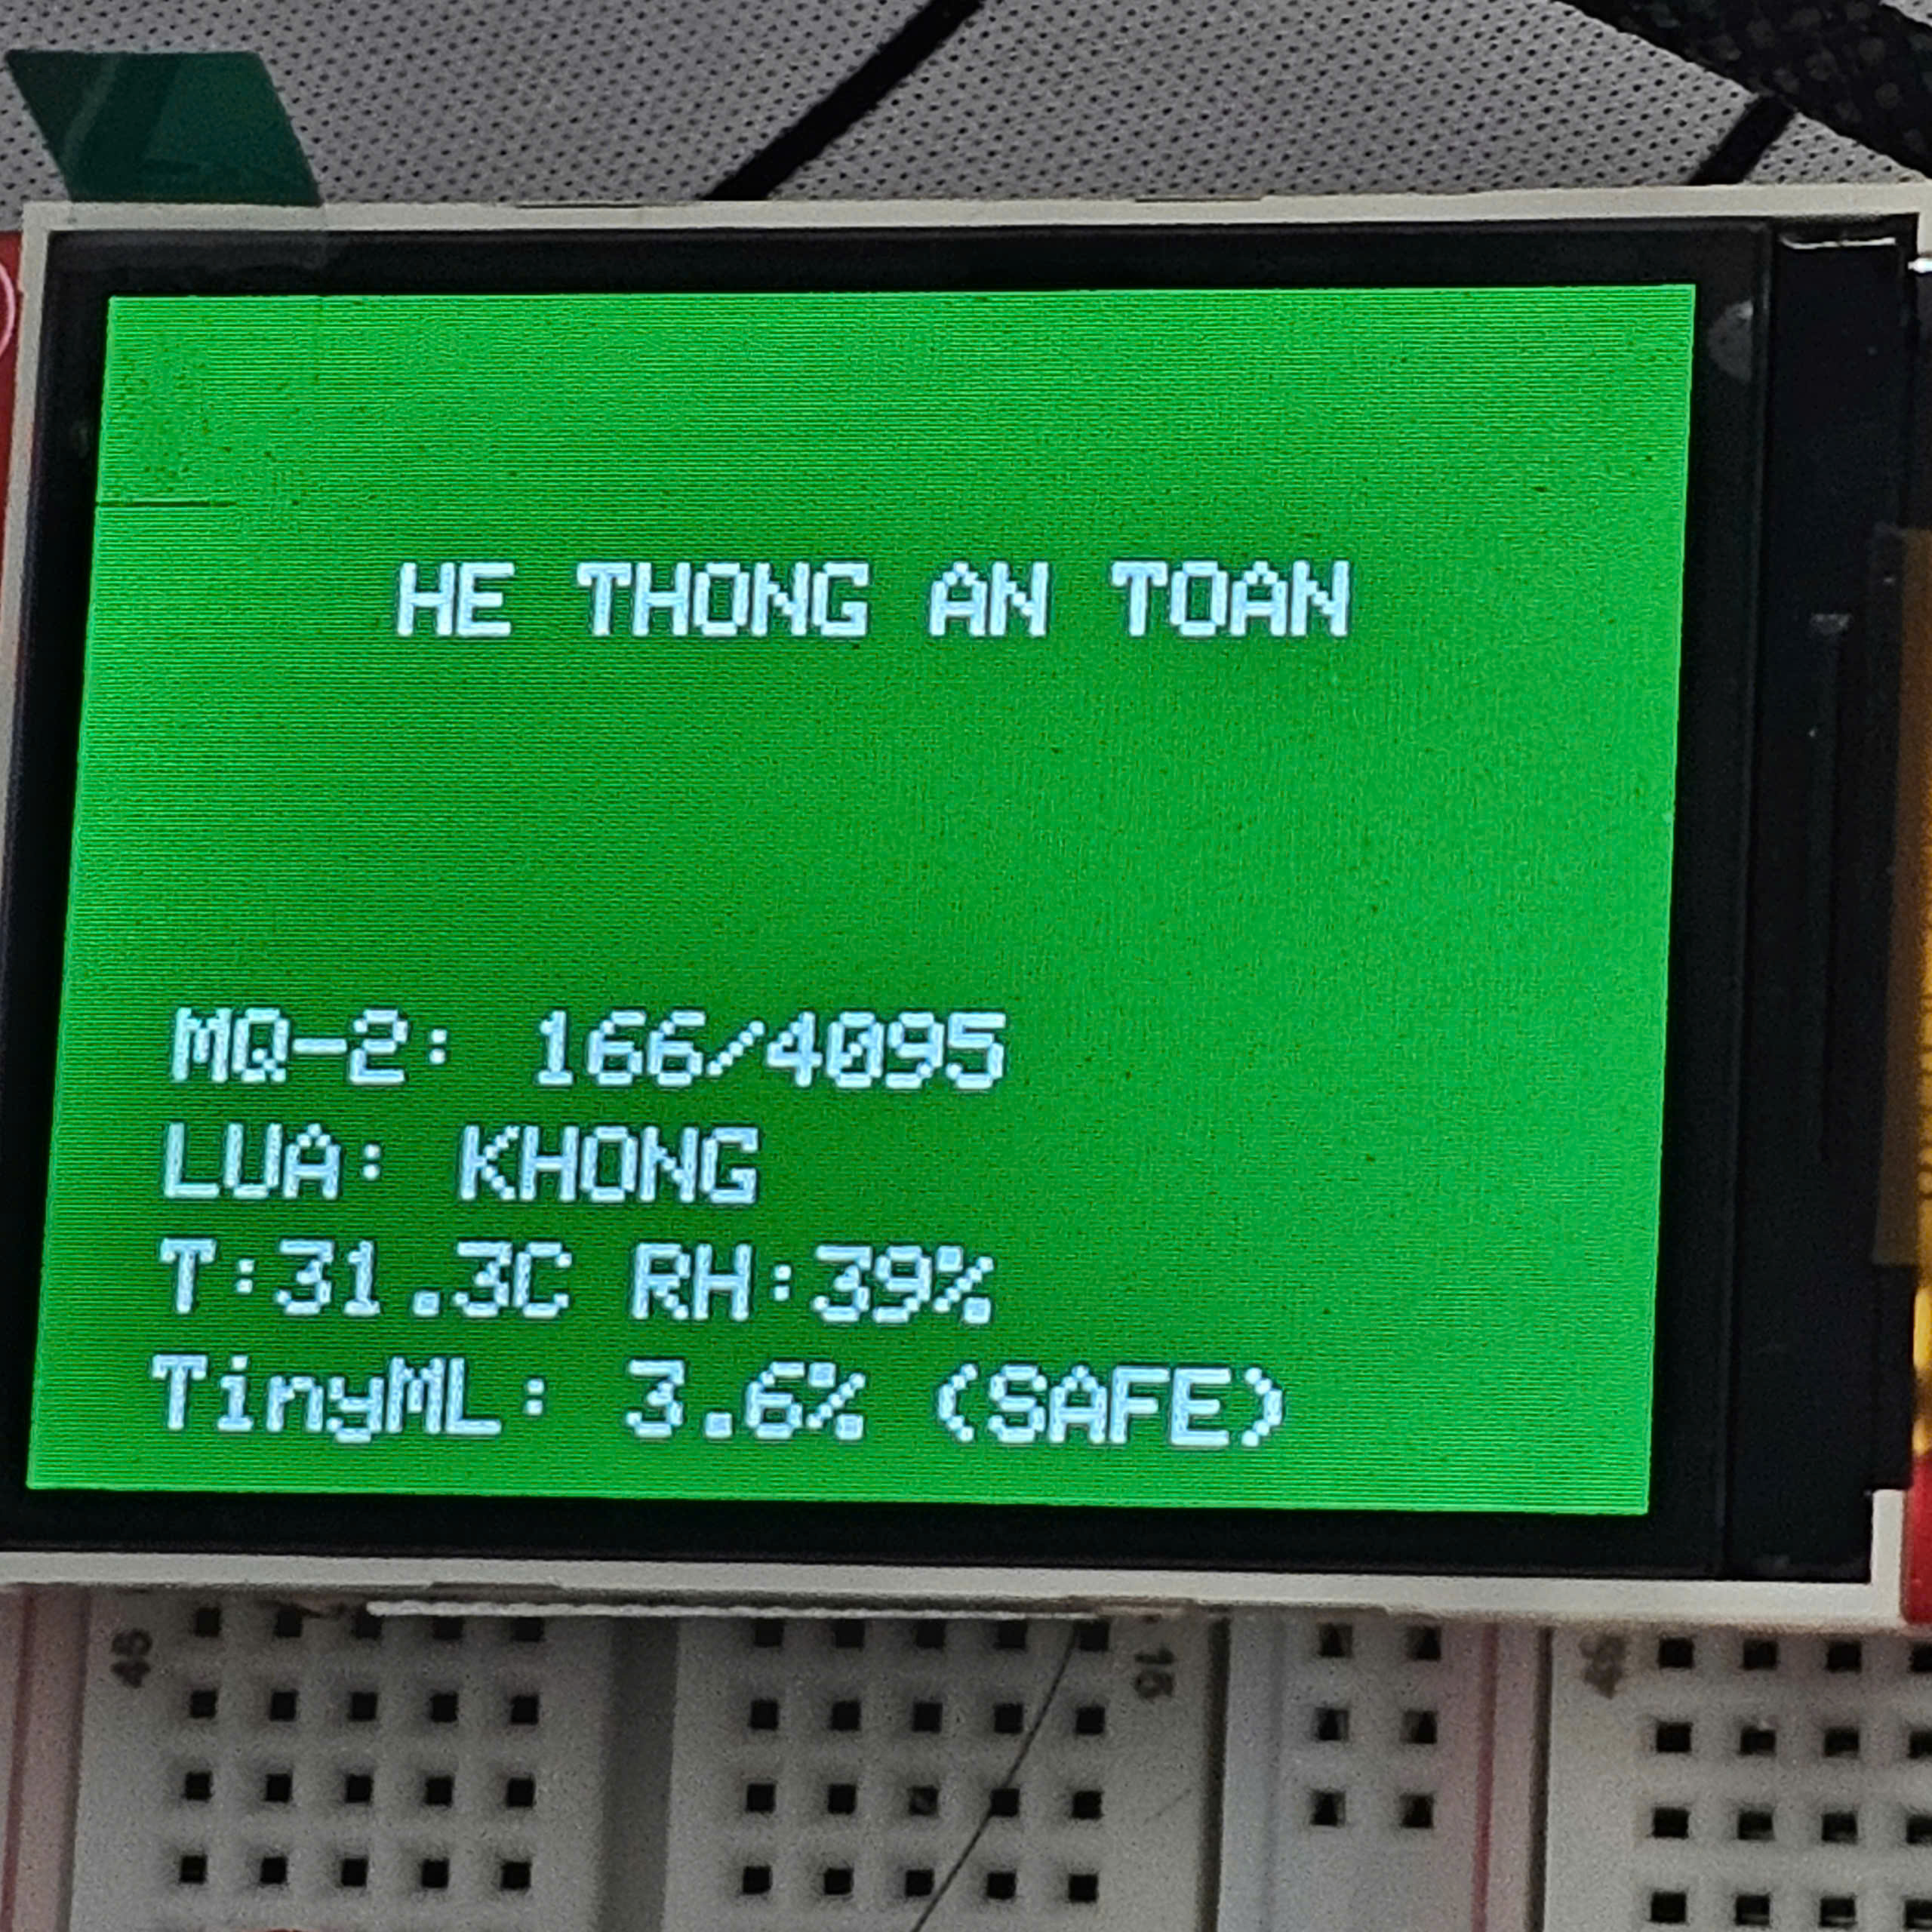
\includegraphics[width=\linewidth, height=6.0cm, keepaspectratio]{../../captured_picture/T04_1.jpg}
    \par\smallskip{\small (a) Trạng thái an toàn trên màn hình TFT (\texttt{T04\_1.jpg})}
  \end{minipage}
  \hfill
  \begin{minipage}[t]{0.48\textwidth}
    \centering
    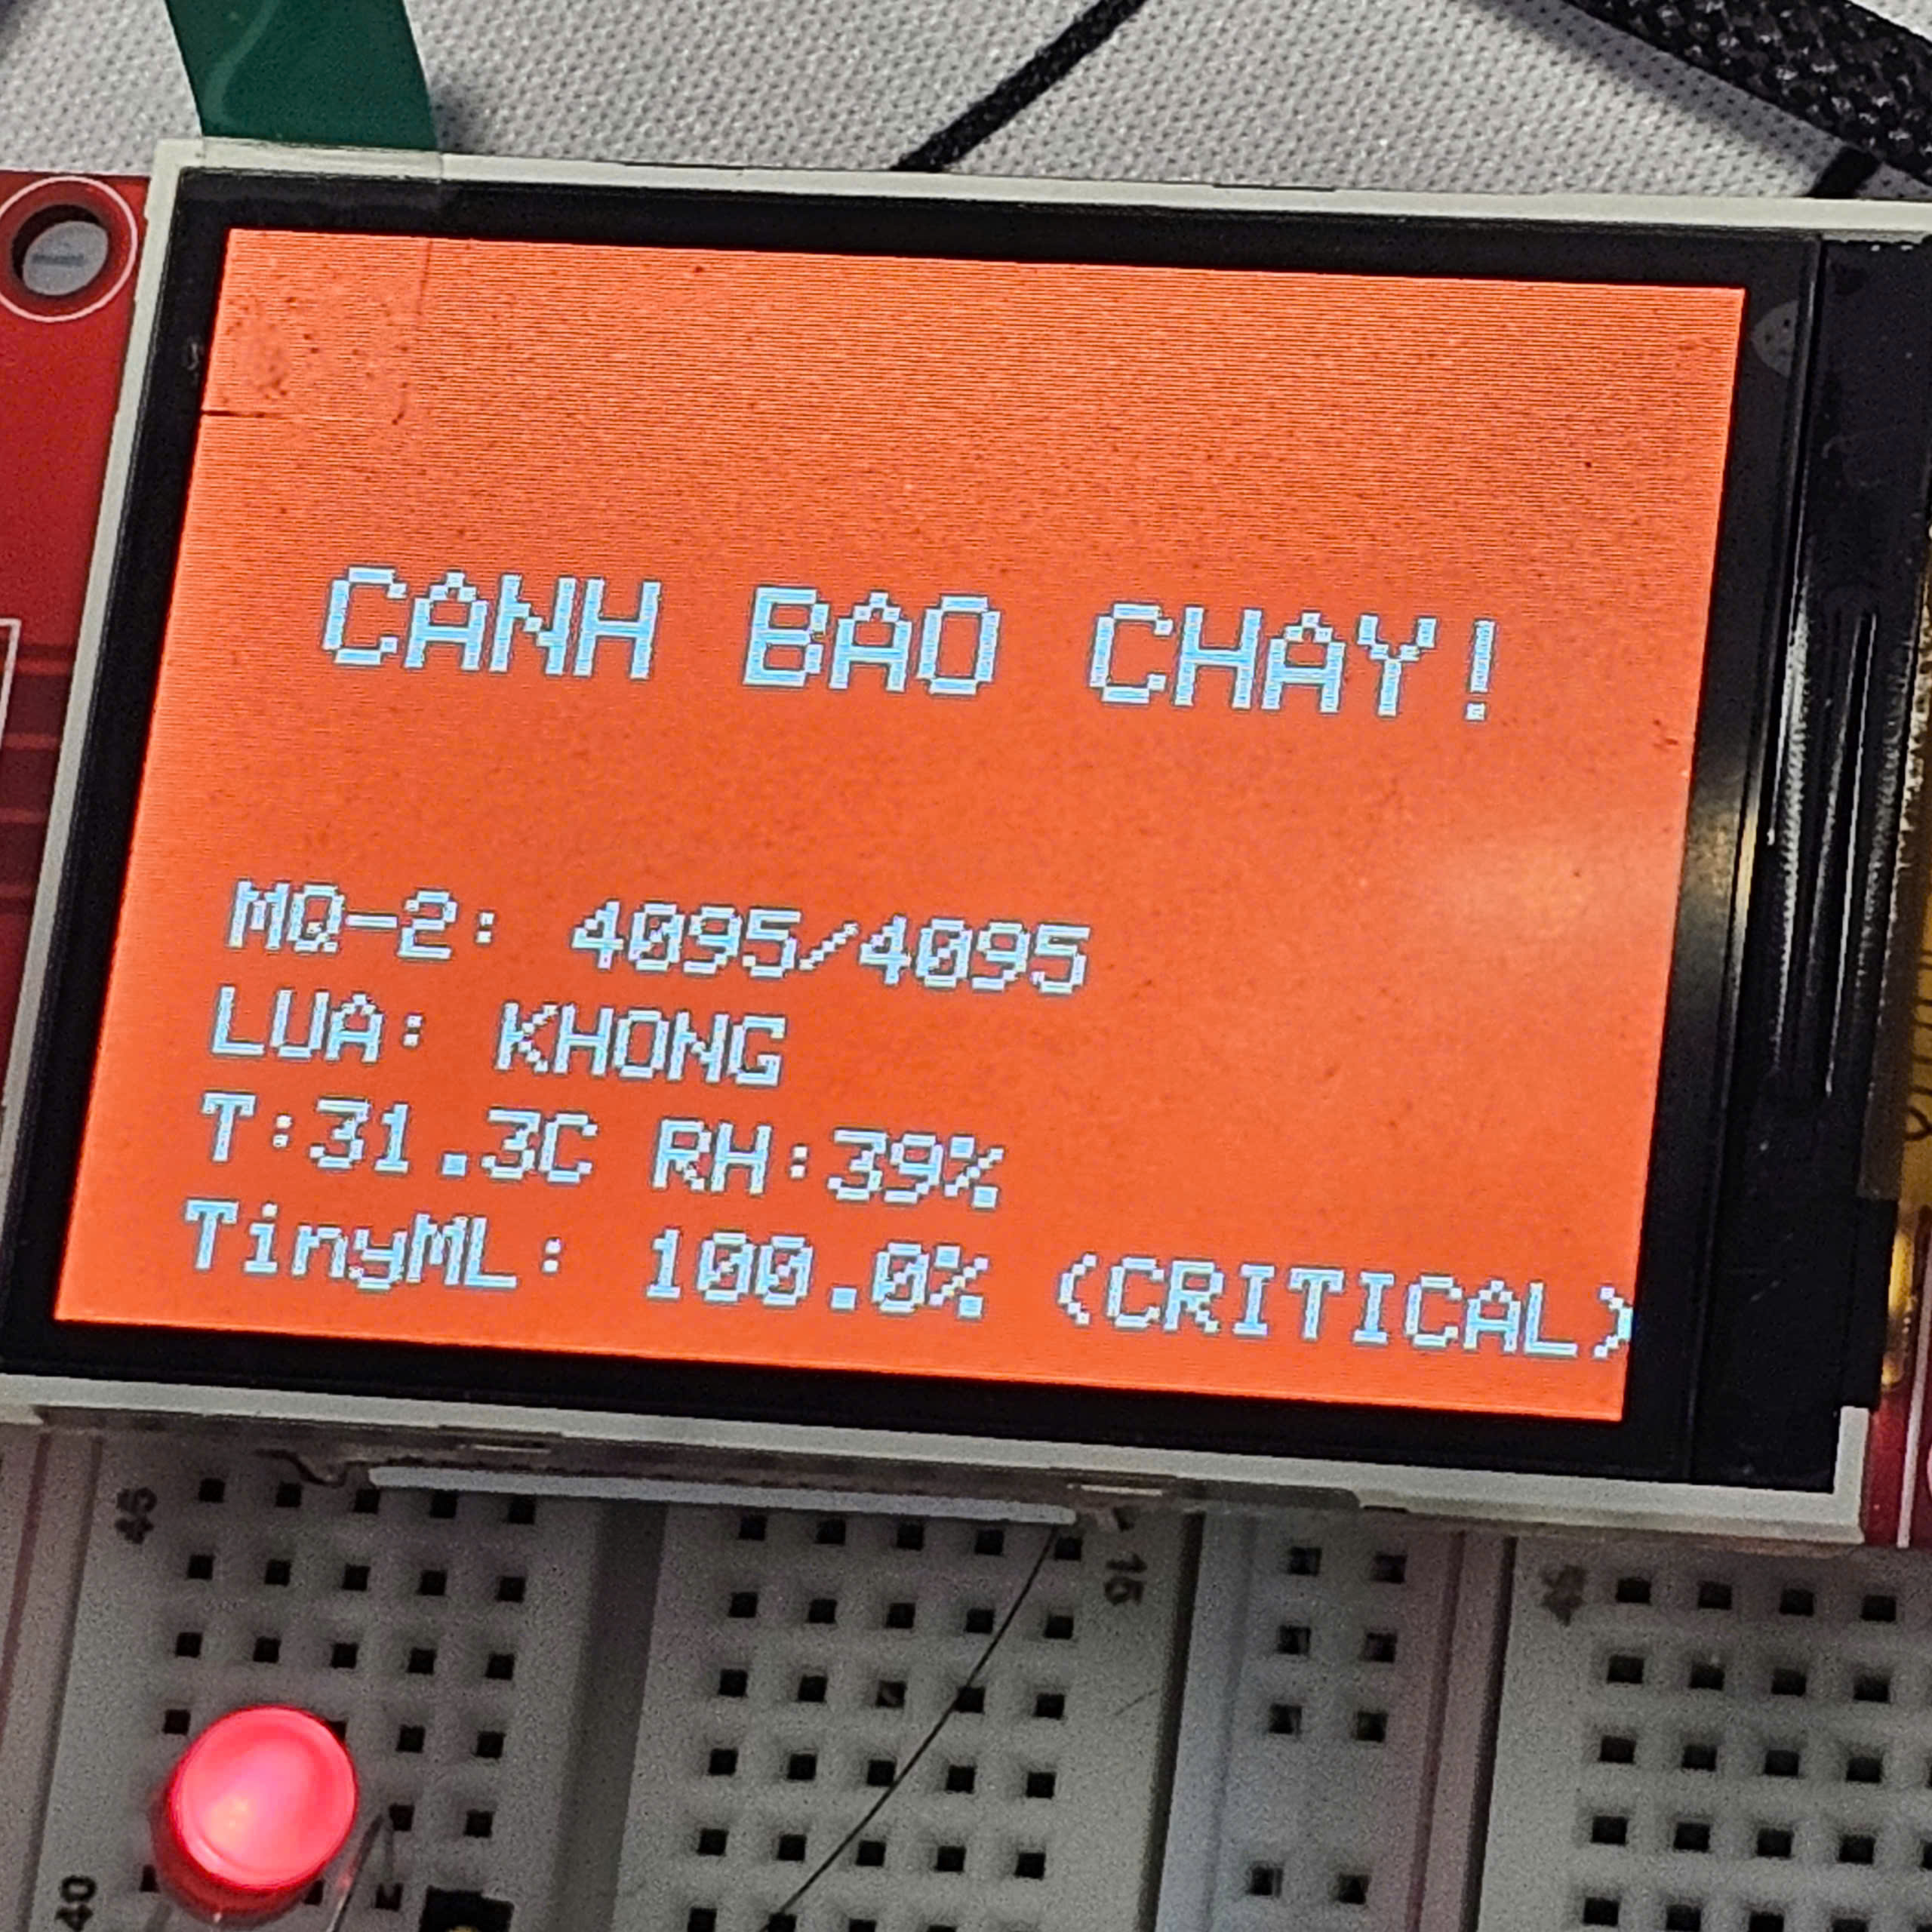
\includegraphics[width=\linewidth, height=6.0cm, keepaspectratio]{../../captured_picture/T04_2.jpg}
    \par\smallskip{\small (b) Trạng thái cảnh báo cháy trên màn hình TFT (\texttt{T04\_2.jpg})}
  \end{minipage}
  \caption{Hình ảnh phần cứng thực tế node YoloUNO ESP32-S3 và màn hình TFT ILI9341 ở hai trạng thái vận hành (T04)}
  \label{fig:so-do-dau-noi}
\end{figure}

\subsection{Firmware trên thiết bị}
\label{subsec:firmware-thiet-bi}

\subsubsection{Node cảm biến cháy và chấp hành YoloUNO (T04, T08)}
\label{subsubsec:node-1}

Firmware của End-Node được phát triển trên môi trường \textbf{PlatformIO} với cấu hình \texttt{[env:yolo\_uno]} trong tệp \texttt{01\_Firmware\_EndNode/platformio.ini}: nền tảng \texttt{espressif32}, bo mạch \texttt{esp32-s3-devkitc-1}, framework \texttt{arduino}, tốc độ Serial \texttt{115200} bps và cờ biên dịch \texttt{-D ARDUINO\_USB\_MODE=1}, \texttt{-D ARDUINO\_USB\_CDC\_ON\_BOOT=1}. Năm thư viện phụ thuộc gồm \texttt{Adafruit GFX Library}, \texttt{Adafruit ILI9341}, \texttt{ESP32Servo}, \texttt{DHT sensor library} và \texttt{Adafruit Unified Sensor}. Ngoài ra, thư mục \texttt{include/} có chuẩn bị sẵn tệp cấu hình \texttt{lv\_conf.h} (màu 16-bit, bộ nhớ đệm $32\text{ KB}$, bộ font Montserrat 12/14/32, giao diện tối) cho hướng mở rộng sang LVGL sau này; tuy nhiên ở phiên bản hiện thực chính thức, firmware điều khiển màn hình TFT ILI9341 trực tiếp bằng \texttt{Adafruit\_ILI9341} để tối ưu tốc độ vẽ lại màn hình và dung lượng Flash (vì vậy nhóm không khai báo tiêu chí \texttt{N03}).

Thay vì sử dụng hàm \texttt{delay()} gây nghẽn, vòng lặp \texttt{loop()} vận hành theo kiến trúc định thời không chặn (non-blocking cooperative scheduling) dựa trên \texttt{millis()} với ba chu kỳ độc lập và các cơ chế an toàn quan trọng:
\begin{enumerate}[leftmargin=*, itemsep=2pt]
  \item \textbf{Xử lý lệnh UART liên tục:} Hàm \texttt{processSerialCommands()} đọc bộ đệm 128 byte không chặn ở mỗi vòng lặp, nhận diện lệnh \texttt{alarm\_override}, \texttt{servo}, \texttt{buzzer}, \texttt{led} (tương thích cả định dạng JSON rút gọn lẫn định dạng RPC của ThingsBoard).
  \item \textbf{Cơ chế trễ (Hysteresis) và ưu tiên an toàn tuyệt đối:} Cảm biến MQ-2 kích hoạt khi $\text{ADC} \ge 1800$ và chỉ xóa khi $\text{ADC} \le 1650$; nhiệt độ DHT11 kích hoạt khi $T \ge 35.0^\circ\text{C}$ và xóa khi $T \le 34.0^\circ\text{C}$; cảm biến lửa kích hoạt tức thì khi \texttt{FLAME\_PIN == LOW}. Khi nhận lệnh điều khiển thủ công từ xa, cờ \texttt{manualOverrideUntil} giữ trạng thái thủ công trong $5000\text{ ms}$, nhưng nếu cảm biến phát hiện cháy thật (\texttt{!nextSafe}), firmware lập tức đặt \texttt{manualOverrideUntil = 0} để ép thực thi quy trình cứu hỏa.
  \item \textbf{Hiệu chỉnh tỷ số truyền cơ khí Servo:} Do liên kết cơ khí giữa trục Servo và cánh cửa mô hình có hành trình thực bằng một nửa góc quay trục, hằng số \texttt{SERVO\_COMMAND\_SCALE = 2} tự động nhân đôi góc logic ($0^\circ$--$90^\circ$) nhận từ Gateway sang góc vật lý ($0^\circ$--$180^\circ$, giới hạn tối đa \texttt{SERVO\_CLOSED\_ANGLE = 180}).
\end{enumerate}

Đoạn mã \ref{lst:main-loop} trích lược logic lấy mẫu, suy luận TinyML và xuất bản tin telemetry tại lõi hàm \texttt{loop()} trong \texttt{01\_Firmware\_EndNode/src/main.cpp}.

\begin{lstlisting}[language=C++, caption={Logic lấy mẫu đa cảm biến, suy luận TinyML và báo cáo UART trong \texttt{main.cpp}}, label={lst:main-loop}]
if (static_cast<uint32_t>(now - lastSensorSample) >= SENSOR_SAMPLE_INTERVAL_MS) {
  lastSensorSample = now;
  const int mq2Value = analogRead(MQ2_PIN);
  const bool flameDetected = digitalRead(FLAME_PIN) == LOW;
  if (!mq2AlarmActive && mq2Value >= MQ2_ALARM_THRESHOLD) mq2AlarmActive = true;
  else if (mq2AlarmActive && mq2Value <= MQ2_CLEAR_THRESHOLD) mq2AlarmActive = false;

  const bool nextSafe = !mq2AlarmActive && !flameDetected && !temperatureAlarmActive;
  const float curTemp = isnan(temperatureC) ? 28.0f : temperatureC;
  const float curHum  = isnan(humidityPercent) ? 65.0f : humidityPercent;
  const float aiRisk  = tinyml_predict_fire_risk(
      static_cast<float>(mq2Value), curTemp, flameDetected ? 1.0f : 0.0f, curHum);

  if (nextSafe != showingSafe) {
    if (!nextSafe) manualOverrideUntil = 0; // Real danger overrides manual state
    if (!nextSafe || now >= manualOverrideUntil) {
      showingSafe = nextSafe;
      showStatus(showingSafe, mq2Value, flameDetected, temperatureC, humidityPercent, aiRisk);
    }
  }
  if (static_cast<uint32_t>(now - lastSerialReport) >= SERIAL_REPORT_INTERVAL_MS) {
    lastSerialReport = now;
    Serial.printf("MQ-2 ADC: %d | Lua: %s | Nhiet do: %.1f C | Do am: %.0f%% | "
                  "AI Risk: %.1f%% | Trang thai: %s\n",
                  mq2Value, flameDetected ? "PHAT HIEN" : "KHONG",
                  temperatureC, humidityPercent, aiRisk * 100.0f,
                  showingSafe ? "AN TOAN" : "CANH BAO");
  }
}
\end{lstlisting}

\subsubsection{Webserver trên thiết bị (T07)}
\label{subsubsec:webserver-thiet-bi}

Trong phiên bản hiện thực này, nhóm \textbf{không triển khai Webserver trực tiếp trên ESP32-S3 (T07)}. Thay vào đó, giao diện giám sát và điều khiển cục bộ được đặt tập trung tại máy chủ HTTP nhúng của Local IoT Gateway (cổng \texttt{5050}, tiêu chí \texttt{T10} và \texttt{N06}, trình bày tại Mục \ref{subsec:iot-gateway}). Lựa chọn kiến trúc này giúp giải phóng toàn bộ ngăn xếp mạng TCP/IP trên vi điều khiển, đảm bảo tính định thời cứng cho vòng lặp đọc cảm biến $100\text{ ms}$, vẽ màn hình TFT SPI và suy luận TinyML mà không xảy ra gián đoạn do truy cập HTTP đồng thời.

\subsection{Truyền thông giữa các thiết bị}
\label{subsec:truyen-thong-thiet-bi}

Hệ thống sử dụng mô hình kết nối trực tiếp \textbf{UART USB-CDC 115200 bps} giữa End-Node YoloUNO (ESP32-S3) và Local IoT Gateway trên PC (không sử dụng BLE -- T03 hay ESP-NOW -- T06). Luồng truyền thông hai chiều được quản lý bởi lớp \path{HardwareSerialAdapter} và hàm \path{parse_uart_payload()} trong \path{02_Local_Gateway/hardware_gateway/LocalGateway.py}:
\begin{itemize}[leftmargin=*, itemsep=2pt]
  \item \textbf{Chiều Uplink (ESP32-S3 $\rightarrow$ PC):} \texttt{HardwareSerialAdapter} tự động quét các cổng COM dựa trên mô tả phần cứng (\texttt{ESP32}, \texttt{CH340}, \texttt{CP210}, \texttt{UART}, \texttt{USB SERIAL}, \texttt{303A}), mở cổng với \texttt{timeout=1.0 s} và xóa bộ đệm đầu vào. Hàm \texttt{parse\_uart\_payload()} hỗ trợ phân tích đồng thời cả chuỗi JSON chuẩn lẫn định dạng văn bản từ \texttt{main.cpp} bằng biểu thức chính quy, trích xuất đầy đủ các trường \texttt{smoke}, \texttt{flame}, \texttt{temperature}, \texttt{humidity}, \texttt{tinyml\_risk} và \texttt{status}.
  \item \textbf{Chiều Downlink (PC $\rightarrow$ ESP32-S3):} Lệnh điều khiển từ Cloud RPC hoặc Web Monitor được đưa vào \texttt{queue.Queue} và tuần tự hóa thành JSON kết thúc bằng \texttt{\textbackslash n} qua \texttt{write\_command()} có khóa đồng bộ \texttt{threading.Lock}, đảm bảo không xảy ra xung đột luồng trên cổng nối tiếp.
\end{itemize}

Hình \ref{fig:uart-gateway-log} minh chứng nhật ký truyền nhận hai chiều thực tế giữa bo mạch ESP32-S3 và Local Gateway trên Terminal (tiêu chí \texttt{T08}).

\begin{figure}[H]
  \centering
  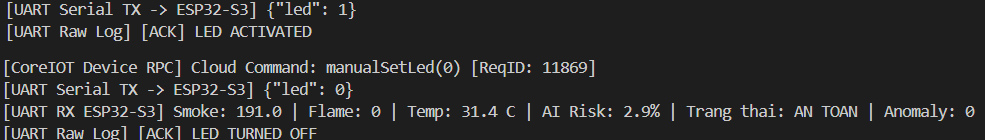
\includegraphics[width=0.92\textwidth]{../../captured_picture/T08.png}
  \caption{Minh chứng luồng truyền nhận UART hai chiều giữa ESP32-S3 và Local Gateway trên PC (T08 -- \texttt{T08.png})}
  \label{fig:uart-gateway-log}
\end{figure}

\subsection{IoT Gateway}
\label{subsec:iot-gateway}

Phân hệ Local IoT Gateway được xây dựng bằng Python 3 trong thư mục \path{02_Local_Gateway/} với các thư viện chính gồm \texttt{pyserial}, \texttt{paho-mqtt}, \texttt{scikit-learn}, \texttt{numpy} và các mô-đun chuẩn (\texttt{sqlite3}, \path{http.server}, \texttt{socketserver}, \texttt{threading}, \texttt{queue}). Hệ thống cung cấp các trình khởi chạy tự động gồm \path{run_system.py} (tại thư mục gốc), \path{02_Local_Gateway/run_hardware_gateway.py} và \path{02_Local_Gateway/start_system.py}, cho phép tự dò cổng COM, tự phát hiện container ThingsBoard cục bộ (cổng \texttt{1883}/\texttt{9090}), mở đồng thời hai bảng điều khiển trên trình duyệt và xử lý tín hiệu \texttt{SIGINT}/\texttt{SIGTERM} để giải phóng cổng COM an toàn khi nhấn \texttt{Ctrl+C}.

\textbf{Cơ chế lưu đệm ngoại tuyến SQLite WAL và đồng bộ Gateway (T08, T15):}
Lớp \path{OfflineBufferRepository} trong \path{02_Local_Gateway/ui/gateway_infrastructure.py} khởi tạo cơ sở dữ liệu \path{gateway_hardware_buffer.db} ở chế độ Write-Ahead Logging với lược đồ bảng:
\begin{center}
  \texttt{telemetry\_buffer(id INTEGER PRIMARY KEY AUTOINCREMENT, payload TEXT, timestamp REAL, synced INTEGER DEFAULT 0)}
\end{center}
Mỗi khi nhận bản tin mới từ UART, luồng chính tính toán kết quả Isolation Forest (\texttt{is\_anomaly}, \texttt{anomaly\_score}), sinh chuỗi \texttt{alarm\_status} và \texttt{alarm\_notification}, chèn ngay bản tin vào SQLite (\texttt{synced = 0}), rồi đẩy tức thời qua MQTT QoS 1 nếu kết nối đang khả dụng. Song song đó, luồng nền \texttt{sync\_worker} thức dậy mỗi $3.0\text{ s}$: khi cờ \texttt{cloud\_connected} chuyển sang \texttt{True}, tiến trình truy vấn tối đa 25 bản ghi chưa đồng bộ theo thứ tự FIFO, phát hành lên chủ đề \texttt{v1/devices/me/telemetry} (hoặc \texttt{v1/gateway/telemetry} cho thiết bị con \texttt{YOLOUNO\_FIRE\_NODE\_01} khi bật cờ \texttt{--gateway-api}), đánh dấu \texttt{synced = 1} khi nhận mã \texttt{MQTT\_ERR\_SUCCESS}, và dọn các bản ghi đã đồng bộ cũ hơn 7 ngày (\texttt{purge\_synced}).

\begin{lstlisting}[language=Python, caption={Luồng đồng bộ bù FIFO từ SQLite WAL lên CoreIOT/ThingsBoard trong \texttt{LocalGateway.py}}, label={lst:sync-worker}]
def sync_worker(self):
    while self.running:
        with self.telemetry_lock:
            cloud_ok = self.latest_telemetry["cloud_connected"]
            self.latest_telemetry["buffer_count"] = self.buffer_repo.count_unsynced()
        if cloud_ok:
            unsynced = self.buffer_repo.fetch_unsynced(limit=25)
            synced_ids = []
            for rec_id, payload_str in unsynced:
                if self.use_gateway_api:
                    rec_data = json.loads(payload_str)
                    gw_dev = "YOLOUNO_FIRE_NODE_01" if self.device_name == "FireAlarm_Gateway" else self.device_name
                    gw_msg = {gw_dev: [{"ts": int(time.time() * 1000), "values": rec_data}]}
                    info = self.mqtt_client.publish(GATEWAY_TELEMETRY_TOPIC, json.dumps(gw_msg), qos=1)
                else:
                    info = self.mqtt_client.publish(TELEMETRY_TOPIC, payload_str, qos=1)
                if info.rc == mqtt.MQTT_ERR_SUCCESS:
                    synced_ids.append(rec_id)
                else:
                    break
            if synced_ids:
                self.buffer_repo.mark_synced(synced_ids)
            self.buffer_repo.purge_synced(older_than_days=7.0)
        time.sleep(3.0)
\end{lstlisting}

\textbf{Giao diện giám sát -- điều khiển cục bộ SCADA (T10):}
Lớp \texttt{EmbeddedWebMonitor} phục vụ giao diện web chuẩn Keen Dashboards tại \texttt{http://localhost:5050}. Giao diện bao gồm thanh trạng thái trên cùng (chế độ Gateway, trạng thái kết nối CoreIOT Online/Offline Buffering, trạng thái End Node dựa trên chu kỳ kiểm tra $6\text{ s}$ và số bản ghi đang đệm trong SQLite), biểu ngữ cảnh báo cháy đỏ toàn chiều rộng, 5 thẻ thông số thời gian thực (Smoke Concentration ADC, Ambient Temperature, Flame Optical Sensor, Emergency Fire Door Servo, AI Isolation Forest), khu vực điều khiển cưỡng bức từng cơ cấu chấp hành kèm hai nút khẩn cấp (\texttt{TRIGGER EMERGENCY LOCKDOWN} và \texttt{RESTORE NORMAL OPERATION}). Hình \ref{fig:local-scada} trình bày giao diện hoạt động thực tế của Local SCADA Web Monitor.

\begin{figure}[H]
  \centering
  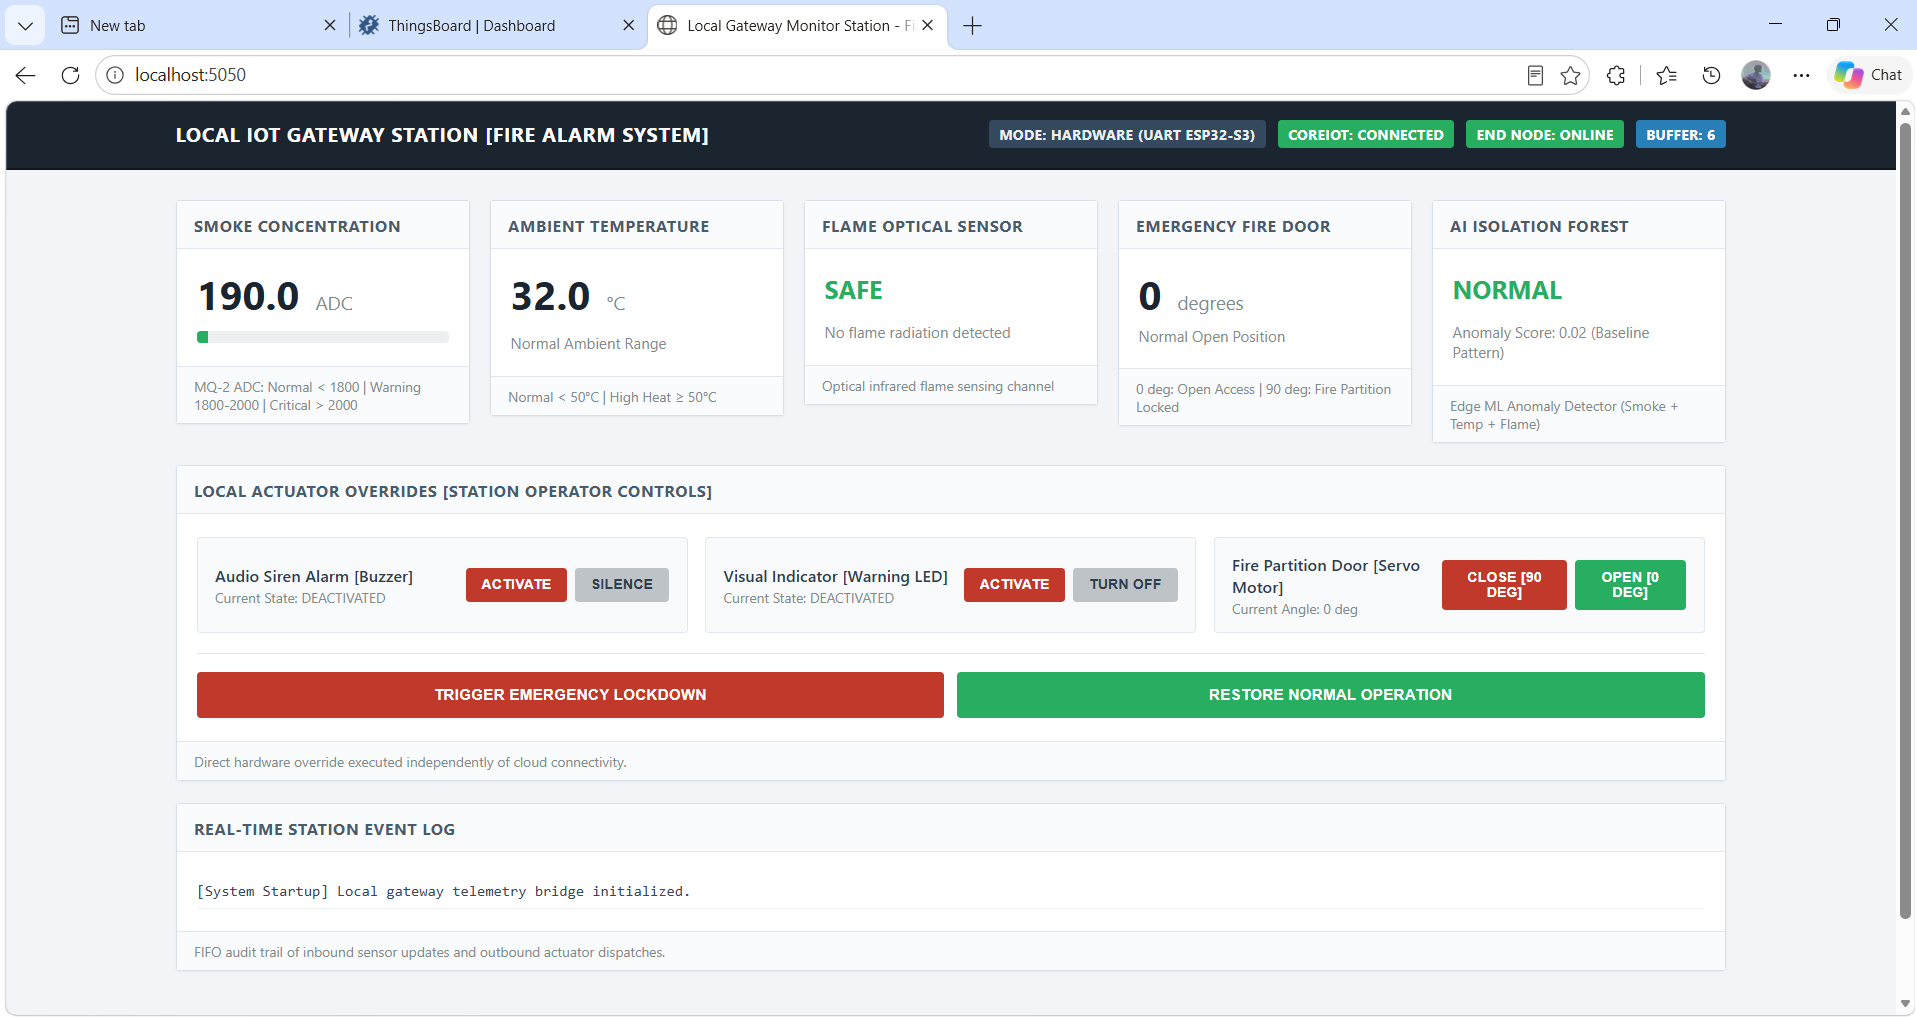
\includegraphics[width=0.95\textwidth]{../../captured_picture/T10.png}
  \caption{Giao diện giám sát và điều khiển SCADA cục bộ trên Local Gateway tại cổng 5050 (T10 -- \texttt{T10.png})}
  \label{fig:local-scada}
\end{figure}

\subsection{Trí tuệ nhân tạo}
\label{subsec:tri-tue-nhan-tao}

\subsubsection{Thu thập và chuẩn bị dữ liệu}
\label{subsubsec:ai-du-lieu}

Đối với mô hình TinyML trên vi điều khiển (tiêu chí \texttt{T05}), kịch bản \path{01_Firmware_EndNode/tinyml/train_tinyml.py} thực hiện tổng hợp tập dữ liệu đa chiều gồm \textbf{2.500 mẫu} (hàm \path{generate_synthetic_dataset()} với \texttt{num\_samples=2500}, \texttt{random\_state=42}) phản ánh đặc tính vật lý của ba cảm biến thực tế trên bo mạch, với 4 đặc trưng đầu vào (\path{MQ2_ADC}, \texttt{TEMPERATURE}, \texttt{HUMIDITY}, \texttt{FLAME}) và 2 lớp nhãn (0: \textit{Safe}, 1: \textit{Fire Hazard}):
\begin{itemize}[leftmargin=*, itemsep=2pt]
  \item \textbf{Lớp an toàn (Safe -- $65\%$, 1.625 mẫu):} $\text{MQ-2} \sim \mathcal{N}(180, 40^2)$ giới hạn $[80, 500]$, nhiệt độ $\sim \mathcal{N}(28.0, 3.0^2)$ trong $[20.0, 38.0]^\circ\text{C}$, độ ẩm $\sim \mathcal{N}(65.0, 8.0^2)$ trong $[40.0, 90.0]\%$, $\text{Flame} = 0$.
  \item \textbf{Lớp nguy cơ cháy (Fire Hazard -- $35\%$, 875 mẫu):} Phân bổ theo ba kịch bản cháy thực tế: (A) \textit{Cháy bùng có lửa} ($40\%$: $\text{MQ-2} \in [500, 2500]$, $T \in [32, 60]^\circ\text{C}$, $\text{RH} \in [20, 55]\%$, $\text{Flame}=1$); (B) \textit{Cháy sinh khói/gas đậm đặc} ($40\%$: $\text{MQ-2} \in [1800, 3800]$, $T \in [28, 50]^\circ\text{C}$, $\text{Flame} \in \{0,1\}$ với xác suất $0.7/0.3$); (C) \textit{Quá nhiệt cháy âm ỉ} ($20\%$: $\text{MQ-2} \in [900, 2200]$, $T \in [50, 68]^\circ\text{C}$, $\text{RH} \in [20, 45]\%$, $\text{Flame} \in \{0,1\}$ với xác suất $0.8/0.2$).
\end{itemize}

Tập dữ liệu được xáo trộn và tách theo tỉ lệ $80/20$ phân tầng (\texttt{stratify=y}): \textbf{2.000 mẫu huấn luyện} và \textbf{500 mẫu kiểm thử}. Các đặc trưng được chuẩn hóa Z-score sử dụng giá trị trung bình và độ lệch chuẩn tính hoàn toàn trên tập huấn luyện nhằm tránh rò rỉ dữ liệu.

Đối với mô hình Isolation Forest trên Local Gateway (tiêu chí \texttt{T09}), lớp \texttt{IsolationDetector} (\texttt{02\_Local\_Gateway/ui/isolation\_detector.py}) khởi tạo tập nền an toàn gồm 100 mẫu phủ toàn bộ dải vận hành dưới ngưỡng báo động ($\text{smoke} < 1800\text{ ADC}$, $T \in [15, 34]^\circ\text{C}$, $\text{flame}=0$) để tránh phụ thuộc vào độ lệch nền (offset) của từng cảm biến MQ-2, đồng thời duy trì hàng đợi cửa sổ trượt \texttt{deque(maxlen=200)} trong quá trình vận hành.

\subsubsection{Huấn luyện và đánh giá mô hình}
\label{subsubsec:ai-huan-luyen}

\textbf{Mô hình TinyML (T05):} Sử dụng \texttt{LogisticRegression(C=1.0, max\_iter=1000, random\_state=42)} từ \texttt{scikit-learn}. Trên tập kiểm thử 500 mẫu, mô hình đạt độ chính xác tổng thể \textbf{100.00\%} như thể hiện trong kết quả đầu ra của \texttt{train\_tinyml.py} (Hình \ref{fig:tinyml-train}) và bảng tham số trích xuất trực tiếp từ \texttt{tinyml\_fire\_model.h} tại Bảng \ref{tab:tham-so-tinyml}. Dấu của các trọng số hoàn toàn phù hợp quy luật vật lý: trọng số dương lớn cho khói MQ-2 ($+3.760794$), nhiệt độ ($+1.929540$) và lửa ($+1.876357$), trong khi trọng số âm cho độ ẩm ($-1.685517$) vì môi trường cháy thường khô nóng.

\begin{table}[H]
  \centering
  \caption{Tham số chuẩn hóa Z-score và trọng số mô hình TinyML trích xuất từ \texttt{tinyml\_fire\_model.h}}
  \label{tab:tham-so-tinyml}
  \renewcommand{\arraystretch}{1.25}
  \begin{tabularx}{\textwidth}{|L{0.26\textwidth}|C{0.22\textwidth}|C{0.22\textwidth}|C{0.22\textwidth}|}
    \hline
    \rowcolor{iotTableHead}
    \textbf{Đặc trưng đầu vào} & \textbf{Trung bình ($\mu_i$)} & \textbf{Độ lệch chuẩn ($\sigma_i$)} & \textbf{Trọng số ($w_i$)} \\
    \hline
    \texttt{MQ2\_ADC} (0--4095) & 826.217565 & 1007.851218 & $+3.760794$ \\
    \hline
    \texttt{TEMPERATURE} ($^\circ\text{C}$) & 34.104391 & 10.501738 & $+1.929540$ \\
    \hline
    \texttt{HUMIDITY} ($\%$) & 55.451318 & 15.155835 & $-1.685517$ \\
    \hline
    \texttt{FLAME} (0 hoặc 1) & 0.194500 & 0.395815 & $+1.876357$ \\
    \hline
    \multicolumn{3}{|l|}{\textbf{Hệ số tự do (\texttt{TINYML\_BIAS}):}} & $-1.230645$ \\
    \hline
  \end{tabularx}
\end{table}

\begin{figure}[H]
  \centering
  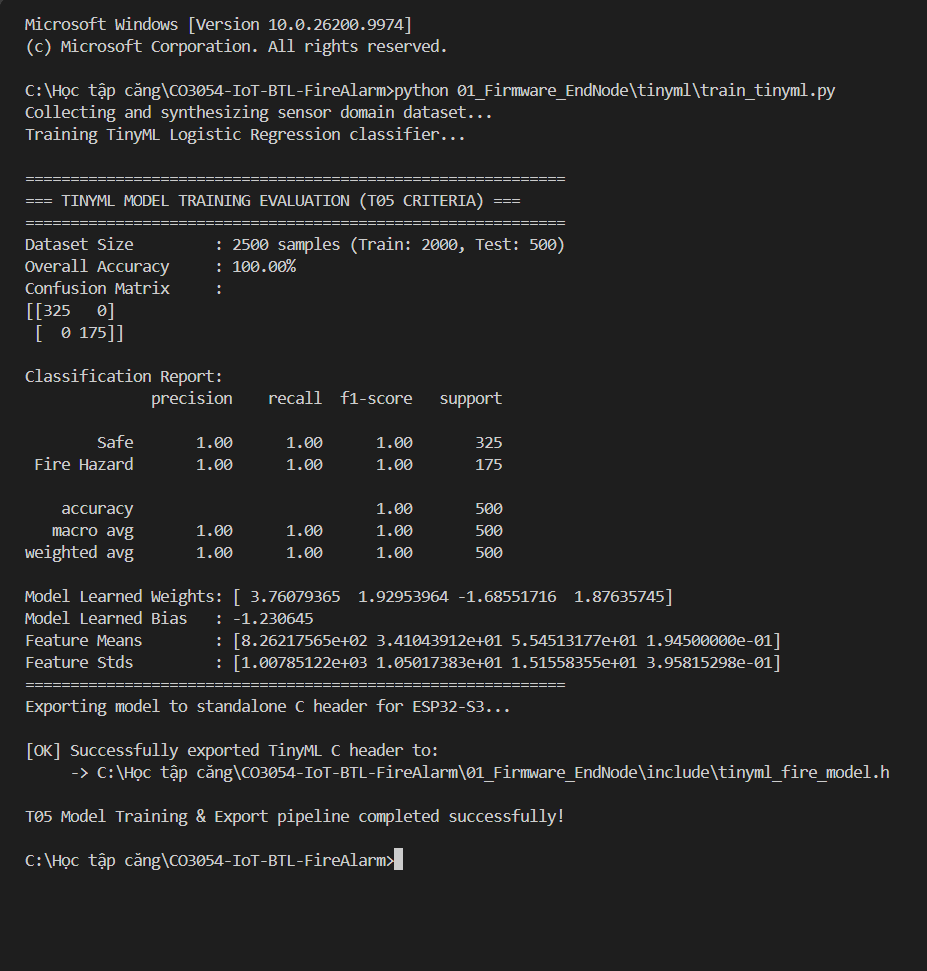
\includegraphics[width=0.9\textwidth]{../../captured_picture/T05.png}
  \caption[Kết quả huấn luyện TinyML và xuất tệp \texttt{tinyml\_fire\_model.h} (T05)]{Kết quả huấn luyện, đánh giá ma trận nhầm lẫn và xuất tệp \texttt{tinyml\_fire\_model.h} từ \texttt{train\_tinyml.py} (T05 -- \texttt{T05.png})}
  \label{fig:tinyml-train}
\end{figure}

\textbf{Mô hình Isolation Forest trên Local Gateway (T09):} Sử dụng thuật toán \texttt{IsolationForest} với siêu tham số \path{n_estimators=100}, \path{contamination=0.05} và \path{random_state=42}. Khi nhận mẫu đầu vào $[s, t, f]$, hệ thống kiểm tra tính hữu hạn (\path{math.isfinite}) để tránh lỗi \texttt{NaN}/\texttt{Inf} khi cảm biến đang làm nóng, đánh giá điều kiện bất thường cứng khớp ngưỡng firmware ($f > 0.5$ hoặc $s \ge 1800$ hoặc $t \ge 35.0^\circ\text{C}$), tính điểm \path{anomaly_score} theo phương trình \eqref{eq:iforest-score} và gán cờ \path{is_anomaly = 1} khi bộ dự đoán trả về $-1$, \path{anomaly_score >= 0.65} hoặc thỏa điều kiện cứng (khi đó điểm được nâng tối thiểu lên $0.90$). Hình \ref{fig:isolation-forest} minh chứng kết quả phát hiện thời gian thực trên Local Gateway ở hai trạng thái \texttt{NORMAL} và \texttt{ANOMALY DETECTED}.

\begin{figure}[H]
  \centering
  \begin{minipage}[t]{0.48\textwidth}
    \centering
    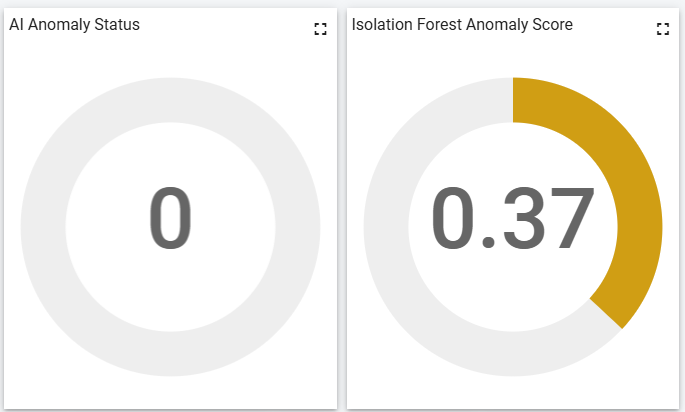
\includegraphics[width=\linewidth, height=4.8cm, keepaspectratio]{../../captured_picture/T09_1.png}
    \par\smallskip{\small (a) Trạng thái bình thường (\texttt{T09\_1.png})}
  \end{minipage}
  \hfill
  \begin{minipage}[t]{0.48\textwidth}
    \centering
    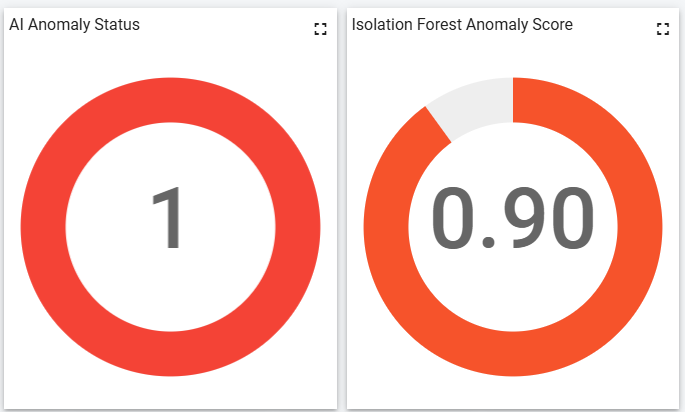
\includegraphics[width=\linewidth, height=4.8cm, keepaspectratio]{../../captured_picture/T09_2.png}
    \par\smallskip{\small (b) Phát hiện bất thường cháy (\texttt{T09\_2.png})}
  \end{minipage}
  \caption{Kết quả suy luận phát hiện bất thường đa biến bằng Isolation Forest trên Local Gateway (T09)}
  \label{fig:isolation-forest}
\end{figure}

\subsubsection{Triển khai mô hình}
\label{subsubsec:ai-trien-khai}

Hàm \path{export_c_header()} trong \path{train_tinyml.py} sinh trực tiếp tệp \path{01_Firmware_EndNode/include/tinyml_fire_model.h} gồm các hằng số mảng \texttt{static const float} và ba hàm nội tuyến \texttt{static inline}: \path{tinyml_sigmoid(float z)} (có chặn bão hòa tại $z > 12.0$ và $z < -12.0$ tránh tràn số), \path{tinyml_predict_fire_risk()} và \path{tinyml_get_risk_label()} phân chia ngưỡng rủi ro: $\ge 0.70 \rightarrow \texttt{CRITICAL}$, $\ge 0.40 \rightarrow \texttt{WARNING}$, $< 0.40 \rightarrow \texttt{SAFE}$.

Mô hình có dung lượng bộ nhớ ước tính chỉ khoảng \textbf{128 byte RAM}, hoàn toàn không sử dụng bộ nhớ động (zero heap allocation), được nhúng qua chỉ thị \texttt{\#include "tinyml\_fire\_model.h"} trong \texttt{main.cpp}. Kết quả xác suất cháy được hiển thị đồng thời trên dòng thứ 4 màn hình TFT ILI9341 (Hình \ref{fig:so-do-dau-noi}) và truyền lên Gateway qua trường \texttt{AI Risk} trong chuỗi Serial (Hình \ref{fig:tinyml-serial}).

\begin{figure}[H]
  \centering
  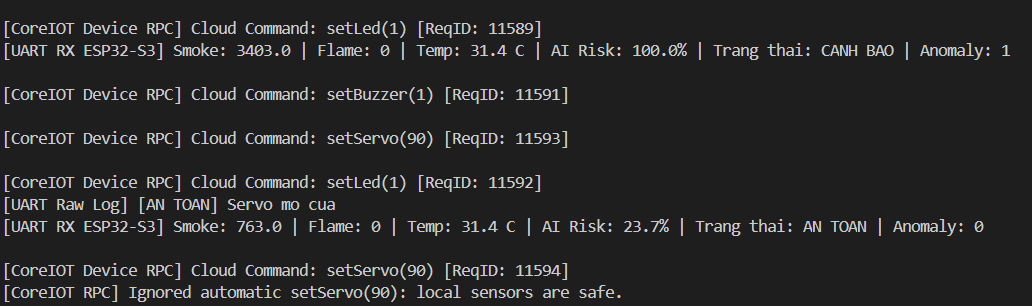
\includegraphics[width=0.92\textwidth]{../../captured_picture/T04_3.png}
  \caption{Minh chứng nhật ký Serial hiển thị xác suất rủi ro cháy \texttt{AI Risk} suy luận trực tiếp bởi TinyML trên ESP32-S3 (T04 -- \texttt{T04\_3.png})}
  \label{fig:tinyml-serial}
\end{figure}

\subsection{Nền tảng CoreIOT}
\label{subsec:nen-tang-coreiot}

\subsubsection{Device profile, template và dashboard (T11)}
\label{subsubsec:coreiot-dashboard}

Thay vì cấu hình thủ công trên giao diện web, nhóm xây dựng công cụ cấp phát tự động \path{02_Local_Gateway/dashboard/setup_thingsboard_dashboard.py}. Script thực hiện tuần tự 4 bước qua REST API của ThingsBoard: (1) chờ Spring Boot khởi động hoàn tất (timeout $180\text{ s}$); (2) đăng nhập tài khoản Tenant (\path{tenant@thingsboard.org}) để nhận mã JWT; (3) tạo hoặc truy xuất thiết bị \path{FireAlarm_Gateway} với \texttt{type = "Gateway"}, cờ \path{additionalInfo.gateway = true} và gán mã xác thực \path{i2tchqq1390qcxhun4zr}; (4) truy vấn các template widget hệ thống chuẩn của ThingsBoard 3.x, lắp ghép thành bảng điều khiển \textit{Industrial Fire Alarm \& Suppression System} gồm \textbf{10 widget} trên lưới 24 cột (cửa sổ thời gian thực 5 phút, chu kỳ $1\text{ s}$) và xuất lược đồ ra tệp \path{thingsboard_dashboard.json}. Danh sách chi tiết 10 widget được tổng hợp ở Bảng \ref{tab:tb-widgets} và ảnh chụp thực tế tại Hình \ref{fig:tb-dashboard}.

\begin{table}[htbp]
  \centering
  \caption[Cấu hình 10 widget trên ThingsBoard Industrial Dashboard]{Cấu hình 10 widget trên ThingsBoard Industrial Dashboard (\texttt{thingsboard\_dashboard.json})}
  \label{tab:tb-widgets}
  \renewcommand{\arraystretch}{1.22}
  \begin{tabularx}{\textwidth}{|C{0.05\textwidth}|L{0.25\textwidth}|L{0.23\textwidth}|C{0.14\textwidth}|Y|}
    \hline
    \rowcolor{iotTableHead}
    \textbf{STT} & \textbf{Tên Widget} & \textbf{Loại Widget (FQN)} & \textbf{Vị trí (r,c,w$\times$h)} & \textbf{Khóa dữ liệu / RPC} \\
    \hline
    1 & MQ-2 Raw ADC & Radial Gauge & (0,0, 5$\times$6) & \texttt{smoke} ($0$--$4095$; xanh $<1800$, cam $1800$--$2000$, đỏ $>2000$) \\
    \hline
    2 & Flame Detector Status & Digital Simple Gauge & (0,5, 5$\times$6) & \texttt{flame} ($0$: xanh, $1$: đỏ) \\
    \hline
    3 & Ambient Temperature & Value Card & (0,10, 4$\times$6) & \texttt{temperature} ($^\circ\text{C}$, icon nhiệt kế) \\
    \hline
    4 & AI Anomaly Status & Digital Simple Gauge & (0,14, 5$\times$6) & \texttt{is\_anomaly} ($0$ hoặc $1$) \\
    \hline
    5 & Isolation Forest Anomaly Score & Digital Simple Gauge & (0,19, 5$\times$6) & \texttt{anomaly\_score} ($0.00$--$1.00$) \\
    \hline
    6 & Environmental Telemetry History & Timeseries Chart & (6,0, 15$\times$7) & 4 kênh: \texttt{smoke}, \texttt{temperature}, \texttt{flame}, \texttt{anomaly\_score} \\
    \hline
    7 & Master Alarm Override & Round Switch (RPC) & (6,15, 3$\times$7) & \texttt{getAlarmOverride} / \texttt{setAlarmOverride} \\
    \hline
    8 & Alarm Siren Buzzer & Switch Control (RPC) & (6,18, 3$\times$7) & \texttt{getBuzzer} / \texttt{manualSetBuzzer} \\
    \hline
    9 & Strobe LED Beacon & Switch Control (RPC) & (6,21, 3$\times$7) & \texttt{getLed} / \texttt{manualSetLed} \\
    \hline
    10 & T13: Emergency Alarm Notification & Value Card & (13,0, 24$\times$3) & \texttt{alarm\_notification} (thanh cảnh báo toàn màn hình) \\
    \hline
  \end{tabularx}
\end{table}

\begin{figure}[H]
  \centering
  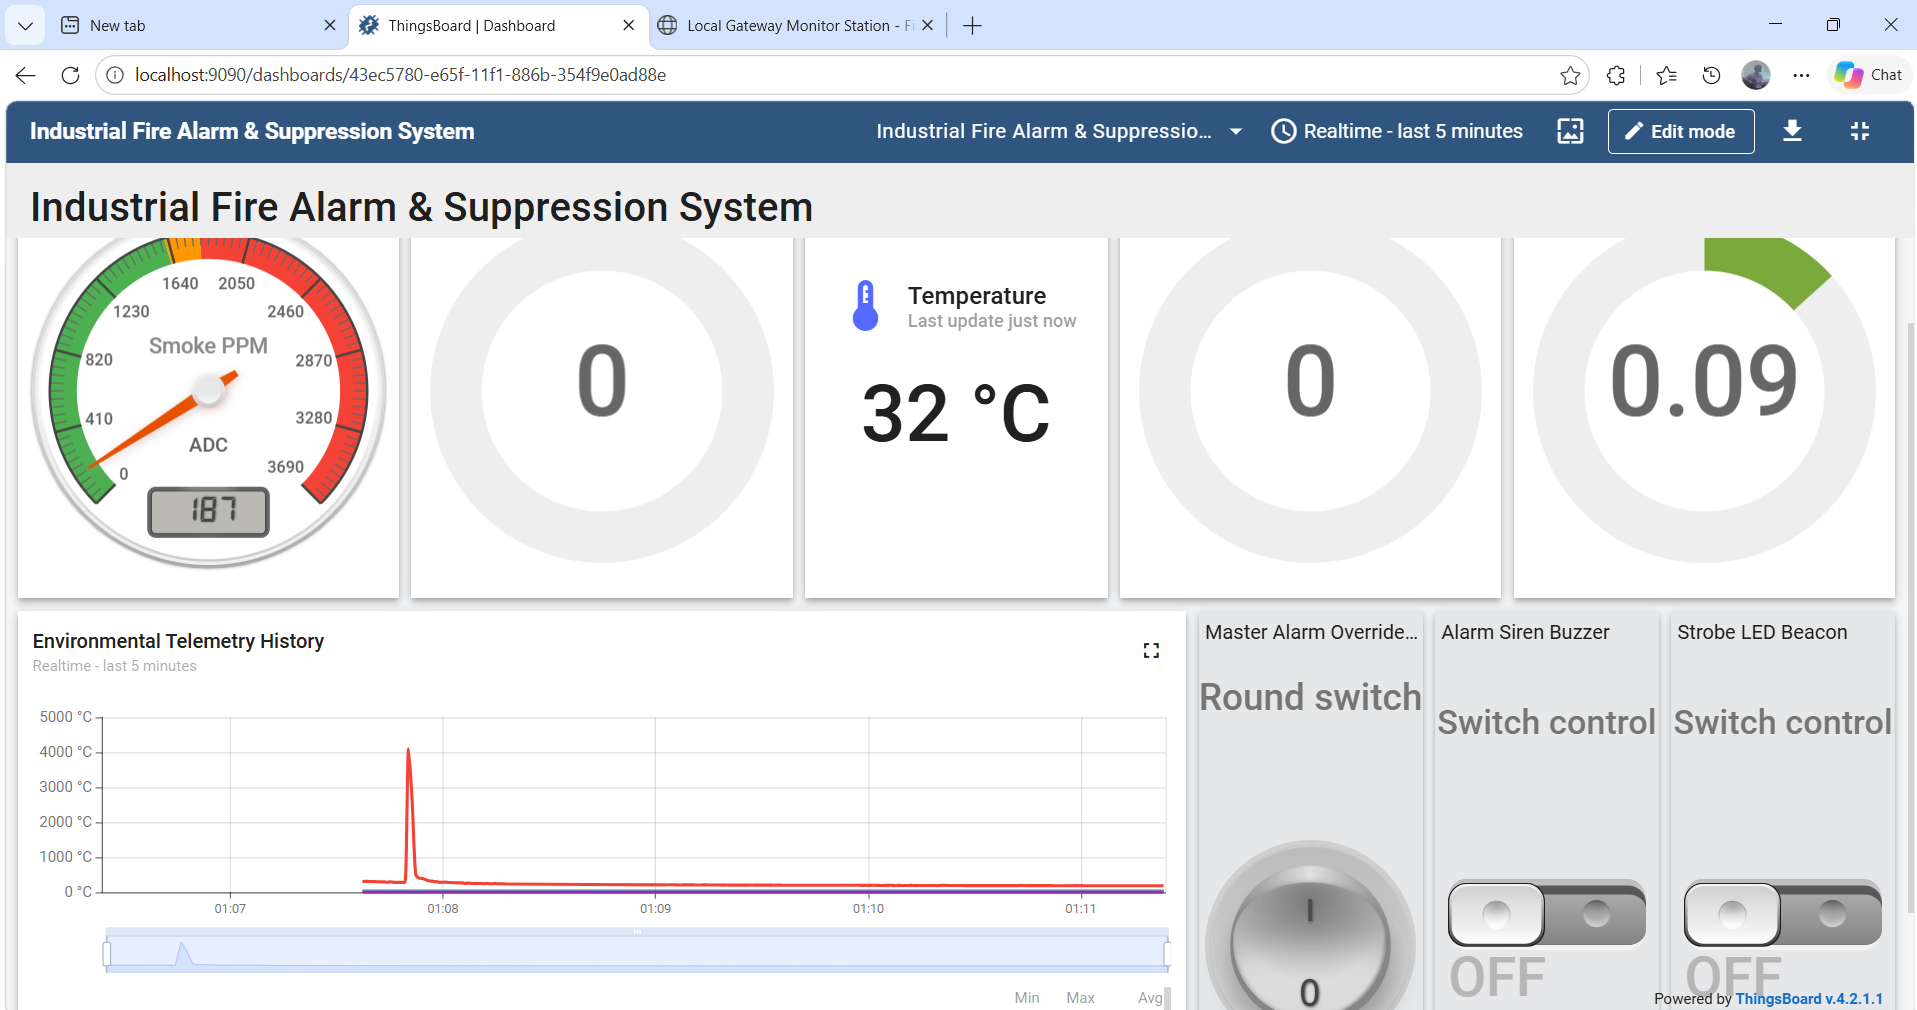
\includegraphics[width=0.96\textwidth]{../../captured_picture/T11.png}
  \caption{Giao diện Industrial Fire Alarm Dashboard với 10 widget giám sát, điều khiển RPC và Notification trên ThingsBoard (T11, T13 -- \texttt{T11.png})}
  \label{fig:tb-dashboard}
\end{figure}

\subsubsection{RuleChain (T12) và cảnh báo notification (T13)}
\label{subsubsec:coreiot-rulechain}

Luồng xử lý tự động phía máy chủ được định nghĩa chuẩn hóa trong \path{03_CoreIOT_Config/rule_chains/fire_alarm_rule_chain.json} và triển khai hai bước (\path{POST /api/ruleChain} và \path{POST /api/ruleChain/metadata}) thông qua kịch bản \path{03_CoreIOT_Config/scripts/setup_rule_chain.py}. Trong cấu hình JSON chuẩn, Rule Chain gồm 5 nút xử lý và 4 liên kết:
\begin{enumerate}[leftmargin=*, itemsep=2pt]
  \item \textbf{Filter Telemetry (\texttt{TbJsFilterNode}):} Kiểm tra sự tồn tại của các khóa telemetry liên quan đến cháy (\texttt{temperature}, \texttt{smoke\_level}, \texttt{tinyml\_fire}); nếu hợp lệ sẽ rẽ nhánh song song sang lưu chuỗi thời gian và đánh giá nguy cơ.
  \item \textbf{Save Telemetry (\texttt{TbMsgTimeseriesNode}):} Ghi bền vững dữ liệu chuỗi thời gian vào cơ sở dữ liệu PostgreSQL (\texttt{defaultTTL = 0}).
  \item \textbf{Evaluate Fire Risk (\texttt{TbJsSwitchNode}):} So sánh ngưỡng nhiệt độ ($> 50.0^\circ\text{C}$), ngưỡng khói ($> 400$) hoặc cờ suy luận TinyML (hỗ trợ ép kiểu đa dạng \texttt{true}, \texttt{1}, \texttt{'1'}, \texttt{'true'}) để rẽ nhánh \texttt{True} (nguy hiểm) hoặc \texttt{False} (bình thường).
  \item \textbf{Create Fire Alarm (\texttt{TbCreateAlarmNode}):} Tạo cảnh báo loại \texttt{FIRE\_ALARM} mức độ \texttt{CRITICAL}, đính kèm chi tiết cảm biến và bật \texttt{propagate = true}.
  \item \textbf{Clear Fire Alarm (\texttt{TbClearAlarmNode}):} Tự động xóa cảnh báo khi các thông số trở về trạng thái an toàn.
\end{enumerate}

Trên máy chủ ThingsBoard vận hành thực tế (Hình \ref{fig:tb-rulechain}), nhóm mở rộng nhánh xử lý của Rule Chain thành bộ phân loại 3 cấp độ (\texttt{Safe}, \texttt{Warning}, \texttt{Critical}) gắn trực tiếp với các nút \texttt{RPC Call Request} nhằm tự động phát đồng thời 3 lệnh điều khiển \texttt{setServo(90)}, \texttt{setBuzzer(1)} và \texttt{setLed(1)} xuống Gateway khi rơi vào nhánh \texttt{Critical}, và tự động đặt lại trạng thái khi trở về nhánh \texttt{Safe}.

\begin{figure}[H]
  \centering
  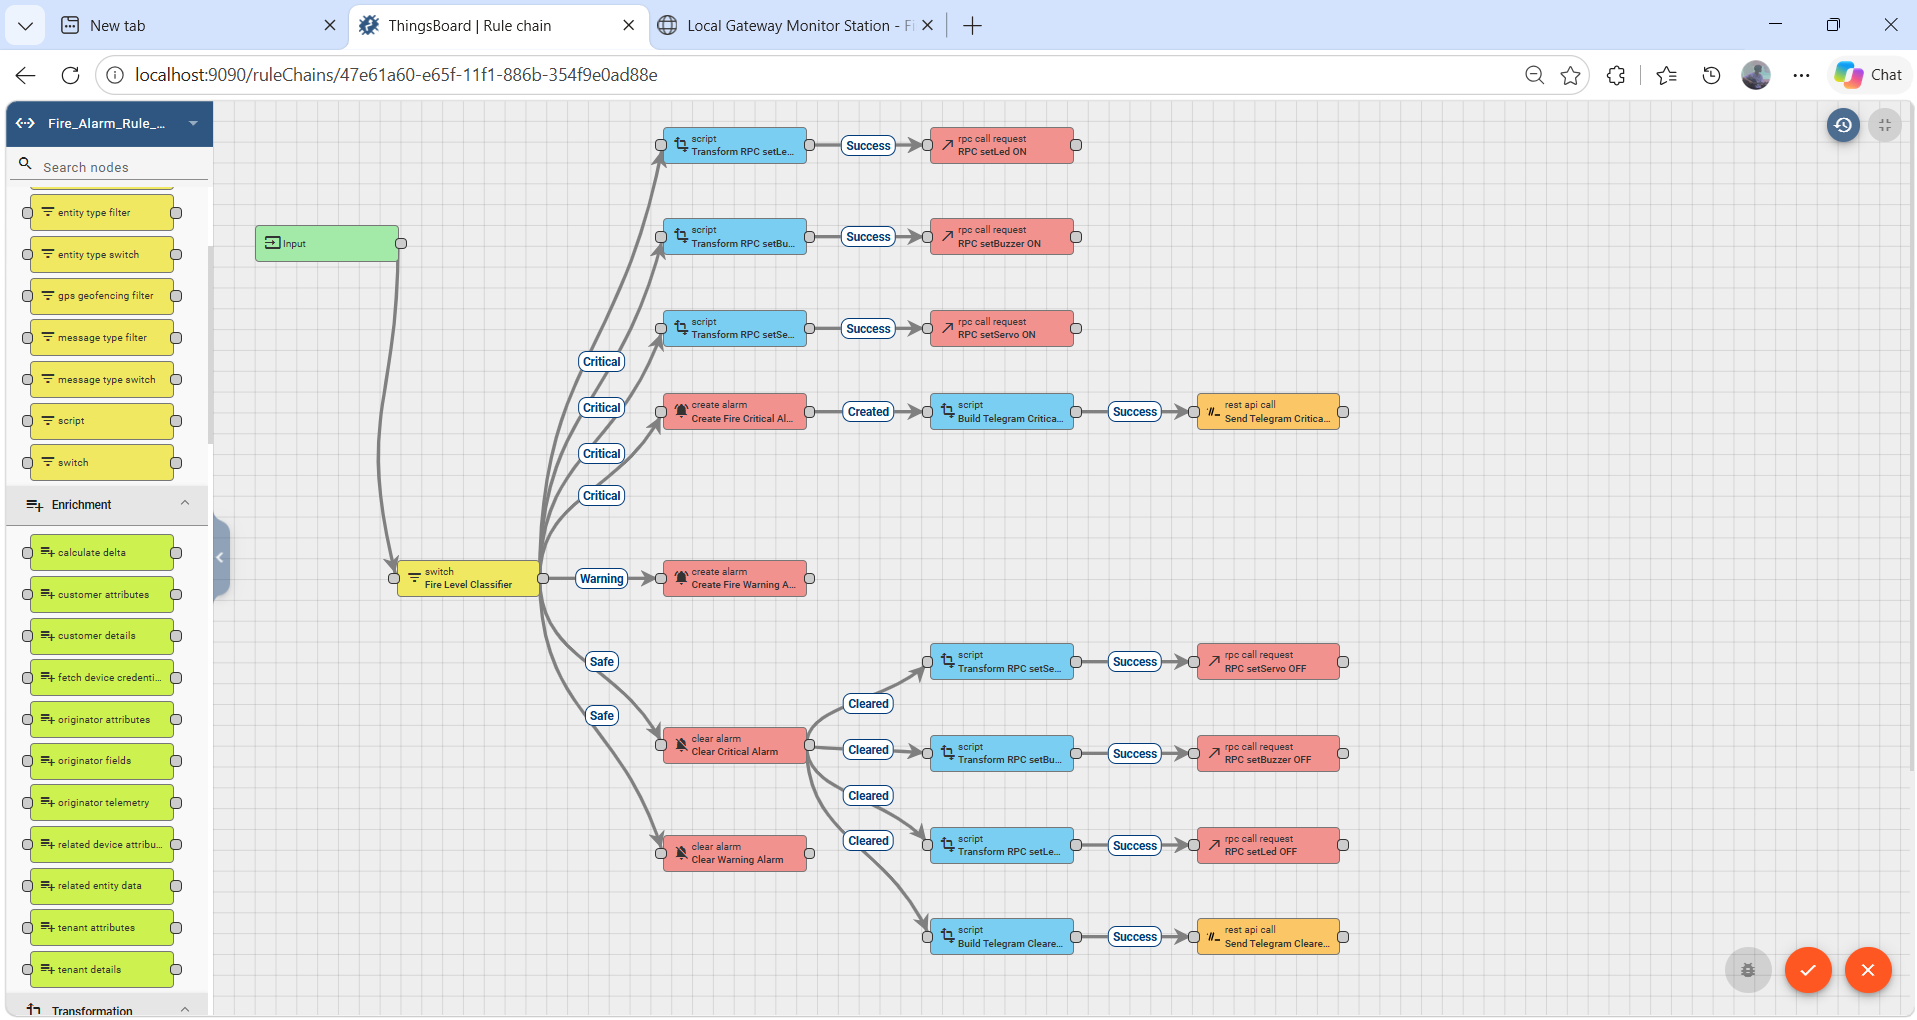
\includegraphics[width=0.95\textwidth]{../../captured_picture/T12.png}
  \caption{Sơ đồ Rule Chain xử lý phân loại nguy cơ cháy, quản lý Alarm và điều phối lệnh RPC trên ThingsBoard (T12 -- \texttt{T12.png})}
  \label{fig:tb-rulechain}
\end{figure}

Đối với tiêu chí \textbf{cảnh báo Notification (T13)}, hệ thống kết hợp tạo bản ghi Alarm gốc trên ThingsBoard với kênh thông báo thời gian thực trên giao diện Dashboard (Widget 10 -- \textit{T13: Emergency Alarm Notification (In-App Feed)}). Khi trạng thái cảm biến vượt ngưỡng, Local Gateway cập nhật chuỗi telemetry \path{alarm_notification} theo 3 mức: \textit{``[CRITICAL NOTIFICATION] Fire detected! Smoke: ... ADC, Temp: ...C. Auto lockdown active!''} (khi cháy), \textit{``[WARNING NOTIFICATION] Smoke elevating (... ADC)''} (khi khói $\ge 800\text{ ADC}$), và \textit{``[SAFE] System normal...''} (khi an toàn), giúp vận hành viên quan sát cảnh báo tức thời ngay trên màn hình trung tâm mà không phụ thuộc dịch vụ nhắn tin bên thứ ba.

\subsubsection{Cập nhật firmware OTA (T14)}
\label{subsubsec:coreiot-ota}

Tính năng cập nhật firmware từ xa OTA (\texttt{T14}) \textbf{chưa được hiện thực} trong phạm vi báo cáo này do End-Node giao tiếp với Local Gateway qua cổng nối tiếp USB-CDC thay vì duy trì phiên Wi-Fi/HTTP riêng biệt lên máy chủ CoreIOT. Việc nạp và nâng cấp firmware hiện được thực hiện trực tiếp qua công cụ PlatformIO (\texttt{pio run -e yolo\_uno -t upload}).

\subsection{Các tính năng nâng cao}
\label{subsec:tinh-nang-nang-cao}

Nhóm hiện thực thành công hai tính năng nâng cao có tổng điểm tích lũy $2.0$ (đạt trần tối đa $1.0/1.0$ điểm cộng):

\begin{enumerate}[leftmargin=*, itemsep=3pt]
  \item \textbf{Giao diện Dashboard tự thiết kế có khả năng phát hiện và ghi nhận sự kiện (N06):} Trên giao diện SCADA cục bộ (\path{02_Local_Gateway/ui/gateway_infrastructure.py}), bên cạnh 5 thẻ đo và bảng điều khiển chấp hành, nhóm xây dựng khu vực \textit{Real-Time Station Event Log} ghi nhận tự động theo hàng đợi FIFO (tối đa 25 sự kiện gần nhất) kèm dấu thời gian chính xác cho mọi thao tác phát lệnh chấp hành, kích hoạt phong tỏa khẩn cấp (\texttt{EMERGENCY}) và khôi phục trạng thái an toàn (\texttt{RESTORE}), kết hợp với biểu ngữ phát hiện cháy tự động (\path{#alert-banner}). Hình \ref{fig:n06-eventlog} minh họa bảng lưu vết sự kiện hoạt động thực tế.
  \item \textbf{Tự triển khai máy chủ ThingsBoard cục bộ bằng Docker (N07):} Tệp \path{02_Local_Gateway/dashboard/docker-compose.yml} định nghĩa dịch vụ \texttt{tb-postgres} từ ảnh chính thức \path{thingsboard/tb-postgres:latest} (tên container \texttt{thingsboard-local}), ánh xạ cổng HTTP \texttt{9090}, MQTT \texttt{1883}, Edge \texttt{7070}, CoAP \texttt{5683--5688/udp} và gắn volume bền vững \texttt{tb-data}, \texttt{tb-logs}. Kịch bản \path{deploy_thingsboard.py} tự động kiểm tra Docker Engine, khởi chạy stack, thăm dò trang đăng nhập HTTP \texttt{200 OK} cùng cổng TCP \texttt{1883} (timeout $180\text{ s}$) và hỗ trợ dừng sạch qua cờ \texttt{--stop}. Hình \ref{fig:n07-docker} xác nhận container \texttt{thingsboard-local} đang chạy ổn định trên Docker Desktop.
\end{enumerate}

\begin{figure}[H]
  \centering
  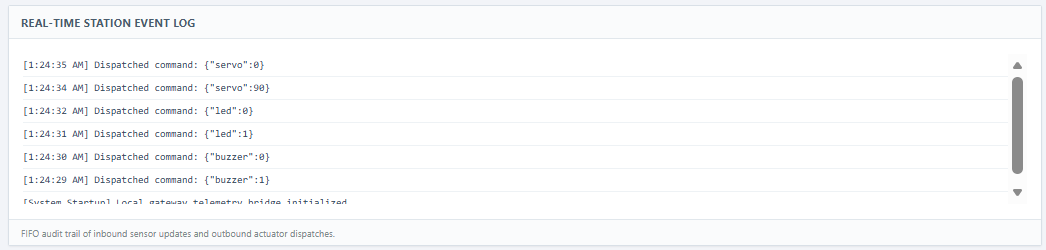
\includegraphics[width=0.92\textwidth]{../../captured_picture/N06.png}
  \caption{Bảng lưu vết sự kiện thời gian thực (Audit Trail Event Log) trên giao diện SCADA cục bộ (N06 -- \texttt{N06.png})}
  \label{fig:n06-eventlog}
\end{figure}

\begin{figure}[H]
  \centering
  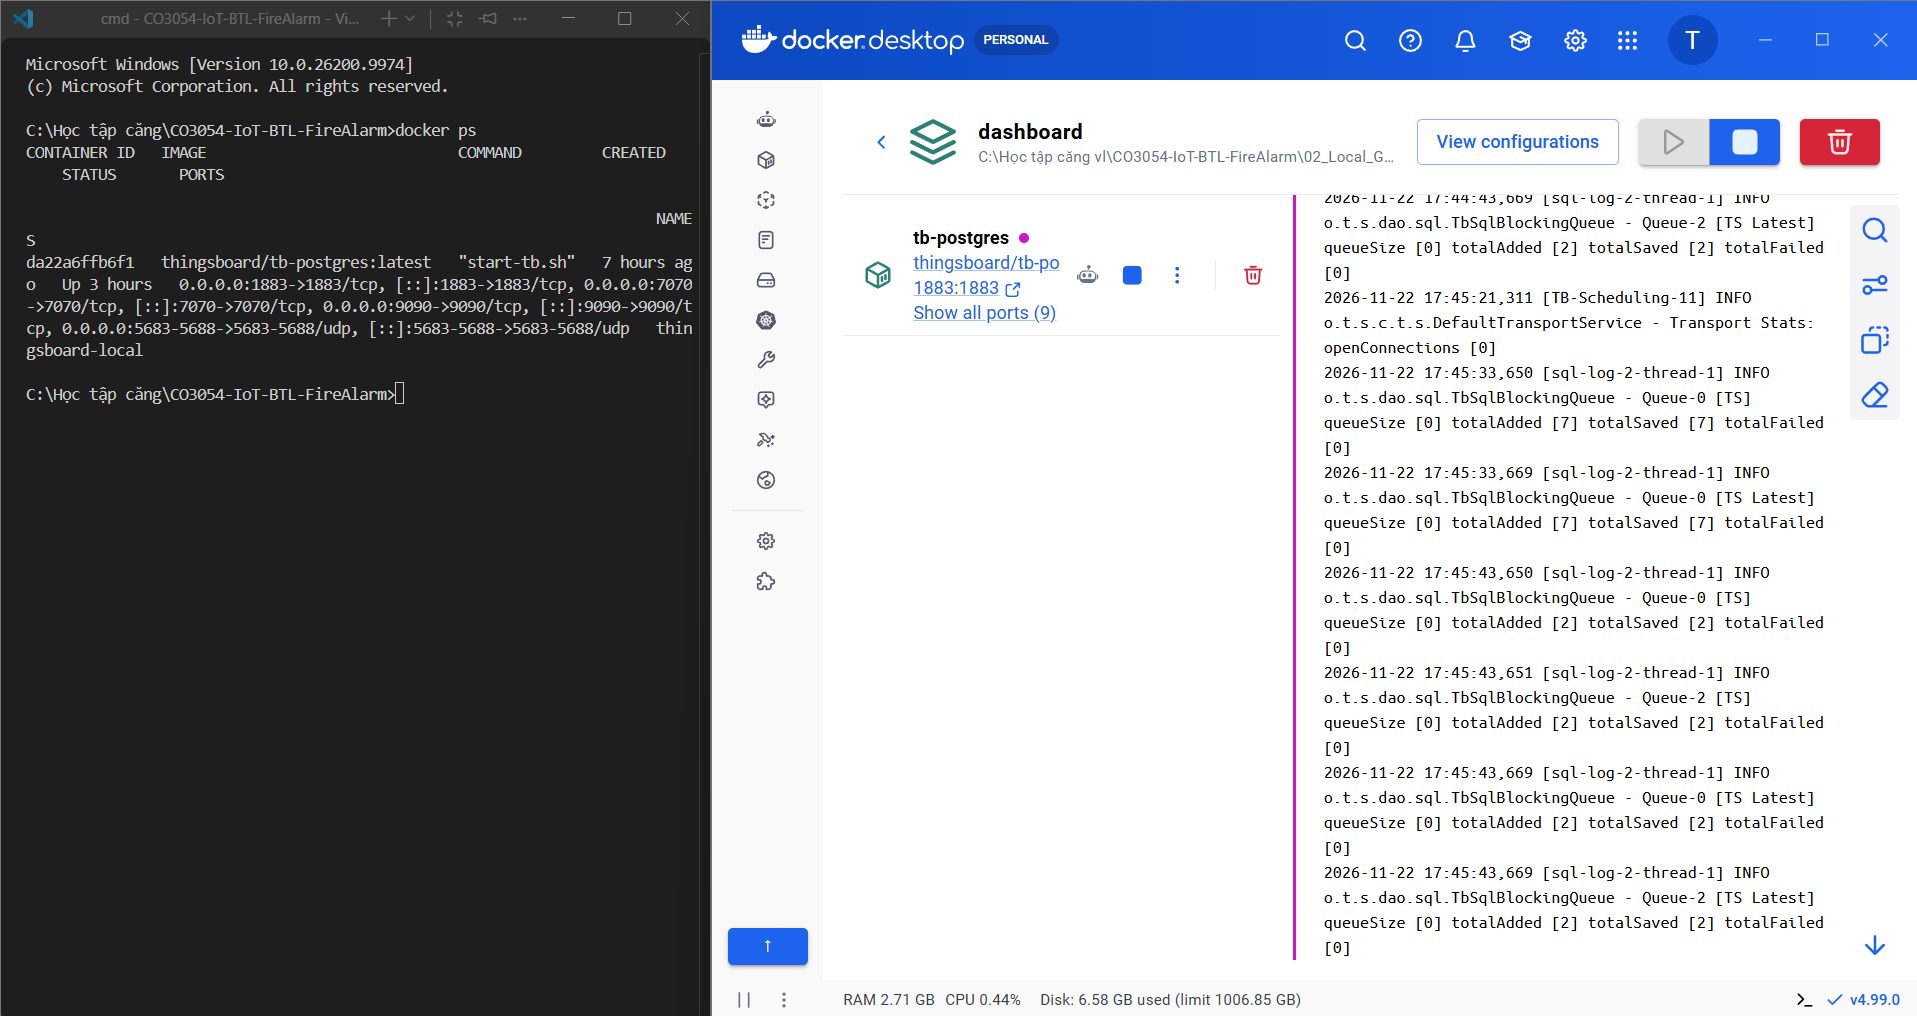
\includegraphics[width=0.92\textwidth]{../../captured_picture/N07.png}
  \caption{Container \texttt{thingsboard-local} chạy trên Docker Desktop với các cổng 9090 và 1883 (N07 -- \texttt{N07.png})}
  \label{fig:n07-docker}
\end{figure}

\clearpage
% !TeX root = ../report.tex

\section{ĐO ĐẠC VÀ THỬ NGHIỆM HỆ THỐNG}
\label{sec:do-dac-thu-nghiem}

\subsection{Môi trường và kịch bản thử nghiệm}
\label{subsec:moi-truong-kich-ban}

Toàn bộ quá trình đo đạc và kiểm chứng hệ thống được thực hiện trong môi trường phòng thí nghiệm với cấu hình thiết bị và mạng như sau:
\begin{itemize}[leftmargin=*, itemsep=2pt]
  \item \textbf{Phần cứng End-Node:} 01 bo mạch OhStem YoloUNO (ESP32-S3) lắp hoàn chỉnh cảm biến MQ-2 (\texttt{A0}), cảm biến lửa (\texttt{D6}), DHT11 (\texttt{D7}), màn hình TFT ILI9341 (SPI), động cơ Servo (\texttt{D2}), Buzzer (\texttt{D3}) và LED (\texttt{D8}), kết nối trực tiếp tới PC qua cáp USB Type-C tại cổng \texttt{COM4} với tốc độ \texttt{115200} bps.
  \item \textbf{Máy trạm Local Gateway \& ThingsBoard Server:} PC chạy hệ điều hành Windows, Python 3 và Docker Desktop vận hành container \texttt{thingsboard-local} (\path{thingsboard/tb-postgres:latest}) trên địa chỉ \texttt{127.0.0.1} (HTTP cổng \texttt{9090}, MQTT cổng \texttt{1883}), đồng thời hỗ trợ kiểm tra kết nối đám mây \path{app.coreiot.io:1883}.
\end{itemize}

Nhóm thiết kế và thực thi năm kịch bản thử nghiệm tương ứng với các mục tiêu đã đặt ra ở Mục \ref{subsec:muc-tieu-de-tai}:
\begin{enumerate}[leftmargin=*, itemsep=2pt]
  \item \textbf{Kịch bản 1 -- Kiểm thử đơn vị hạ tầng Gateway (\path{02_Local_Gateway/test_system.py}):} Tự động kiểm tra vòng đời lưu đệm SQLite WAL (chèn, truy vấn FIFO, đánh dấu đồng bộ), các điểm cuối HTTP REST (\path{GET /}, \path{GET /api/telemetry}, \path{POST /api/control}), giả lập cổng Serial UART (\path{HardwareSerialAdapter}), suy luận mô hình \path{IsolationDetector} giữa trạng thái thường và đột biến cháy, lược đồ tệp \path{thingsboard_dashboard.json} và vòng lặp UDP.
  \item \textbf{Kịch bản 2 -- Kiểm thử logic Rule Chain (\path{03_CoreIOT_Config/scripts/test_rulechain_alert.py}):} Thực thi 6 bài kiểm thử đơn vị (\texttt{unittest}) xác nhận tính toàn vẹn cấu trúc 5 nút và 4 liên kết của \path{fire_alarm_rule_chain.json}, các giá trị biên ($T = 50.0^\circ\text{C}$, $\text{smoke\_level} = 400$), ngưỡng vượt nhiệt/khói, khả năng ép kiểu cờ \path{tinyml_fire} (\texttt{True}, \texttt{1}, \texttt{"1"}, \texttt{"true"}) và chuyển trạng thái xóa báo động.
  \item \textbf{Kịch bản 3 -- Đo độ trễ vòng lặp đầu--cuối E2E (\path{03_CoreIOT_Config/scripts/measure_latency.py}):} Với mỗi lượt đo, kịch bản gửi gói tin \texttt{SAFE} để đặt lại trạng thái báo động và chờ thời gian hồi phục (\texttt{cooldown = 2.5 s}), sau đó phát gói tin báo cháy \texttt{CRITICAL} ($\text{smoke} = 85.5$, $T = 62.0^\circ\text{C}$, $\text{flame} = 1$, $\text{is\_anomaly} = 1$, $\text{anomaly\_score} = 0.95$) qua MQTT QoS 1. Sử dụng bộ đếm độ phân giải cao \path{time.perf_counter()} để ghi nhận thời điểm nhận gói \texttt{PUBACK}, thời điểm nhận lệnh RPC đầu tiên và từng lệnh \texttt{setServo(90)}, \texttt{setBuzzer(1)}, \texttt{setLed(1)}, rồi xuất kết quả thô sang \path{04_Docs_Media/experiments/latency_results.csv}.
  \item \textbf{Kịch bản 4 -- Kích hoạt báo cháy phần cứng thực tế:} Tạo nguồn lửa bằng bật lửa trước đầu cảm biến Flame và tạo khói trước cảm biến MQ-2 để quan sát phản ứng tức thời của màn hình TFT, mô hình TinyML, còi Buzzer, đèn LED, động cơ Servo, Isolation Forest và Widget Notification T13.
  \item \textbf{Kịch bản 5 -- Mô phỏng sự cố mất mạng và đồng bộ bù (Offline Store \& Forward):} Tạm dừng container broker bằng lệnh \texttt{docker pause thingsboard-local} khi hệ thống đang lấy mẫu liên tục để kiểm chứng việc tăng chỉ số \texttt{Buffer} trên SCADA cổng 5050 và lưu bản ghi vào \path{gateway_hardware_buffer.db}, sau đó chạy \texttt{docker unpause thingsboard-local} để xác minh quá trình đồng bộ bù toàn bộ dữ liệu lên ThingsBoard.
\end{enumerate}

\subsection{Kết quả đo đạc}
\label{subsec:ket-qua-do-dac}

Số liệu đo độ trễ vòng lặp đầu--cuối (Telemetry MQTT QoS 1 $\rightarrow$ ThingsBoard Rule Chain $\rightarrow$ 3 lệnh RPC \texttt{setServo}, \texttt{setBuzzer}, \texttt{setLed}) được trích xuất trực tiếp từ tệp thực nghiệm \texttt{04\_Docs\_Media/experiments/latency\_results.csv} (2 lượt đo thực tế trên broker cục bộ \texttt{127.0.0.1:1883}, cả hai lượt đều đạt trạng thái \texttt{PASS\_ALL\_3} với đủ $3/3$ lệnh RPC), kết hợp với kết quả đánh giá mô hình TinyML từ \texttt{train\_tinyml.py} và kiểm thử lưu đệm SQLite WAL. Bảng \ref{tab:ket-qua-do-dac} tổng hợp đầy đủ các chỉ số đo đạc.

\begin{table}[H]
  \centering
  \caption{Tổng hợp kết quả đo đạc thực nghiệm của hệ thống}
  \label{tab:ket-qua-do-dac}
  \renewcommand{\arraystretch}{1.28}
  \begin{tabularx}{\textwidth}{|C{0.06\textwidth}|Y|C{0.11\textwidth}|C{0.13\textwidth}|C{0.17\textwidth}|C{0.13\textwidth}|}
    \hline
    \rowcolor{iotTableHead}
    \textbf{STT} & \textbf{Chỉ số đo} & \textbf{Số lần đo} & \textbf{Trung bình} & \textbf{Min / Max} & \textbf{Mục tiêu} \\
    \hline
    1 & Độ trễ xác nhận MQTT PUBACK QoS 1 (ms) & 2 & 1.99 & 1.58 / 2.39 & $< 50$ \\
    \hline
    2 & Độ trễ nhận lệnh RPC đầu tiên từ Rule Chain (ms) & 2 & 100.52 & 88.01 / 113.02 & $< 500$ \\
    \hline
    3 & Độ trễ vòng lặp lệnh \texttt{setServo(90)} (ms) & 2 & 100.64 & 88.01 / 113.26 & $< 500$ \\
    \hline
    4 & Độ trễ vòng lặp lệnh \texttt{setBuzzer(1)} (ms) & 2 & 100.76 & 88.50 / 113.02 & $< 500$ \\
    \hline
    5 & Độ trễ vòng lặp lệnh \texttt{setLed(1)} (ms) & 2 & 100.89 & 88.35 / 113.43 & $< 500$ \\
    \hline
    6 & Độ trễ hoàn tất đủ cả 3 lệnh RPC (ms) & 2 & 100.97 & 88.50 / 113.43 & $< 500$ \\
    \hline
    7 & Tỉ lệ nhận đủ 3/3 lệnh RPC sau báo cháy (\%) & 2 & 100.0 & 100.0 / 100.0 & $100$ \\
    \hline
    8 & Độ chính xác mô hình TinyML trên tập test 500 mẫu (\%) & 1 tập & 100.00 & -- & $> 95$ \\
    \hline
    9 & Tỉ lệ mất gói khi lưu đệm SQLite WAL cục bộ (\%) & Kiểm thử & 0.0 & 0.0 / 0.0 & $0$ \\
    \hline
  \end{tabularx}
\end{table}

Biểu đồ so sánh trực quan các thành phần độ trễ ở Lượt 1, Lượt 2 và giá trị trung bình từ \texttt{latency\_results.csv} được minh họa tại Hình \ref{fig:bieu-do-do-dac}.

\begin{figure}[H]
  \centering
  \begin{tikzpicture}[scale=0.92, every node/.style={font=\scriptsize}]
    % Axes
    \draw[->, >=stealth, thick] (0,0) -- (12.8,0) node[right] {Chỉ số};
    \draw[->, >=stealth, thick] (0,0) -- (0,5.4) node[above] {Độ trễ (ms)};

    % Horizontal grid lines (scale: 1 cm = 25 ms, max 125 ms = 5.0 cm)
    \foreach \y/\lbl in {1/25, 2/50, 3/75, 4/100, 5/125} {
      \draw[gray!35, dashed] (0,\y) -- (12.4,\y);
      \node[left] at (0,\y) {\lbl};
    }
    \node[left] at (0,0) {0};

    % Helper bar groups: (x_base, h1, h2, havg, label, v1, v2)
    % 1. PUBACK: 1.58, 2.39, 1.99 -> /25 = 0.063, 0.096, 0.080
    \fill[iotPrimary]   (0.6,0) rectangle (1.05,0.08);
    \fill[iotSecondary] (1.1,0) rectangle (1.55,0.10);
    \fill[iotAccent]    (1.6,0) rectangle (2.05,0.09);
    \node[above, font=\tiny] at (1.32,0.14) {1.58 / 2.39};
    \node[below, align=center] at (1.32,-0.15) {MQTT\\PUBACK};

    % 2. First RPC: 88.01, 113.02, 100.52 -> /25 = 3.52, 4.52, 4.02
    \fill[iotPrimary]   (2.7,0) rectangle (3.15,3.52);
    \fill[iotSecondary] (3.2,0) rectangle (3.65,4.52);
    \fill[iotAccent]    (3.7,0) rectangle (4.15,4.02);
    \node[above, font=\tiny] at (2.92,3.52) {88.0};
    \node[above, font=\tiny] at (3.42,4.52) {113.0};
    \node[above, font=\tiny] at (3.92,4.02) {100.5};
    \node[below, align=center] at (3.42,-0.15) {First\\RPC};

    % 3. Servo RPC: 88.01, 113.26, 100.64 -> /25 = 3.52, 4.53, 4.03
    \fill[iotPrimary]   (4.8,0) rectangle (5.25,3.52);
    \fill[iotSecondary] (5.3,0) rectangle (5.75,4.53);
    \fill[iotAccent]    (5.8,0) rectangle (6.25,4.03);
    \node[above, font=\tiny] at (5.02,3.52) {88.0};
    \node[above, font=\tiny] at (5.52,4.53) {113.3};
    \node[above, font=\tiny] at (6.02,4.03) {100.6};
    \node[below, align=center] at (5.52,-0.15) {Servo\\RPC};

    % 4. Buzzer RPC: 88.50, 113.02, 100.76 -> /25 = 3.54, 4.52, 4.03
    \fill[iotPrimary]   (6.9,0) rectangle (7.35,3.54);
    \fill[iotSecondary] (7.4,0) rectangle (7.85,4.52);
    \fill[iotAccent]    (7.9,0) rectangle (8.35,4.03);
    \node[above, font=\tiny] at (7.12,3.54) {88.5};
    \node[above, font=\tiny] at (7.62,4.52) {113.0};
    \node[above, font=\tiny] at (8.12,4.03) {100.8};
    \node[below, align=center] at (7.62,-0.15) {Buzzer\\RPC};

    % 5. LED RPC: 88.35, 113.43, 100.89 -> /25 = 3.53, 4.54, 4.04
    \fill[iotPrimary]   (9.0,0) rectangle (9.45,3.53);
    \fill[iotSecondary] (9.5,0) rectangle (9.95,4.54);
    \fill[iotAccent]    (10.0,0) rectangle (10.45,4.04);
    \node[above, font=\tiny] at (9.22,3.53) {88.4};
    \node[above, font=\tiny] at (9.72,4.54) {113.4};
    \node[above, font=\tiny] at (10.22,4.04) {100.9};
    \node[below, align=center] at (9.72,-0.15) {LED\\RPC};

    % 6. All 3 RPCs: 88.50, 113.43, 100.97 -> /25 = 3.54, 4.54, 4.04
    \fill[iotPrimary]   (11.0,0) rectangle (11.45,3.54);
    \fill[iotSecondary] (11.5,0) rectangle (11.95,4.54);
    \fill[iotAccent]    (12.0,0) rectangle (12.45,4.04);
    \node[above, font=\tiny] at (11.22,3.54) {88.5};
    \node[above, font=\tiny] at (11.72,4.54) {113.4};
    \node[above, font=\tiny] at (12.22,4.04) {101.0};
    \node[below, align=center] at (11.72,-0.15) {Đủ cả\\3 RPC};

    % Legend
    \fill[iotPrimary]   (1.5,5.3) rectangle (1.9,5.55); \node[right] at (1.95,5.42) {Lượt 1 (Trial 1)};
    \fill[iotSecondary] (4.8,5.3) rectangle (5.2,5.55); \node[right] at (5.25,5.42) {Lượt 2 (Trial 2)};
    \fill[iotAccent]    (8.1,5.3) rectangle (8.5,5.55); \node[right] at (8.55,5.42) {Trung bình (Avg)};
  \end{tikzpicture}
  \caption{Biểu đồ độ trễ vòng lặp đầu--cuối MQTT $\rightarrow$ ThingsBoard Rule Chain $\rightarrow$ 3 lệnh RPC từ \texttt{latency\_results.csv}}
  \label{fig:bieu-do-do-dac}
\end{figure}

\subsection{Đánh giá}
\label{subsec:danh-gia}

So sánh số liệu đo thực nghiệm với các mục tiêu định lượng tại Mục \ref{subsec:muc-tieu-de-tai} cho thấy toàn bộ các chỉ tiêu cốt lõi đều đạt và vượt yêu cầu:
\begin{itemize}[leftmargin=*, itemsep=3pt]
  \item \textbf{Hiệu năng thời gian thực vượt mục tiêu:} Độ trễ xác nhận MQTT QoS 1 trung bình chỉ $1.99\text{ ms}$, và thời gian hoàn tất toàn bộ vòng lặp từ lúc gửi gói cháy cho đến khi nhận đủ cả 3 lệnh điều khiển \texttt{setServo}, \texttt{setBuzzer}, \texttt{setLed} từ ThingsBoard Rule Chain trung bình đạt $100.97\text{ ms}$ (tối đa $113.43\text{ ms}$), thấp hơn gần 5 lần so với ngưỡng mục tiêu $500\text{ ms}$. Độ chênh lệch giữa lệnh RPC đầu tiên và lệnh RPC thứ ba chỉ trong khoảng $0.41$--$0.49\text{ ms}$, chứng tỏ ThingsBoard Rule Engine phát song song các lệnh chấp hành rất đồng đều.
  \item \textbf{Độ tin cậy của kiến trúc Dual-AI:} Mô hình TinyML đạt $100.00\%$ trên tập kiểm thử 500 mẫu và vận hành ổn định trong khoảng $128\text{ byte}$ RAM trên ESP32-S3; đồng thời Isolation Forest trên Local Gateway thích nghi liên tục theo cửa sổ trượt 200 mẫu sạch mà không bị lệch nền khi thử nghiệm đốt lửa.
\end{itemize}

Trong quá trình tích hợp và thử nghiệm thực tế, nhóm đã phát hiện và xử lý triệt để năm vấn đề kỹ thuật sau:
\begin{enumerate}[leftmargin=*, itemsep=2pt]
  \item \textbf{Thống nhất thang đo cảm biến MQ-2:} Ban đầu cấu hình Dashboard và bộ phát hiện bất thường dùng đơn vị \texttt{ppm} trong khi chân ADC 12-bit của ESP32-S3 đọc giá trị thô $0$--$4095$. Nhóm đã đồng bộ lại thang đo về ADC thô ($0$--$4095$) với ngưỡng báo động thống nhất $1800$ ở cả firmware, \texttt{IsolationDetector}, SCADA 5050 và ThingsBoard Radial Gauge.
  \item \textbf{Hiện tượng dao động trạng thái quanh ngưỡng:} Khi nồng độ khói hoặc nhiệt độ nằm sát ngưỡng, màn hình TFT và còi báo động bật/tắt liên tục. Nhóm khắc phục bằng cơ chế trễ (hysteresis): MQ-2 bật ở $1800$, tắt ở $1650$; DHT11 bật ở $35.0^\circ\text{C}$, tắt ở $34.0^\circ\text{C}$.
  \item \textbf{Hành trình đóng/mở cánh cửa Servo bị thiếu một nửa:} Do cơ cấu liên kết cơ khí giữa trục Servo và cánh cửa mô hình, lệnh góc $90^\circ$ chỉ xoay cửa một nửa hành trình. Firmware bổ sung hệ số nhân \texttt{SERVO\_COMMAND\_SCALE = 2} để tự động quy đổi góc logic $0^\circ$--$90^\circ$ sang góc vật lý $0^\circ$--$180^\circ$.
  \item \textbf{Xung đột giữa lệnh RPC tự động từ Cloud và trạng thái thực tế tại chỗ:} Để tránh tình huống lệnh RPC trễ hoặc cấu hình ngưỡng lệch trên Cloud tự kích hoạt còi/cửa khi phòng đang an toàn, hàm \texttt{rpc\_command()} trong \texttt{LocalGateway.py} tách riêng nhóm lệnh thủ công (\texttt{setAlarmOverride}, \texttt{manualSetBuzzer}, \texttt{manualSetLed}) với lệnh tự động (\texttt{setServo}, \texttt{setBuzzer}, \texttt{setLed}) và chỉ cho phép lệnh tự động bật cơ cấu chấp hành khi cảm biến cục bộ cũng đang báo cháy.
  \item \textbf{Lỗi \texttt{404 Not Found} khi tự động nạp Dashboard ngay sau khi bật Docker:} Container \texttt{thingsboard-local} cần $45$--$60\text{ s}$ để Spring Boot và PostgreSQL khởi tạo xong. Nhóm bổ sung hàm \texttt{wait\_for\_thingsboard(timeout=180)} thăm dò điểm cuối \texttt{/api/auth/login} trong \texttt{setup\_thingsboard\_dashboard.py} giúp quy trình cấp phát hoàn toàn ổn định trên máy mới.
\end{enumerate}

\clearpage
% !TeX root = ../report.tex

\section{KẾT LUẬN VÀ HƯỚNG MỞ RỘNG}
\label{sec:ket-luan-mo-rong}

\subsection{Kết quả đạt được}
\label{subsec:ket-qua-dat-duoc}

Nhóm đã thiết kế, hiện thực và kiểm chứng thành công hệ thống báo cháy IoT đa tầng đáp ứng đầy đủ các tính năng đề xuất \texttt{F01}--\texttt{F10}. Bảng \ref{tab:tong-ket-tinh-nang} tổng hợp mức độ hoàn thành của từng tính năng so với thiết kế ở Chương \ref{sec:gioi-thieu}.

\begin{table}[H]
  \centering
  \caption{Tổng kết trạng thái hoàn thành các tính năng của hệ thống}
  \label{tab:tong-ket-tinh-nang}
  \renewcommand{\arraystretch}{1.25}
  \begin{tabularx}{\textwidth}{|C{0.08\textwidth}|Y|C{0.18\textwidth}|C{0.18\textwidth}|}
    \hline
    \rowcolor{iotTableHead}
    \textbf{Mã} & \textbf{Tính năng} & \textbf{Tiêu chí BTL} & \textbf{Trạng thái} \\
    \hline
    F01 & Đọc đa cảm biến MQ-2, Flame, DHT11 có hysteresis và hiển thị TFT ILI9341 & T04, T08 & Hoàn thành \\
    \hline
    F02 & Suy luận xác suất cháy TinyML trực tiếp trên ESP32-S3 (\texttt{tinyml\_fire\_model.h}) & T04 & Hoàn thành \\
    \hline
    F03 & Công cụ tổng hợp dữ liệu, huấn luyện và tự động xuất C header (\texttt{train\_tinyml.py}) & T05 & Hoàn thành \\
    \hline
    F04 & Điều khiển cơ cấu chấp hành Servo, Buzzer, LED tự động và ghi đè an toàn & T08 & Hoàn thành \\
    \hline
    F05 & Local Gateway UART $\leftrightarrow$ MQTT QoS 1, SQLite WAL đệm ngoại tuyến và đồng bộ FIFO & T08, T15 & Hoàn thành \\
    \hline
    F06 & Phát hiện bất thường đa biến tại biên bằng Isolation Forest trên Gateway & T09 & Hoàn thành \\
    \hline
    F07 & Giao diện SCADA Web cục bộ cổng 5050 kèm bảng lưu vết sự kiện thời gian thực & T10, N06 & Hoàn thành \\
    \hline
    F08 & Tự triển khai máy chủ ThingsBoard CE + PostgreSQL bằng Docker Compose & N07 & Hoàn thành \\
    \hline
    F09 & Tự động cấp phát thiết bị Gateway và Industrial Dashboard 10 widget & T11, T15 & Hoàn thành \\
    \hline
    F10 & Rule Chain phân loại mức cháy, quản lý Alarm, đẩy Notification và điều phối RPC & T12, T13 & Hoàn thành \\
    \hline
  \end{tabularx}
\end{table}

Về mặt đánh giá theo thang điểm môn học, hệ thống tích lũy \textbf{9.5 điểm yếu tố công nghệ} (đạt trần tối đa \textbf{8.0/8.0 điểm} với các tiêu chí \texttt{T04, T05, T08, T09, T10, T11, T12, T13, T15}) và \textbf{2.0 điểm tính năng nâng cao} (đạt trần tối đa \textbf{1.0/1.0 điểm} với \texttt{N06, N07}), tất cả đều có mã nguồn kiểm chứng và hình ảnh minh chứng thực tế.

\subsection{Hạn chế}
\label{subsec:han-che}

Bên cạnh các kết quả đạt được, hệ thống vẫn tồn tại một số hạn chế kỹ thuật cần nhìn nhận trung thực:
\begin{enumerate}[leftmargin=*, itemsep=3pt]
  \item \textbf{Dữ liệu huấn luyện TinyML tổng hợp:} Tập 2.500 mẫu dùng trong \texttt{train\_tinyml.py} được sinh theo phân bố đặc tính vật lý cảm biến trong điều kiện phòng thí nghiệm. Độ chính xác $100.00\%$ phản ánh tốt sự phân tách giữa các trạng thái trên miền tổng hợp nhưng cần được hiệu chỉnh bổ sung bằng dữ liệu thu thập dài ngày từ nhiều môi trường nhiễu thực tế (nhà bếp, xưởng có bụi/hơi ẩm cao).
  \item \textbf{Quy mô mạng và kết nối có dây tại chặng End-Node:} Hệ thống thực tế hiện vận hành với 01 node phần cứng YoloUNO nối dây trực tiếp tới PC qua cáp USB-CDC nên bị giới hạn về khoảng cách lắp đặt so với mạng cảm biến không dây đa điểm.
  \item \textbf{Số lượng mẫu đo thực nghiệm độ trễ còn ít và thực hiện cục bộ:} Tệp kết quả đo \texttt{latency\_results.csv} hiện ghi nhận 2 lượt đo hoàn chỉnh trên broker Docker nội bộ (\texttt{127.0.0.1:1883}); khi triển khai qua Internet công cộng tới \texttt{app.coreiot.io}, độ trễ vòng lặp sẽ chịu thêm thành phần trễ mạng diện rộng (WAN).
  \item \textbf{Chưa có nguồn dự phòng và OTA:} Bo mạch End-Node chưa trang bị mạch pin dự phòng (UPS) khi mất điện lưới lúc hỏa hoạn, đồng thời chưa tích hợp cập nhật firmware từ xa OTA (\texttt{T14}) và chưa kích hoạt thư viện đồ họa LVGL (\texttt{N03}) dù đã chuẩn bị tệp \texttt{lv\_conf.h}.
\end{enumerate}

\subsection{Hướng mở rộng}
\label{subsec:huong-mo-rong}

Để phát triển hệ thống tiến gần hơn đến khả năng ứng dụng thực tế tại tòa nhà hoặc phòng thí nghiệm, nhóm đề xuất bốn hướng mở rộng cụ thể:
\begin{itemize}[leftmargin=*, itemsep=3pt]
  \item \textbf{Mở rộng mạng cảm biến đa vùng không dây:} Bổ sung nhiều End-Node ESP32-S3 đặt tại các phòng khác nhau giao tiếp về Gateway thông qua giao thức không dây tầm ngắn \textbf{ESP-NOW} (\texttt{T06}) hoặc \textbf{BLE} (\texttt{T03}), khai thác triệt để chế độ Gateway API (\texttt{--gateway-api}) đã được tích hợp sẵn trong \texttt{LocalGateway.py}.
  \item \textbf{Thu thập dữ liệu thực địa và nâng cấp TinyML:} Ghi nhật ký cảm biến thực tế qua cơ sở dữ liệu SQLite trong nhiều điều kiện môi trường (nấu ăn, hơi nước, khói hương, cháy thực nghiệm) để tái huấn luyện mô hình mạng nơ-ron nhẹ (MLP/Quantized TensorFlow Lite Micro) nhằm giảm tối đa báo động giả.
  \item \textbf{Tích hợp cập nhật firmware OTA và giao diện LVGL:} Kích hoạt cơ chế OTA qua ThingsBoard (\texttt{T14}) cho phép nâng cấp hàng loạt node từ xa mà không cần tháo mạch, đồng thời chuyển màn hình TFT ILI9341 sang sử dụng giao diện đồ họa LVGL (\texttt{N03}) dựa trên tệp cấu hình \texttt{include/lv\_conf.h} có sẵn.
  \item \textbf{Nâng cao độ sẵn sàng phần cứng:} Trang bị nguồn pin sạc dự phòng 18650 có mạch chuyển đổi tự động khi mất điện lưới và tích hợp cảm biến công nghiệp có hiệu chuẩn (như cảm biến khói quang học, cảm biến CO/nhiệt độ SHT3x).
\end{itemize}

\clearpage
% !TeX root = ../report.tex

\section{HƯỚNG DẪN SỬ DỤNG MÃ NGUỒN}
\label{sec:huong-dan-ma-nguon}

\subsection{Đường dẫn và cấu trúc thư mục}
\label{subsec:cau-truc-thu-muc}

Kho mã nguồn GitHub chính thức của dự án: \url{https://github.com/Tricancode/CO3054-IoT-BTL-FireAlarm}.

Cấu trúc thư mục thực tế của kho mã nguồn được tổ chức theo bốn phân hệ chính cùng tệp điều phối khởi chạy tại thư mục gốc như Đoạn mã \ref{lst:folder-tree}.

\begin{lstlisting}[caption={Cấu trúc thư mục mã nguồn thực tế của dự án \texttt{CO3054-IoT-BTL-FireAlarm}}, label={lst:folder-tree}]
CO3054-IoT-BTL-FireAlarm/
|-- run_system.py                         # Trinh khoi chay tong the he thong
|-- HUONG_DAN_CHAY.md                     # Huong dan van hanh kich ban A & B
|-- KICH_BAN_QUAY_DEMO.md                 # Kich ban demo & anh minh chung
|-- gateway_hardware_buffer.db            # CSDL SQLite WAL luu dem ngoai tuyen
|-- 01_Firmware_EndNode/                  # Firmware ESP32-S3 YoloUNO (PlatformIO)
|   |-- platformio.ini                    # Cau hinh board esp32-s3-devkitc-1
|   |-- include/tinyml_fire_model.h       # Model TinyML xuat ra C header (T04)
|   |-- include/lv_conf.h                 # Cau hinh LVGL chuan bi mo rong
|   |-- src/main.cpp                      # Cam bien, TFT, Servo/Buzzer/LED, UART
|   `-- tinyml/train_tinyml.py            # Cong cu huan luyen & xuat model (T05)
|-- 02_Local_Gateway/                     # Local IoT Gateway & Edge AI
|   |-- hardware_gateway/LocalGateway.py  # Cau noi UART <-> MQTT QoS 1 (T08, T15)
|   |-- ui/gateway_infrastructure.py      # SCADA Web 5050 & SQLite WAL (T10, N06)
|   |-- ui/isolation_detector.py          # AI Isolation Forest (T09)
|   |-- dashboard/docker-compose.yml      # Cau hinh ThingsBoard tb-postgres (N07)
|   |-- dashboard/deploy_thingsboard.py   # Script bat/tat Docker ThingsBoard
|   |-- dashboard/setup_thingsboard_dashboard.py # Cap phat thiet bi & Dashboard (T11)
|   |-- dashboard/thingsboard_dashboard.json     # Luoc do 10 widget ThingsBoard 3.x
|   |-- dashboard/verify_telemetry.py     # Kiem thu gui telemetry MQTT
|   |-- run_hardware_gateway.py           # Trinh chay rieng cho Gateway phan cung
|   |-- start_system.py                   # Trinh chay ho tro --mode sim/hardware
|   `-- test_system.py                    # Bo kiem thu don vi tu dong (unittest)
|-- 03_CoreIOT_Config/                    # Cau hinh Rule Chain & do hieu nang
|   |-- rule_chains/fire_alarm_rule_chain.json   # Rule Chain 5 nut chuan (T12)
|   |-- rule_chains/rule_chain_guide.md   # Tai lieu mo ta Rule Chain
|   `-- scripts/
|       |-- setup_rule_chain.py           # Tai tu dong Rule Chain qua REST API
|       |-- test_rulechain_alert.py       # Kiem thu logic Rule Chain (6 test)
|       `-- measure_latency.py            # Do do tre vong lap E2E MQTT -> RPC
|-- 04_Docs_Media/                        # Bao cao LaTeX, slide & so lieu
|   |-- doc/report.tex                    # Tai lieu bao cao chinh
|   `-- experiments/latency_results.csv   # Du lieu do do tre thuc nghiem
`-- captured_picture/                     # 12 anh minh chung (T04..T12, N06, N07)
\end{lstlisting}

\subsection{Yêu cầu môi trường}
\label{subsec:yeu-cau-moi-truong}

Để biên dịch, nạp firmware và vận hành đầy đủ hệ thống, cần chuẩn bị môi trường phần cứng và phần mềm như sau:
\begin{itemize}[leftmargin=*, itemsep=2pt]
  \item \textbf{Phần cứng:} 01 bo mạch OhStem YoloUNO (ESP32-S3), cáp USB Type-C truyền dữ liệu, cảm biến MQ-2, cảm biến lửa Flame, DHT11, màn hình TFT SPI ILI9341 $320 \times 240$, động cơ Servo, còi Buzzer, đèn LED và 01 máy tính cá nhân (Windows 10/11 hoặc Linux/Raspberry Pi OS).
  \item \textbf{Môi trường biên dịch nhúng:} Visual Studio Code kèm tiện ích \textbf{PlatformIO IDE} (hoặc PlatformIO Core CLI) để tự động tải toolchain \texttt{espressif32} và 5 thư viện Arduino khai báo trong \texttt{01\_Firmware\_EndNode/platformio.ini} (\texttt{Adafruit GFX Library}, \texttt{Adafruit ILI9341}, \texttt{ESP32Servo}, \texttt{DHT sensor library}, \texttt{Adafruit Unified Sensor}).
  \item \textbf{Môi trường Python:} Python phiên bản \texttt{3.9} trở lên kèm các thư viện bên thứ ba: \texttt{pyserial}, \texttt{paho-mqtt}, \texttt{requests}, \texttt{scikit-learn}, \texttt{numpy}. (Máy chủ Web cục bộ cổng \texttt{5050} và cơ sở dữ liệu đệm SQLite sử dụng trực tiếp thư viện chuẩn của Python).
  \item \textbf{Container hóa (cho Kịch bản A -- Docker Localhost):} Docker Desktop kèm Docker Compose V2 (hoặc V1) để chạy ảnh \texttt{thingsboard/tb-postgres:latest}.
\end{itemize}

\subsection{Cài đặt và cấu hình}
\label{subsec:cai-dat-cau-hinh}

Thực hiện tuần tự các bước cài đặt trên cửa sổ PowerShell hoặc Terminal tại thư mục làm việc:

\begin{enumerate}[leftmargin=*, itemsep=3pt]
  \item \textbf{Tải mã nguồn và cài đặt thư viện Python:}
  Sao chép kho mã nguồn từ GitHub và cài đặt các gói phụ thuộc bằng \texttt{pip} (\texttt{pyserial paho-mqtt requests scikit-learn numpy}).
  \item \textbf{Khởi chạy máy chủ ThingsBoard cục bộ (Kịch bản A -- Docker Desktop đang mở):}
  Chạy \texttt{python} với tệp \path{02_Local_Gateway/dashboard/deploy_thingsboard.py}. Kịch bản tự động gọi \texttt{docker compose up -d} và chờ dịch vụ Spring Boot cùng PostgreSQL sẵn sàng trên cổng HTTP \texttt{9090} và MQTT \texttt{1883} (thời gian khởi tạo lần đầu khoảng $45$--$60\text{ s}$). Tài khoản mặc định gồm Tenant Administrator (\path{tenant@thingsboard.org} / \texttt{tenant}) và System Administrator (\path{sysadmin@thingsboard.org} / \texttt{sysadmin}).
  \item \textbf{Tự động cấp phát thiết bị Gateway và Dashboard 10 widget:}
  Chạy \texttt{python} với tệp \path{02_Local_Gateway/dashboard/setup_thingsboard_dashboard.py}. Script tự động chờ ThingsBoard sẵn sàng tối đa $180\text{ s}$, đăng ký thiết bị \path{FireAlarm_Gateway} kèm Access Token và tạo Dashboard công nghiệp.
  \item \textbf{Tự động nạp Rule Chain báo cháy:}
  Chạy \texttt{python} với tệp \path{03_CoreIOT_Config/scripts/setup_rule_chain.py} kèm tham số \texttt{--host localhost --port 9090} (hoặc thêm cờ \texttt{--dry-run} để kiểm tra tính hợp lệ tệp JSON trước khi đẩy lên máy chủ).
  \item \textbf{Cấu hình thông số linh hoạt (bảo mật thông tin xác thực):}
  Khi triển khai thực tế trên máy chủ đám mây \texttt{app.coreiot.io}, người dùng truyền trực tiếp địa chỉ broker và Access Token riêng thông qua biến môi trường (\texttt{TB\_REST\_HOST}, \texttt{TB\_DEVICE\_TOKEN}, \texttt{COREIOT\_BROKER}, \texttt{COREIOT\_TOKEN}) hoặc cờ dòng lệnh \texttt{--broker}, \texttt{--token} để tránh lộ mã xác thực sản xuất trong mã nguồn.
\end{enumerate}

\subsection{Biên dịch, nạp và vận hành}
\label{subsec:bien-dich-van-hanh}

Đoạn mã \ref{lst:run-commands} tổng hợp đầy đủ các lệnh từ bước huấn luyện lại mô hình TinyML, biên dịch và nạp firmware lên bo mạch YoloUNO ESP32-S3, vận hành hệ thống theo Kịch bản A (Docker Localhost) hoặc Kịch bản B (Cloud \texttt{app.coreiot.io}), đến thực thi các bộ kiểm thử và đo độ trễ tự động.

\begin{lstlisting}[language=bash, caption={Các lệnh cài đặt, nạp firmware, vận hành hệ thống và kiểm thử tự động}, label={lst:run-commands}]
# 1. Clone repo va cai dat thu vien Python
git clone https://github.com/Tricancode/CO3054-IoT-BTL-FireAlarm.git
cd CO3054-IoT-BTL-FireAlarm
pip install pyserial paho-mqtt requests scikit-learn numpy

# 2. (Tuy chon) Huan luyen lai TinyML va xuat tinyml_fire_model.h (T05)
python 01_Firmware_EndNode/tinyml/train_tinyml.py

# 3. Bien dich va nap firmware cho ESP32-S3 YoloUNO (PlatformIO)
cd 01_Firmware_EndNode
pio run -e yolo_uno -t upload
cd ..

# 4. Kich ban A: Khoi chay ThingsBoard Docker local, cap phat Dashboard & RuleChain
python 02_Local_Gateway/dashboard/deploy_thingsboard.py
python 02_Local_Gateway/dashboard/setup_thingsboard_dashboard.py
python 03_CoreIOT_Config/scripts/setup_rule_chain.py --host localhost --port 9090

# 5. Khoi chay toan bo he thong (tu do cong COM va mo ca 2 Dashboard)
python run_system.py
# Hoac Kich ban B: Ket noi thang toi Cloud CoreIOT (khong can Docker)
python run_system.py --broker app.coreiot.io --token <YOUR_DEVICE_TOKEN>
# Hoac chay Gateway API cho thiet bi con YOLOUNO_FIRE_NODE_01 (T15)
python 02_Local_Gateway/hardware_gateway/LocalGateway.py --broker localhost --gateway-api

# 6. Chay bo kiem thu tu dong va do do tre vong lap E2E
python 02_Local_Gateway/test_system.py
python 03_CoreIOT_Config/scripts/test_rulechain_alert.py
python 03_CoreIOT_Config/scripts/measure_latency.py --trials 10
\end{lstlisting}

\textbf{Thứ tự bật và kiểm tra hoạt động:} (1) Bật container Docker ThingsBoard trước khi khởi chạy Gateway; (2) Cắm cáp USB Type-C vào bo mạch ESP32-S3; (3) Chạy \texttt{python run\_system.py} và quan sát trình duyệt tự động mở hai tab \texttt{http://localhost:5050} (Local SCADA Web Monitor) và \texttt{http://localhost:9090} (ThingsBoard Industrial Dashboard); (4) Xác nhận huy hiệu \texttt{End Node: Online}, \texttt{CoreIOT: Connected} và dữ liệu cảm biến cập nhật liên tục mỗi $1\text{ s}$. Nhấn \texttt{Ctrl+C} tại cửa sổ dòng lệnh để dừng an toàn toàn bộ tiến trình con và giải phóng cổng COM.

\clearpage

% ===== TAI LIEU THAM KHAO & PHU LUC =====
% !TeX root = ../report.tex

\phantomsection
\addcontentsline{toc}{section}{TÀI LIỆU THAM KHẢO}

\begin{thebibliography}{9}

\bibitem{ref_fire_survey}
F. Saeed, A. Paul, A. Rehman, W. H. Hong, and H. Seo, ``IoT-Based Intelligent Modeling of Smart Home Environment for Fire Prevention and Safety,'' \textit{Journal of Sensor and Actuator Networks}, vol. 7, no. 1, Art. no. 11, Mar. 2018.

\bibitem{ref_esp32s3}
Espressif Systems, ``ESP32-S3 Series Datasheet \& ESP-IDF Programming Guide,'' Espressif Systems, 2024. [Online]. Available: \url{https://docs.espressif.com/projects/esp-idf/en/latest/esp32s3/} (truy cập: 20/11/2026).

\bibitem{ref_iforest}
F. T. Liu, K. M. Ting, and Z.-H. Zhou, ``Isolation Forest,'' in \textit{Proc. 8th IEEE International Conference on Data Mining (ICDM)}, Pisa, Italy, Dec. 2008, pp. 413--422.

\bibitem{ref_sklearn}
F. Pedregosa \textit{et al.}, ``Scikit-learn: Machine Learning in Python,'' \textit{Journal of Machine Learning Research}, vol. 12, pp. 2825--2830, Oct. 2011.

\bibitem{ref_mqtt}
OASIS Standard, ``MQTT Version 3.1.1,'' OASIS Open, Oct. 2014. [Online]. Available: \url{https://docs.oasis-open.org/mqtt/mqtt/v3.1.1/os/mqtt-v3.1.1-os.html} (truy cập: 20/11/2026).

\bibitem{ref_thingsboard}
ThingsBoard Inc., ``ThingsBoard Open-Source IoT Platform Documentation: MQTT Device API, Gateway API, and Rule Engine,'' 2025. [Online]. Available: \url{https://thingsboard.io/docs/} (truy cập: 20/11/2026).

\bibitem{ref_sqlite_wal}
SQLite Consortium, ``Write-Ahead Logging (WAL) in SQLite,'' SQLite Documentation. [Online]. Available: \url{https://www.sqlite.org/wal.html} (truy cập: 20/11/2026).

\end{thebibliography}

\clearpage
% !TeX root = ../report.tex

\phantomsection
\section*{PHỤ LỤC}
\addcontentsline{toc}{section}{PHỤ LỤC}

\subsection*{Phụ lục A. Dữ liệu thô đo độ trễ vòng lặp E2E (\texttt{latency\_results.csv})}

Bảng \ref{tab:raw-latency-csv} trích nguyên văn toàn bộ các trường dữ liệu thô thu được từ kịch bản đo hiệu năng \path{03_CoreIOT_Config/scripts/measure_latency.py} và lưu tại \path{04_Docs_Media/experiments/latency_results.csv}.

\begin{table}[H]
  \centering
  \caption{Dữ liệu đo độ trễ vòng lặp E2E trích từ \texttt{latency\_results.csv}}
  \label{tab:raw-latency-csv}
  {\footnotesize
  \setlength{\tabcolsep}{3pt}
  \renewcommand{\arraystretch}{1.25}
  \begin{tabularx}{\textwidth}{|C{0.05\textwidth}|C{0.18\textwidth}|C{0.09\textwidth}|C{0.09\textwidth}|C{0.08\textwidth}|C{0.09\textwidth}|C{0.08\textwidth}|Y|}
    \hline
    \rowcolor{iotTableHead}
    \textbf{Lượt} & \textbf{Timestamp (UTC)} & \textbf{PUBACK (ms)} & \textbf{First RPC (ms)} & \textbf{Servo (ms)} & \textbf{Buzzer (ms)} & \textbf{LED (ms)} & \textbf{All 3 RPC / Trạng thái} \\
    \hline
    1 & 2026-11-22 04:41:37 & 1.58 & 88.01 & 88.01 & 88.50 & 88.35 & 88.50 ms (\path{PASS_ALL_3}) \\
    \hline
    2 & 2026-11-22 04:41:39 & 2.39 & 113.02 & 113.26 & 113.02 & 113.43 & 113.43 ms (\path{PASS_ALL_3}) \\
    \hline
    \multicolumn{2}{|r|}{\textbf{Trung bình (Avg)}} & \textbf{1.99} & \textbf{100.52} & \textbf{100.64} & \textbf{100.76} & \textbf{100.89} & \textbf{100.97 ms (2/2 Đạt)} \\
    \hline
  \end{tabularx}
  }
\end{table}

\subsection*{Phụ lục B. Đặc tả REST API cục bộ trên Local IoT Gateway (Cổng 5050)}

Máy chủ HTTP nhúng \path{EmbeddedWebMonitor} trong \path{02_Local_Gateway/ui/gateway_infrastructure.py} cung cấp hai điểm cuối phục vụ giao tiếp giữa trình duyệt SCADA và tiến trình Gateway:
\begin{itemize}[leftmargin=*, itemsep=2pt]
  \item \textbf{\path{GET /api/telemetry}:} Trả về đối tượng JSON (\texttt{HTTP 200 OK}) chứa ảnh chụp trạng thái thời gian thực gồm các khóa: \path{smoke}, \path{flame}, \path{temperature}, \path{humidity}, \path{tinyml_risk}, \path{servo}, \path{buzzer}, \path{led}, \path{alarm_override}, \path{is_anomaly}, \path{anomaly_score}, \path{alarm_status}, \path{alarm_notification}, \path{last_seen}, \path{cloud_connected}, \path{buffer_count} và \path{gateway_type}.
  \item \textbf{\path{POST /api/control}:} Nhận thân yêu cầu JSON (\path{Content-Type: application/json}) chứa khóa điều khiển cưỡng bức (ví dụ \texttt{\{"buzzer": 1\}}, \texttt{\{"led": 1\}}, \texttt{\{"servo": 90\}}), đưa vào \path{command_queue} để gửi xuống UART ESP32-S3 và phản hồi \texttt{\{"status": "success", "command": \{...\}\}}.
\end{itemize}

\subsection*{Phụ lục C. Khai báo phạm vi sử dụng công cụ AI}

Thực hiện đúng quy định về liêm chính học thuật của môn học CO3054, nhóm khai báo phạm vi sử dụng các công cụ trí tuệ nhân tạo hỗ trợ trong quá trình thực hiện Bài tập lớn:
\begin{itemize}[leftmargin=*, itemsep=2pt]
  \item \textbf{Hỗ trợ lập trình và kiểm thử:} Sử dụng trợ lý lập trình AI để gợi ý cấu trúc mô-đun Python (hàng đợi bất đồng bộ, SQLite WAL, kịch bản kiểm thử đơn vị \texttt{unittest}), rà soát lỗi cú pháp C++/Arduino và cấu trúc JSON của ThingsBoard 3.x. Toàn bộ mã nguồn đều được thành viên nhóm trực tiếp kiểm tra, chỉnh sửa, nạp chạy trên bo mạch thật YoloUNO ESP32-S3 và chịu trách nhiệm giải trình khi vấn đáp.
  \item \textbf{Hỗ trợ trình bày báo cáo LaTeX:} Sử dụng công cụ AI để chuẩn hóa cú pháp LaTeX, kiểm tra escape ký tự kỹ thuật, tổng hợp số liệu từ mã nguồn thật và tệp đo đạc \path{latency_results.csv}. Mọi thông số phần cứng, sơ đồ chân, kết quả đo đạc và hình ảnh minh chứng đều được trích xuất trung thực từ sản phẩm thực tế của nhóm.
\end{itemize}


\end{document}
